\documentclass[10pt]{article}

% Be sure to use PDF Latex
\pdfoutput=1

% links
\usepackage[bookmarks,bookmarksdepth=2, colorlinks=true, linkcolor=blue,citecolor=red, urlcolor=blue]{hyperref}


\usepackage{fullpage}

\usepackage[latin1]{inputenc}
\usepackage{mystyle}
\usepackage{wrapfig}
\usepackage{notations_ot} % for OT chapter


\newcommand{\dims}{d}


\graphicspath{{./figures/}}


\newcommand{\myauthor}[3]{#1\protect\footnote{#2, \protect\url{#3}}}


\title{Course notes on\\ Computational Optimal Transport} 

\author{%
\begin{tabular}{c}
	Gabriel Peyr{\'e} \\ CNRS \& DMA \\
	 \'Ecole Normale Sup\'erieure \\
	 \url{gabriel.peyre@ens.fr}\\
	 \url{https://mathematical-tours.github.io}\\
	 \url{www.numerical-tours.com}
\end{tabular}
}


\date{\today}

%%

\begin{document}

\maketitle

\begin{abstract}
	These note cours are intended to complement the book~\cite{peyre2019computational} with more details on the theory of Optimal Transport. Many parts are extracted from this book, with some additions and re-writing.  
\end{abstract}

\tableofcontents

% !TEX root = ../CourseOT.tex

%%%%%%%%%%%%%%%%%%%%%%%%%%%%%%%%%%%%%%%%%%%%%%%%%%%%%%%%%%%%%%%%%%%%%%%%%%%
%%%%%%%%%%%%%%%%%%%%%%%%%%%%%%%%%%%%%%%%%%%%%%%%%%%%%%%%%%%%%%%%%%%%%%%%%%%
%%%%%%%%%%%%%%%%%%%%%%%%%%%%%%%%%%%%%%%%%%%%%%%%%%%%%%%%%%%%%%%%%%%%%%%%%%%
\section{Optimal Matching between Point Clouds}

%%%%%%%%%%%%%%%%%%%%%%%%%%%%%%%%%%%%%%%%%%%%%%%%%%%%%%%%%%%%%%%%%%%%%%%%%%%
\subsection{Monge Problem between Discrete points}

%%%%%%%
\paragraph{Matching problem}

Given a cost matrix $(\C_{i,j})_{i \in \range{n}, j \in \range{m}}$, assuming $n=m$, the optimal assignment problem seeks for a bijection $\si$ in the set $\Perm(n)$ of permutations of $n$ elements solving
\eql{\label{eq-optimal-assignment}
	\umin{\si \in \Perm(n)} \frac{1}{n}\sum_{i=1}^n \C_{i,\si(i)}.
}
One could naively evaluate the cost function above using all permutations in the set $\Perm(n)$. However, that set has size $n!$, which is gigantic even for small $n$. Consider for instance that such a set has more than $10^{100}$ elements~\cite{Dantzig1983} when $n$ is as small as 70. That problem can therefore only be solved if there exist efficient algorithms to optimize that cost function over the set of permutations, which will be the subject of~\S\ref{s-matching}.

\begin{rem}[Uniqueness] Note that the optimal assignment problem may have several optimal solutions. Suppose for instance that $n=m=2$ and that the matrix $\C$ is the pairwise distance matrix between the 4 corners of a 2-dimensional square of side length $1$, as represented in the left plot in Figure~\ref{fig-non-unique-matching}. In that case only two assignments exist, and they share the same cost.
\end{rem}

\begin{figure}
\centering
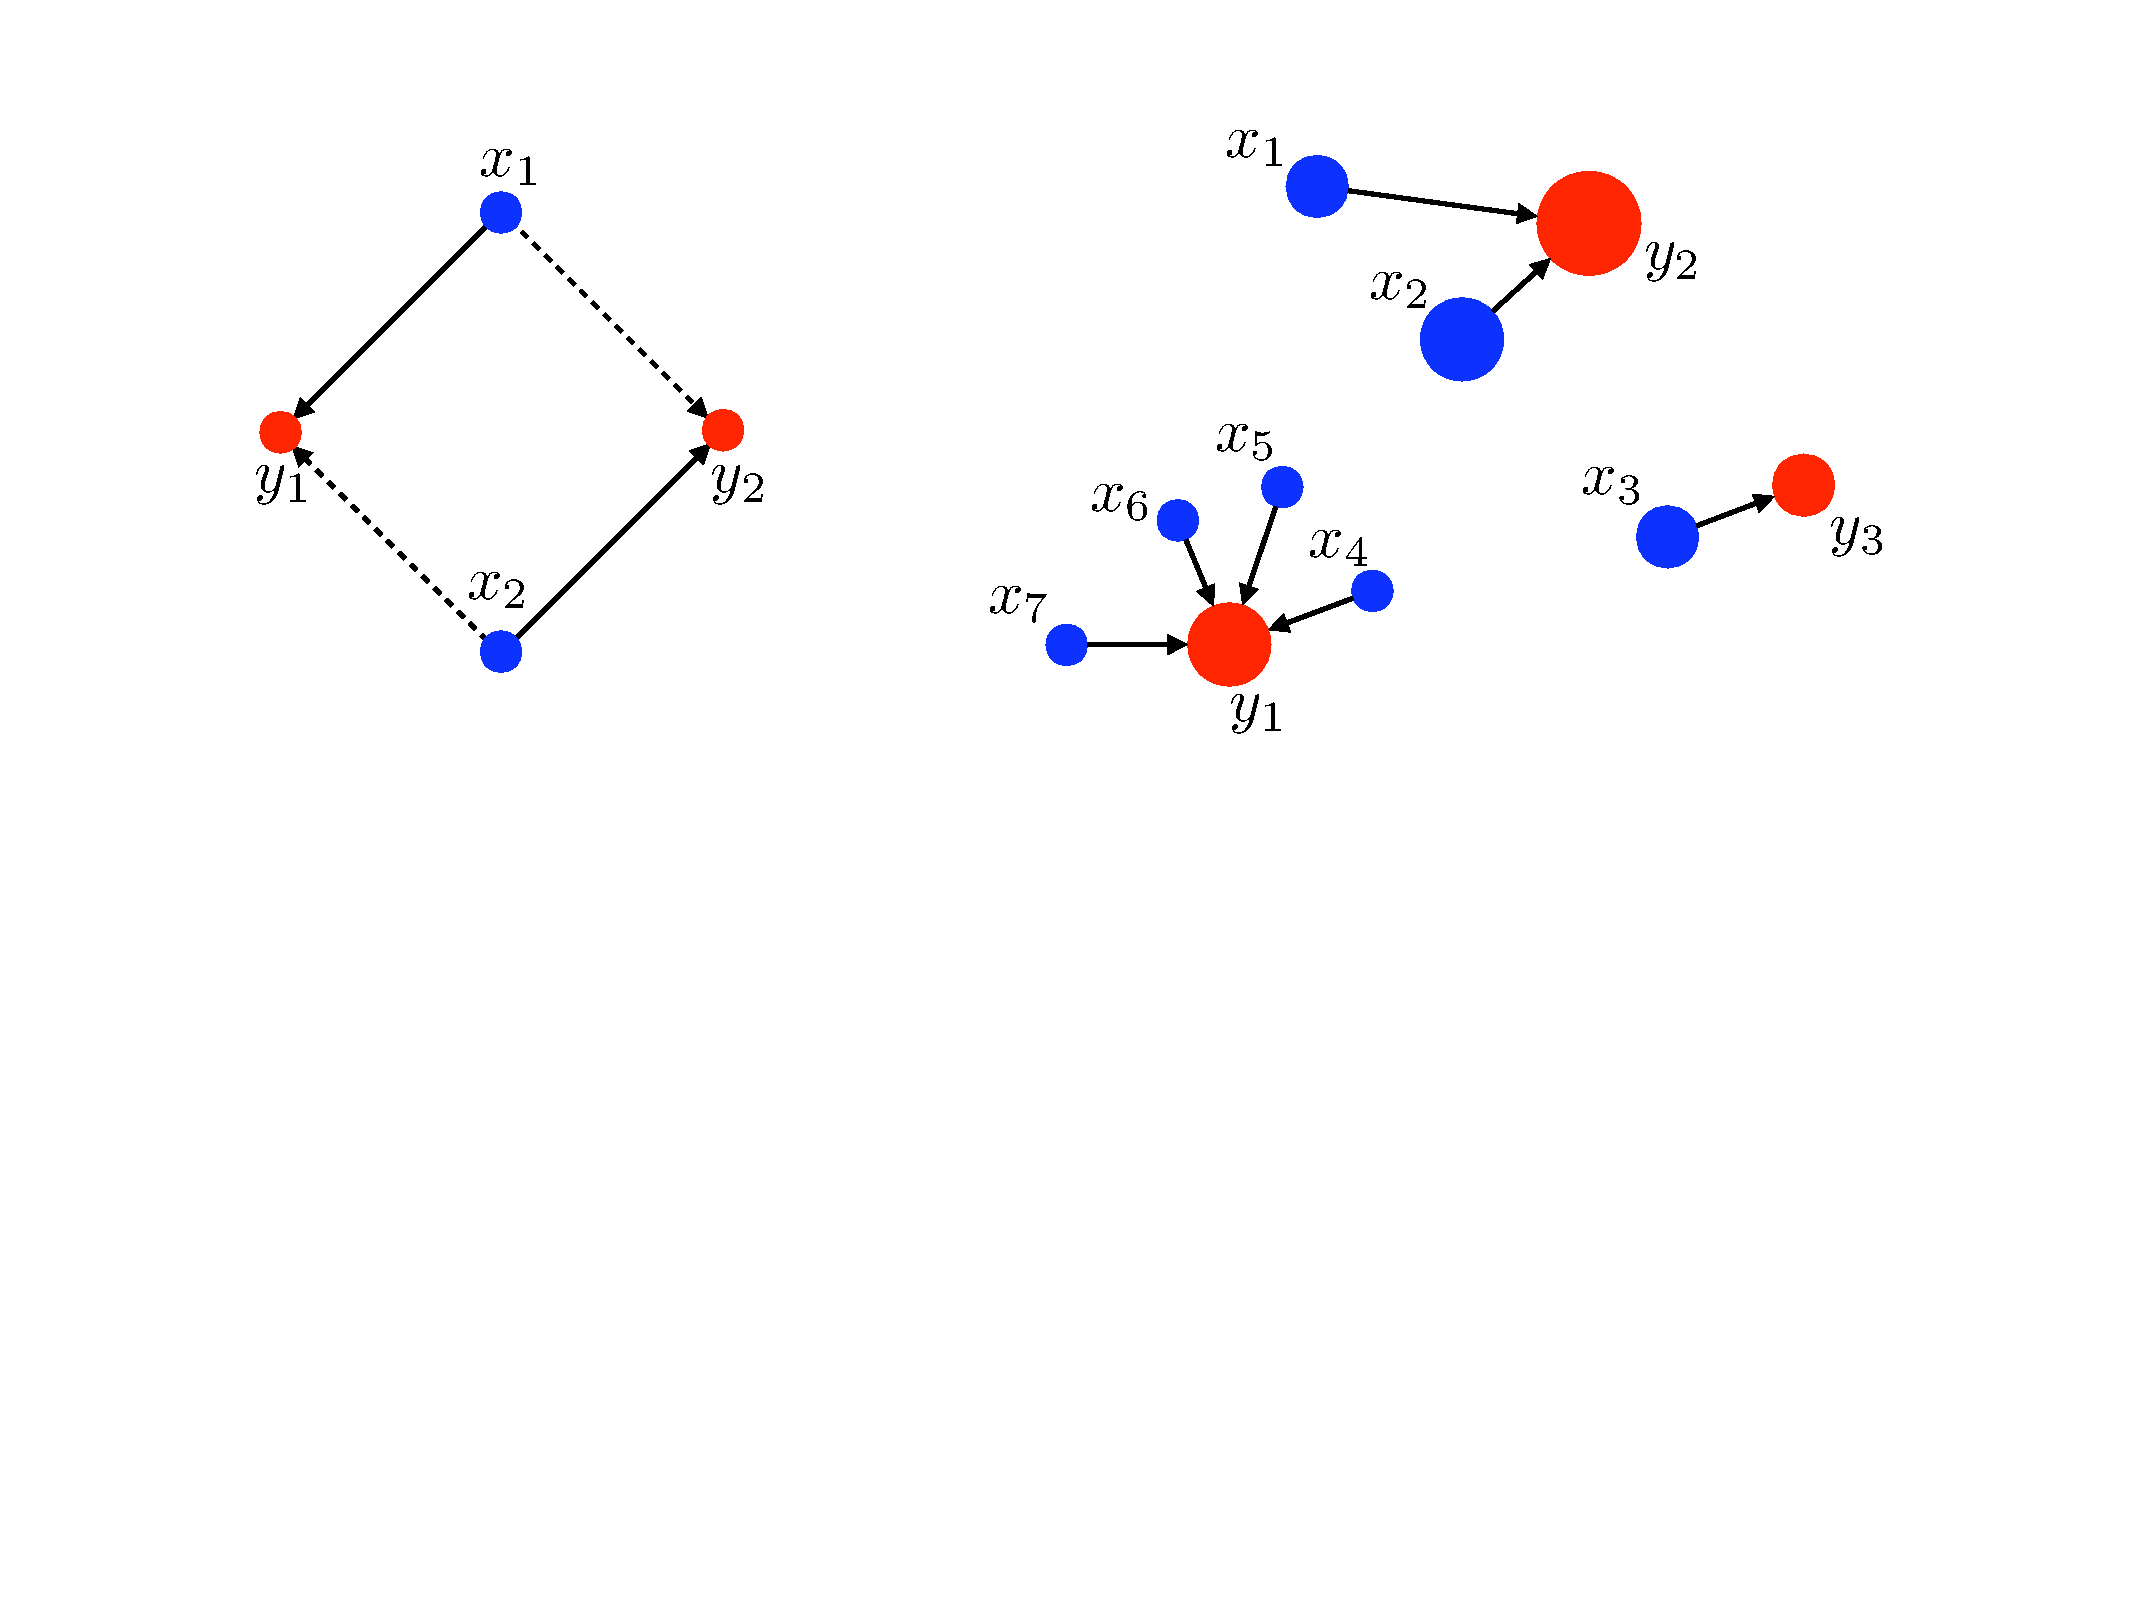
\includegraphics[width=.5\linewidth]{non-unique-optimal-matching/non-unique-optimal-matching}
\caption{\label{fig-non-unique-matching}
(left) blue dots from measure $\alpha$ and red dots from measure $\beta$ are pairwise equidistant. Hence, either matching $\sigma=(1,2)$ (full line) or $\sigma=(2,1)$ (dotted line) is optimal. (right) a Monge map can associate the blue measure $\alpha$ to the red measure $\beta$. The weights $\alpha_i$ are displayed proportionally to the area of the disk marked at each location. The mapping here is such that $T(x_1)=T(x_2)=y_2$, $T(x_3)=y_3$, whereas for $4\leq i\leq 7$ we have $T(x_i)=y_1$.
}
\end{figure}


\paragraph{1D case}

Here $\X=\RR$. Assuming $\al = \frac{1}{n}\sum_{i=1}^n \de_{x_i}$ and $\be = \frac{1}{n}\sum_{j=1}^n \de_{y_j}$, and assuming (without loss of generality) that the points are ordered, \emph{i.e.} $x_1 \leq x_2 \leq \ldots \leq x_n$ and $y_1 \leq y_2 \leq \ldots \leq y_n$, then one has the simple formula
\eql{\label{eq-1d-empirical}
	\Wass_p(\al,\be)^p = \sum_{i=1}^p |x_i-y_i|^p, 
}
\emph{i.e.} locally (if one assumes distinct points), $\Wass_p(\al,\be)$ is the $\ell^p$ norm between two vectors of ordered values of $\al$ and $\be$. That statement is only valid locally, in the sense that the order (and those vector representations) might change whenever some of the values change. That formula is a simple consequence of the more general remark given below. 
%
Figure~\ref{fig-1d-discrete}, top row, illustrates the 1-D transportation map between empirical measures with the same number of points. 
 The bottom row shows how this monotone map generalizes to arbitrary discrete measures. 
%
It is possible to leverage this 1-D computation to also compute efficiently OT on the circle, see~\cite{delon-circle}.  
%
Note that in the case of concave cost of the distance, for instance when $p<1$, the behaviour of the optimal transport plan is very different, see~\cite{delon-concave}, which describes an efficient solver in this case.



\begin{figure}
\centering
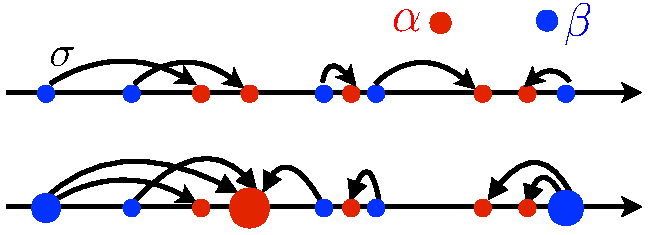
\includegraphics[width=.4\linewidth]{1d-discrete/1d-schematic}
\caption{\label{fig-1d-discrete}
1-D optimal couplings: each arrow $x_i \rightarrow y_j$ indicate a non-zero $\P_{i,j}$ in the optimal coupling.
% 
Top: empirical measures with same number of points (optimal matching).
Bottom: generic case. 
%
This corresponds to monotone rearrangements, if $x_i \leq x_{i'}$ are such that $\P_{i,j} \neq 0, \P_{i',j'} \neq 0$, then necessarily $y_j \leq y_{j'}$.
}
\end{figure}


- application to  Gray scale equalization, code via sorting , nlogn

%%%%%%%%%%%%%%%%%%%%%%%%%%%%%%%%%%%%%%%%%%%%%%%%%%%%%%%%%%%%%%%%%%%%%%%%%%%
\subsection{Matching Algorithms}

- Algorihtm : hungarian (explain intuitively) / auction (see later)
  Appli 3D color equalization
% !TEX root = ../CourseOT.tex

%%%%%%%%%%%%%%%%%%%%%%%%%%%%%%%%%%%%%%%%%%%%%%%%%%%%%%%%%%%%%%%%%%%%%%%%%%%
%%%%%%%%%%%%%%%%%%%%%%%%%%%%%%%%%%%%%%%%%%%%%%%%%%%%%%%%%%%%%%%%%%%%%%%%%%%
%%%%%%%%%%%%%%%%%%%%%%%%%%%%%%%%%%%%%%%%%%%%%%%%%%%%%%%%%%%%%%%%%%%%%%%%%%%
\section{Monge Problem between Measures}

%%%%%%%%%%%%%%%%%%%%%%%%%%%%%%%%%%%%%%%%%%%%%%%%%%%%%%%%%%%%%%%%%%%%%%%%%%%
\subsection{Measures}


%%%
\paragraph{Histograms}

We will interchangeably the term histogram or probability vector for any element $\a \in \simplex_n$ that belongs to the probability simplex
\eq{
	\simplex_n \eqdef \enscond{\a \in \RR_+^n}{ \sum_{i=1}^n \a_i = 1 }.
}


%%%
\paragraph{Discrete measure, empirical measure}

A discrete measure with weights $\a$ and locations $x_1,\dots,x_n\in\X$ reads
\eql{\label{eq-discr-meas}
	\al = \sum_{i=1}^n \a_i \de_{x_i}
}
where $\de_x$ is the Dirac at position $x$, intuitively a unit of mass which is infinitely concentrated at location $x$. Such as measure describes a probability measure if, additionally, $\a\in\simplex_n$, and more generally a positive measure if each of the ``weights'' described in vector $\a$ is positive itself. 
%
An ``empirical'' probability distribution is uniform on a point cloud, i.e. $\a=\frac{1}{n}\sum_i \de_{x_i}$. 
%
In practice, it many application is useful to be able to manipulate both the positions $x_i$ (``Lagrangian'' discretization) and the weights $\a_i$ (``Eulerian'' discretization). Lagrangian modification is usually more powerful (because it leads to adaptive discretization) but it breaks the convexity of most problems. 


%%%%
\paragraph{General measures}

We consider Borel measures $\al \in \Mm(\X)$ on a metric space $(\Xx,d)$, i.e. one can compute $\al(A)$ for any Borel set $A$ (which can be obtained by applying countable union, countable intersection, and relative complement to open sets). The measure should be finite, i.e. have a finite value on compact set.
%
A Dirac measure $\de_x$ is then define as $\de_x(A)=1$ is $x \in A$ and $0$ otherwise, and this extend by linearity for discrete measures of the form~\eqref{eq-discr-meas} as
\eq{
	\al(A) = \sum_{x_i \in A} \a_i  
}
%
We denote $\Mm_+(\X)$ the subset of all positive measures on $\X$, i.e. $\al(A) \geq 0$ (and $\al(\X)<+\infty$ for the measure to be finite). The set of probability measures is denoted $\Mm_+^1(\X)$, which means that any $\al \in \Mm_+^1(\X)$ is positive, and that $\al(\X)=1$. 


%%%%
\paragraph{Radon measures}

Using Lebesgue integration, a Borel measure can be used to compute integral of measurable functions (i.e. such that level sets $\enscond{x}{f(x) < t}$ are Borel sets), and we denote this pairing as
\eq{
	\dotp{f}{\al} \eqdef \int f(x) \d\al(x).
}
Integration of such a measurable $f$ against a discrete measure $\al$ computes a sum
\eq{ 
	\int_\X f(x) \d\al(x) = \sum_{i=1}^n \a_i f(x_i).
}

 
This can be in particular applied to the subspace of continuous functions which are measurable.
%
Integration against a finite measure on a compact space thus defines a continuous linear form $f \mapsto \int f \d\al$ on the Banach space of continuous functions $(\Cc(\Xx),\norm{\cdot}_\infty)$, indeed $|\int f \d\al| \leq \norm{f}_\infty |\al(\X)|$. 
%
On compact spaces, the converse is true, namely that any continuous linear form $\ell : f \mapsto \ell(f)$ on $(\Cc(\Xx),\norm{\cdot}_\infty)$ is represented as an integral against a measure $\ell(f)=\int f \d \al$. This is the  Riesz-Markov-Kakutani representation theorem, which is often stated that Borel measures can be identified to Radon measures.
%
Radon measures are thus in some sense ``less regular'' than functions, but more regular than distributions (which are dual to smooth functions). For instance, the derivative of a Dirac is not a measure.
%
This duality pairing $\dotp{f}{\al}$ between continuous function and measures will be crucial to develop duality theory for the convex optimization problem we will consider later. 

The associated norm, which is the norm of the linear form $\ell$, is the so-called total variation norm
\eq{
	\norm{\al}_{TV} = \norm{\ell}_{\Cc(\Xx)\rightarrow \RR} = \usup{f \in \Cc(\X)} \enscond{\dotp{f}{\al}}{ \norm{f}_\infty \leq 1 }.
}
(note that one can remove the $|\cdot|$ in the right hand side, and such a quantity is often called a ``dual norm'').
%
One can in fact show that this TV norm is the total mass of the absolute value measure $|\al|$.
%
The space $(\Mm(\Xx),\norm{\cdot}_{TV})$ is a Banach space, which is the dual of $(\Cc(\Xx),\norm{\cdot}_\infty)$. 

Recall that the absolute value of a measure is defined as 
\eq{
	|\al|(A) = \usup{A=\cup_i B_i} \sum_i |\al(B_i)|
}
so that for instance if $\al=\sum_i \a_i \de_{x_i}$, $|\al|=\sum_i |\a_i| \de_{x_i}$ and if $\d\al(x) = \rho \d x$ for a positif reference measure $\d x$, then $\d|\al|(x) = |\rho(x)| \d x$. 



%%%%%
\paragraph{Relative densities}

%TODO : ref measures
A measure $\al$ which is a weighting of another reference one $\d x$ is said to have a density, which is denoted $\d\al(x)=\density{\al}(x)\d x$  (on $\RR^d$ $\d x$ is often the Lebesgue measure), often also denoted $\density{\al} = \frac{\d\al}{\d x}$, which means that 
\eq{
	\foralls h \in \Cc(\RR^\dims), \quad
	\int_{\RR^\dims} h(x) \d\al(x) =  \int_{\RR^\dims} h(x) \density{\al}(x) \d x.
}

%%%%%
\paragraph{Probabilistic interpretation}

Radon probability measures can also be viewed as representing the distributions of random variables. A random variable $X$ on $\X$ is actually a map $X : \Om \rightarrow \X$ from some abstract (often un-specified) probabized space $(\Om,\PP)$, and its distribution is the Radon measure $\al \in \Mm_+^1(\X)$ such that $\PP(X \in A) = \al(A)=\int_A \d\al(x)$.


%%%%%%%%%%%%%%%%%%%%%%%%%%%%%%%%%%%%%%%%%%%%%%%%%%%%%%%%%%%%%%%%%%%%%%%%%%%
\subsection{Push Forward}
  
  
For some continuous map $\T : \X \rightarrow \Y$, we define the pushforward operator $\T_\sharp : \Mm(\X) \rightarrow \Mm(\Y)$. 
%
For a Dirac mass, one has $\T_\sharp \de_{x} = \de_{\T(x)}$, and this formula is extended to arbitrary measure by linearity. In some sense, moving from $\T$ to $\T_\sharp$ is a way to linearize any map at the prize of moving from a (possibly) finite dimensional space $\Xx$ to the infinite dimensional space $\Mm(\Xx)$, and this idea is central to many convex relaxation method, most notably Lasserre's relaxation.
%
For discrete measures~\eqref{eq-discr-meas}, the pushforward operation consists simply in moving the positions of all the points in the support of the measure
\eq{
	\T_{\sharp} \al \eqdef \sum_i \a_i \de_{\T(x_i)}.
}
For more general measures, for instance for those with a density, the notion of push-forward plays a fundamental to describe spatial modifications of probability measures. The formal definition reads as follow.

\begin{defn}[Push-forward]\label{defn-pushfwd}
For $\T : \X \rightarrow \Y$, the push forward measure $\be = \T_\sharp \al \in \Mm(\Y)$ of some $\al \in \Mm(\X)$ satisfies
\eql{\label{eq-push-fwd}
	\foralls h \in \Cc(\Y), \quad \int_\Y h(y) \d \be(y) = \int_\X h(\T(x)) \d\al(x).
	% = \int_X h(T(x)) \density{\al}(x) \d x %%%% y=T(x)   dy=|T'(x)| dx
	% = \int_Y h(y) \density{\al}(T^{-1}(y)) 1/|T'(x)| \d y 
	% = \int_Y h(y) \density{\be}(y) \d y
	%  \density{\al}(T^{-1}(y)) 1/|T'(x)| = \density{\be}(y)
}
Equivalently, for any measurable set $B \subset \Y$, one has
\eql{\label{eq-equiv-pushfwd}
	\be(B) = \al( \enscond{x \in \X}{\T(x) \in B} ).
}
Note that $\T_\sharp$ preserves positivity and total mass, so that if $\al \in \Mm_+^1(\X)$ then $\T_\sharp \al \in \Mm_+^1(\Y)$. 
\end{defn}

% Intuitively, a measurable map $T: \X\rightarrow \Y$, can be interpreted as a function ``moving'' a single point from a measurable space to another. The more general extension $T_\sharp$ can now ``move'' an entire probability measure on $\X$ towards a new probability measure on $\Y$. The operator $T_\sharp$ ``pushes forward'' each elementary mass of a measure $\al$ on $\X$ by applying the map $T$ to obtain then an elementary mass in $\Y$, to build on aggregate a new measure on $\Y)$ written $T_{\sharp}\al$.  Note that such a push-forward $\T_\sharp : \Mm_+^1(\X) \rightarrow \Mm_+^1(\Y)$ is a linear operator between measures in the sense that for two measures $\al_1,\al_2$ on $\X$, $T_\sharp(\al_1+\al_2)=T_\sharp\al_1+ T_\sharp\al_2$.



%%%%%%%
\begin{rem}[Push-forward for densities]
Explicitly doing the change of variable $x=T(x)$, so that $\d x = |\det(T'(x))| \d y$ in formula~\eqref{eq-push-fwd} for measures with densities $(\density{\al},\density{\be})$ on $\RR^\dims$ (assuming $\T$ is smooth and a bijection), one has for all $h \in \Cc(\Yy)$
\begin{align*}
	\int_\Yy h(y)\rho_\be(y) \d y &= \int_\Yy h(y) \d \be(y) = \int_\Xx h(T(x)) \d \al(x) = \int_\Xx h(T(x)) \rho_\al(x) \d x \\
		&= \int_\Yy h(y) \rho_\al(T^{-1}y) \frac{\d y}{|\det(T'( T^{-1} y))|}, 
\end{align*}
which shows that 
\eq{
	\rho_\be(y) = \rho_\al(T^{-1}y) \frac{1}{|\det(T'( T^{-1} y))|}.
}
Since $T$ is a diffeomorphism, one obtains equivalently
\eql{\label{eq-pfwd-density}
	\density{\al}(x) = |\det(\T'(x))|  \density{\be}(\T(x))
}
where $\T'(x) \in \RR^{\dims \times \dims}$ is the Jacobian matrix of $T$ (the matrix formed by taking the gradient of each coordinate of $T$).
%
This implies, denoting $y=\T(x)$
\eq{
	|\det(\T'(x))| = \frac{ \density{\al}(x) }{ \density{\be}(y) }.
}
\end{rem}
%%%%%%%


%%%%%%%%
%\begin{rem}[Push-forward vs. pull-back]
%The push-forward $\T_\sharp$ of measures should not be confounded with the pull-back of function $\T^\sharp : \Cc(\Y) \rightarrow \Cc(\X)$ which corresponds to the ``warping'' of functions. It is the linear map defined, for $g \in \Cc(\Y)$ by $\T^\sharp g = g \circ \T$. Push-forward and pull-back are actually adjoint one from each others, in the sense that
%\eq{
%	\foralls (\al,g) \in \Mm(\X) \times \Cc(Y), \quad
%	\int_\Y g \d( \T_\sharp\al ) = \int_\X (\T^\sharp g) \d\al.
%}
%It is important to realize that even if $(\al,\be)$ have densities $(\density{\al},\density{\be})$, $\T_\sharp \al$ is not equal to $\T^\sharp \density{\be}$, because of the presence of the Jacobian in~\eqref{eq-pfwd-density}.
%%
%This explains why OT should be used with caution to perform image registration, because it does not operate as an image warping method.
%%
%Figure~\ref{fig-push-pull} illustrate the distinction between these push-forward and pull-back operators. 
%\end{rem}
%%%%%%%%


%\begin{figure}
%\centering
%\begin{tabular}{@{}c@{\hspace{5mm}}c@{}}
%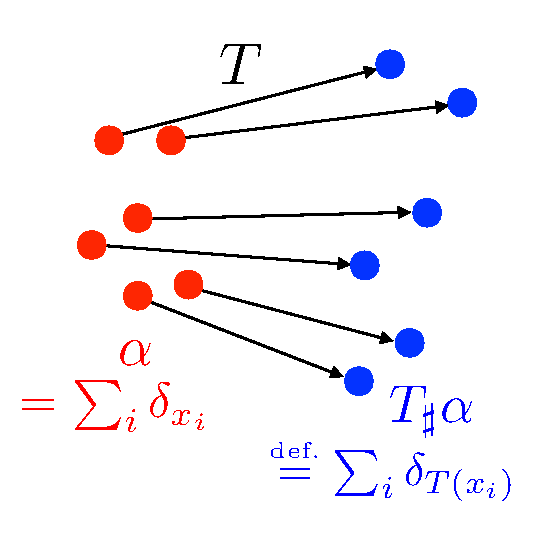
\includegraphics[width=.3\linewidth]{push-pull/push-forward}&
%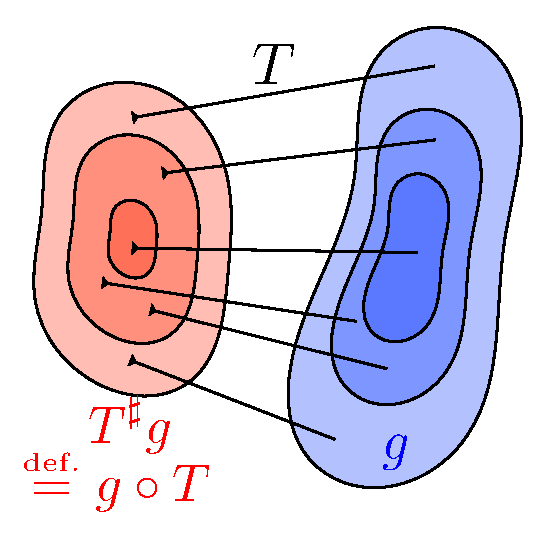
\includegraphics[width=.3\linewidth]{push-pull/pull-back}\\
%Push-forward of measures & Pull-back of functions
%\end{tabular}
%\caption{\label{fig-push-pull}
%Comparison of push-forward $\T_\sharp$ and pull-back $\T^\sharp$.
%}
%\end{figure}



\begin{rem}[Probabilistic interpretation]
A random variable $X$, equivalently, is the push-forward of $\PP$ by $X$, $\al=X_\sharp\PP$.
%
Applying another push-forward $\be = \T_\sharp\al$ for $\T : \X \rightarrow \Y$, following~\eqref{eq-push-fwd}, is equivalent to defining another random variable $Y=\T(X) : \om \in \Om \rightarrow \T(X(\om)) \in Y$, so that $\be$ is the distribution of $Y$.
%
Drawing a random sample $y$ from $Y$ is thus simply achieved by computing $y=\T(x)$ where $x$ is drawn from $X$. 
\end{rem}


%%%%%%%%%%%%%%%%%%%%%%%%%%%%%%%%%%%%%%%%%%%%%%%%%%%%%%%%%%%%%%%%%%%%%%%%%%%
\subsection{Monge's Formulation}


%%%%
\paragraph{Monge problem.}

Monge problem~\eqref{eq-optimal-assignment} is extended to the setting of two arbitrary probability measures $(\al,\be)$ on two spaces $(\X,\Y)$ as finding a map $\T : \X \rightarrow \Y$ that minimizes
\eql{\label{eq-monge-continuous}
	\uinf{\T} \enscond{ \int_{\X} \c(x,\T(x)) \d \al(x)  }{  \T_\sharp \al = \be }.
}
The constraint $\T_\sharp \al = \be$ means that $\T$ pushes forward the mass of $\al$ to $\be$, and makes use of the push-forward operator~\eqref{eq-push-fwd}. 

For empirical measure with same number $n=m$ of points, one retrieves the optimal matching problem. Indeed, this corresponds to the setting of empirical measures $\al=\sum_i \de_{x_i}$ and $\be=\sum_i \de_{y_i}$.  In this case, $\T_\sharp \al=\be$ necessarily implies that $\si$ is one-to-one, $\T : x_i \mapsto x_{\si(i)}$, so that 
\eq{
	\int_{\X} \c(x,\T(x)) \d \al(x) = \sum_i c(x_i,x_{\si(i)}).
}

In general, an optimal map $T$ solving~\eqref{eq-monge-continuous} might fail to exist. In fact, the constraint set $\T_\sharp \al = \be$, which is the case for instance if $\al=\de_x$ and $\be$ is not a single Dirac. 
%
Even if the constraint set is not empty the infimum might not be reached, the most celebrated example being the case of $\al$ being distributed uniformly on a single segment and $\be$ being distributed on two segments on the two sides.


%%%%
\paragraph{Monge distance.}

In the special case $c(x,y)=d^p(x,y)$ where $d$ is a distance, we denote 
\eql{\label{eq-monge-distance}
	\tilde\Wass_p^p(\al,\be) \eqdef 
		\uinf{\T} \enscond{ \Ee_\al(T) \eqdef \int_{\X} d(x,\T(x))^p \d \al(x)  }{  \T_\sharp \al = \be }.
}
If the constraint set is empty, then we set $\tilde \Wass_p^p(\al,\be) = +\infty$.
%
The following proposition shows that quantity defines a distance.

\begin{prop}
	$\tilde \Wass$ is a distance.
\end{prop}
\begin{proof}
	If $\tilde \Wass_p^p(\al,\be)=0$ then necessarily the optimal map is $\Id$ on the support of $\al$ and $\be=\al$.
	%
	Let us prove that $\tilde \Wass_p^p(\al,\be) \leq \tilde \Wass_p^p(\al,\ga)+\tilde \Wass_p^p(\ga,\be)$.
	If $\tilde \Wass_p^p(\al,\be)=+\infty$, then either $\tilde \Wass_p^p(\al,\ga)=+\infty$ or $\tilde \Wass_p^p(\ga,\be)=+\infty$, because otherwise we consider two maps $(S,T)$ such that $S_\sharp \al=\ga$ and $T_\sharp \ga=\be$ and then $(T \circ S)_\sharp \al = \be$ so that 
	$\tilde \Wass_p^p(\al,\be) \leq \Ee_\al(S \circ T) < +\infty$.
	%
	So necessarily $\tilde \Wass_p^p(\al,\be)<+\infty$ and we can restrict our attention to the cases 
	where $\tilde \Wass_p^p(\al,\ga)<+\infty$ and $\tilde \Wass_p^p(\ga,\be)<+\infty$ because otherwise the inequality is trivial.
	%
	For any $\epsilon>0$, we consider $\epsilon$-minimizer $S_\sharp \al=\ga$ and $T_\sharp \ga=\be$ such that
	\eq{
		E_\al(S)^{\frac{1}{p}} \leq \tilde \Wass_p(\al,\ga)+\epsilon
		\qandq
		E_\ga(T)^{\frac{1}{p}} \leq \tilde \Wass_p(\ga,\be)+\epsilon.
	}
	%
	Now we have that $(T \circ S)_\sharp \al=\ga$, so that 
	one has, using sub-optimality of this map and the triangular inequality 
	\eq{
		\Wass_p(\al,\ga) \leq \int d(x,T(S(x)))^p \d\al(x)^{\frac{1}{p}}
			\leq
			\int (d(x,S(x)) + d(S(x),T(S(x))))^p \d\al(x)^{\frac{1}{p}}	.		
	}
	The using Minkowski inequality
	\eq{
		\Wass_p(\al,\ga) \leq
			\int d(x,S(x))^p \d\al(x)^{\frac{1}{p}}	
			+ 		
			\int d(S(x),T(S(x)))^p \d\al(x)^{\frac{1}{p}}	
		\leq \Wass_p(\al,\be) + \Wass_p(\be,\ga) + 2 \epsilon.
	}
	Letting $\epsilon \rightarrow 0$ gives the result. 
\end{proof}

%%%%%%%%%%%%%%%%%%%%%%%%%%%%%%%%%%%%%%%%%%%%%%%%%%%%%%%%%%%%%%%%%%%%%%%%%%%
\subsection{Existence and Uniqueness of the Monge Map}

%%%%
\paragraph{Brenier's theorem.}

The following celebrated theorem of~\cite{Brenier91} ensures that in $\RR^\dims$ for $p=2$, if at least one of the two inputs measures has a density, then Kantorovitch and Monge problems are equivalent.

\begin{thm}[Brenier]\label{thm-brenier}
	In the case $\X=\Y=\RR^\dims$ and $c(x,y)=\norm{x-y}^2$, if $\al$ has a density with respect to the Lebesgue measure, then there exists a unique optimal Monge map $\T$. This map is characterized by being the unique gradient of a convex function $\T=\nabla \phi$ such that $(\nabla \phi)_\sharp \al = \be$. 
\end{thm}

Its proof requires to study the relaxed Kantorovitch problems and its dual, so we defer it to later (Section~\ref{sec-c-transfo}). 


%This results shows that in the setting of $\Wass_2$ with non-singular densities, the Monge problem~\eqref{eq-monge-continuous} and its Kantorovich relaxation~\eqref{eq-mk-generic} are equal (the relaxation is tight). This is the continuous analog of Proposition~\ref{prop-matching-kanto} for the assignment case~\eqref{prop-matching-kanto}, which states that the minimum of the optimal transport problem is achieved, when the marginals are equal and uniform, at a permutation matrix (a discrete map).
%
Brenier's theorem, stating that an optimal transport map must be the gradient of a convex function, should be examined under the light that a convex function is a natural generalization of the notion of increasing functions in dimension more than one. 
%
For instance, the gradient of a convex function is a monotone gradient field in the sense
\eq{
	\foralls (x,x') \in \RR^d \times \RR^d, \quad 
	\dotp{\nabla\phi(x)-\nabla\phi(x')}{x-x'} \geq 0.
}
Note however that in dimension larger than 1, not all monotone fields are gradient of convex function. For instance, a rotation is monotone but can never be an optimal transport because a gradient field $Ax$ defined by a linear map $A$ is necessarily obtained by a symmetric matrix $A$. Indeed, such a linear field must be associated to a quadratic form $\phi(x)=\dotp{Bx}{x}/2$
and hence $A=\nabla \phi = (B+B^\top)/2$.
%
Optimal transport can thus plays an important role to define quantile functions in arbitrary dimensions, which in turn is useful for applications to quantile regression problems~\cite{carlier2016vector}.
 

Note also that this theorem can be extended in many directions.  
% 
The condition that $\al$ has a density can be weakened to the condition that it does not give mass to ``small sets'' having Hausdorff dimension smaller than $\dims-1$ (e.g. hypersurfaces). 
%
One can also consider costs of the form $\c(x,y)=h(x-y)$ where $h$ is a strictly convex smooth function, for for instance $c(x,y)=\norm{x-y}^p$ with $1<p<+\infty$. 

Note that Brenier's theorem provides existence and uniqueness, but in general, the map $\T$ can be very irregular. 
%
Indeed, $\phi$ is in general non-smooth, but it is in fact convex and Lipschitz, so that $\nabla \phi$ is actually well defined $\al$-almost everywhere. Ensuring $\T$ to be smooth actually requires the target $\be$ to be regular, and  more precisely its support must be convex.

If $\al$ does not have a density, then $\T$ might fail to exists and it should be replaced by a set-valued function included in $\partial\phi$ which is now the sub-differential of a convex function, which might have singularity on a non-zero measure set. This means that $\T$ can ``split'' the mass by mapping to several locations  $T(x) \subset \partial\phi$. Actually, the condition that $T(x) \subset \partial\phi(x)$ and $\T_\sharp \al=\be$ implies that the multi-map $\T$ defines a solution of Kantorovitch problem that will be studied later. 



%%%%%%%
\paragraph{Monge-Amp\`ere equation.}

For measures with densities, using~\eqref{eq-pfwd-density}, one obtains that $\phi$ is the unique (up to the addition of a constant) convex function which solves the following Monge-Ampère-type equation
\eql{\label{eq-monge-ampere}
	\det(\partial^2\phi(x))  \density{\be}(\nabla\phi(x)) = \density{\al}(x)
}
where $\partial^2\phi(x) \in \RR^{\dims \times \dims}$ is the hessian of $\phi$. 
%
The convexity constraint forces $\det(\partial^2\phi(x)) \geq 0$ and is necessary for this equation to have a solution and be well-posed. 
%
The Monge-Amp\`ere operator $\det(\partial^2\phi(x))$ can be understood as a non-linear degenerate Laplacian. In the limit of small displacements, one can consider $\phi(x)=\norm{x}^2/2 + \epsilon\psi$ so that $\nabla \phi = \Id+\epsilon \nabla \psi$, one indeed recovers the Laplacian $\Delta$ as a linearization since for smooth maps
\eq{
	\det(\partial^2\phi(x)) = 1 + \epsilon \Delta \psi(x) + o(\epsilon), 
}
where we used the fact that $\det(\Id+\epsilon A) = 1+\epsilon\tr(A)+o(\epsilon)$. 



%%%%%%%
\paragraph{OT in 1-D.}

For a measure $\al$ on $\RR$, we introduce the cumulative function
\eql{\label{eq-cumul-defn}
	\foralls x \in \RR, \quad \cumul{\al}(x) \eqdef \int_{-\infty}^x \d\al, 
}
which is a function $\cumul{\al} : \RR \rightarrow [0,1]$.
%
Its pseudo-inverse  $\cumul{\al}^{-1} : [0,1] \rightarrow \RR \cup \{-\infty\}$ 
\eq{
	\foralls r \in [0,1], \quad \cumul{\al}^{-1}(r) = \umin{x} \enscond{x \in \RR \cup \{-\infty\} }{ \cumul{\al}(x) \geq r }.
}
That function is also called the quantile function of $\alpha$. 
%
The following proposition shows that these defines push-forward toward the uniform distribution $\Uu$ on $[0,1]$.

\begin{prop}
	One has $(\Cc_\al)^{-1}_\sharp \Uu = \al$,  
	where $\Uu$ is the uniform distribution in $[0,1]$. 
	%
	If $\al$ has a density, then $(\Cc_\al)_\sharp \al = \Uu$.
\end{prop}
\begin{proof}
	For simplicity, we assume $\al$ has a strictly positive density, so that $\Cc_\al$ is a strictly increasing continuous function.
	%
	Denoting $\ga \eqdef (\Cc_\al)^{-1}_\sharp \Uu$ we aim at proving $\ga=\al$, which is equivalent to 
	$\Cc_\ga=\Cc_\al$. One has
	\eq{
		\Cc_\ga(x) = \int_{-\infty}^x \d \ga = \int_\RR 1_{]-\infty,x]} \d( (\Cc_\al^{-1})_\sharp \Uu)
		  	 = \int_0^1 1_{]-\infty,x]}(\Cc_\al^{-1}(z)) \d z
			 = \int_0^1 1_{[0,\Cc_\al(x)]}(z) \d z
			 = \Cc_\al(x)
	}
	where we use the fact that 
	\eq{
		-\infty \leq \Cc_\al^{-1}(z) \leq x 
		\quad\Longleftrightarrow
		0 \leq z \leq \Cc_\al(x).
	}
\end{proof}

%
If $\al$ has a density, this shows that the map
\eql{\label{eq-OT-map-1d}
 	\T = \cumul{\be}^{-1} \circ \cumul{\al}
}
satisfies $\T_\sharp \al = \be$. 

For the cost $c(x,y)=|x=y|^2$, since this $\T$ is increasing (hence the gradient of a convex function since we are in 1-D), by Brenier's theorem, $\T$ is the solution to Monge problem (at least if we impose that $\al$ has a density, otherwise it might lead to a solution of Kantorovitch problem by properly defining the pseudo-inverse). 
%
This closed form formula is also optimal for any cost of the form $h(|x-y|)$ for increasing $h$. 
%
For discrete measures, one cannot apply directly this reasoning (because $\al$ does not have a density), but if the measure are uniform on the same number of Dirac masses, then this approach is actually equivalent to the sorting formula. 

Plugging this optimal map into the definition of the ``Wasserstein'' distance (we will see later that this quantity defines a distance), so that for any $p \geq 1$, one has
\eql{\label{eq-wass-cumul}
	\Wass_p(\al,\be)^p =
	\int_\RR |x- \cumul{\be}^{-1}( \cumul{\al}(x) )| \d \al(x)
	= \int_0^1 | \cumul{\al}^{-1}(r) - \cumul{\be}^{-1}(r) |^p \d r = 	
	 \norm{ \cumul{\al}^{-1} - \cumul{\be}^{-1} }_{L^p([0,1])}^p .
}
This formula is still valid for any measure (one can for instance approximate $\al$ by a measure with density). 
%
This formula means that through the map $\al \mapsto \cumul{\al}^{-1}$, the Wasserstein distance is isometric to a linear space equipped with the $L^p$ norm. For $p=2$, the Wasserstein distance for measures on the real line is thus a Hilbertian metric. 
This makes the geometry of 1-D optimal transport very simple, but also very different from its geometry in higher dimensions, which is not Hilbertian.
% as discussed in Proposition~\ref{prop-negative-definite} and more generally in~\S\ref{sec-non-embeddability}.

For $p=1$, one even has the simpler formula. Indeed, the previous formula is nothing more than the area between the two graphs of the copula, which can thus be computed by exchanging the role of the two axis, so that 
\begin{align}\label{eq-w1-1d}
	\Wass_1(\al,\be) &= \norm{ \cumul{\al} - \cumul{\be} }_{L^1(\RR)} = 
	\int_\RR | \cumul{\al}(x) - \cumul{\be}(x) | \d x 
	= \int_\RR \abs{ \int_{-\infty}^x \d(\al-\be) } \d x.
\end{align}
which shows that $\Wass_1$ is a norm (see~\S\ref{sec-w1-eucl} for the generalization to arbitrary dimensions). 

It is possible to define other type of norm which behave similarly (i.e. metrize the convergence in law), for instance $\norm{ \cumul{\al} - \cumul{\be} }_{L^p(\RR)}$ define respectively the Wasserstein, Cramer (i.e. Sobolev) and Kolmogorov-Smirnov norms for $p=1,2,\infty$. 



% Figure~\ref{fig-1d-ot} illustrates the computation of 1-D OT through cumulative functions. It also displays displacement interpolations, computed as detailed in~\eqref{eq-displacement-1d-cumul}, see also Remark~\ref{rem-bary-1d}. For a detailed survey of the properties of optimal transport in 1-D, we refer the reader to~\cite[Chapter 2]{SantambrogioBook}.


%
%\newcommand{\MyFigCumulMeas}[1]{\includegraphics[width=.28\linewidth]{1d-cumulative/#1}}
%\newcommand{\MyFigCumulCum}[1]{\includegraphics[width=.2\linewidth]{1d-cumulative/#1}}
%\begin{figure}
%\centering
%\begin{tabular}{@{}c@{\hspace{1mm}}c@{\hspace{1mm}}c@{}}
%\MyFigCumulMeas{input-mu}&
%\MyFigCumulMeas{input-nu}&
%\MyFigCumulMeas{interp-bary}\\
%$\mu$ & $\nu$ & ${ (t\T+(1-t)\Id)_\sharp \mu}$
%\end{tabular}
%%%%%
%\begin{tabular}{@{}c@{\hspace{2mm}}c@{\hspace{2mm}}c@{\hspace{2mm}}c@{}}
%\MyFigCumulCum{cumul}&
%\MyFigCumulCum{icumul}&
%\MyFigCumulCum{transports}&
%\MyFigCumulCum{interp-cumul}\\
%$(\cumul{\al},\cumul{\be})$ & 
%$(\cumul{\al}^{-1},\cumul{\be}^{-1})$ & 
%$(T,T^{-1})$ &
%$(1-t)\cumul{\al}^{-1}+t\cumul{\be}^{-1}$ 
%\end{tabular}
%\caption{\label{fig-1d-ot}
%Computation of OT and displacement interpolation between two 1-D measures, using cumulant function as detailed in~\eqref{eq-OT-map-1d}. 
%}
%\end{figure}




%%%%%%%
\paragraph{OT on 1-D Gaussians}

We first consider the case where $\al = \Nn(m_\al,s_\al^2)$ and $\be = \Nn(m_\be,s_\be^2)$ are two Gaussians in $\RR$. 
%
Then one verifies that 
\eq{
	\T(x) = \frac{s_\be}{s_\al}(x-m_\al)+m_\be
}
satisfies $\T_\sharp \al=\be$, furthermore it is the the derivative of the convex function 
\eq{
	\phi(x) = \frac{s_\be}{2s_\al}(x-m_\al)^2+m_\be x, 
}
so that according to Brenier's theorem, for the cost $c(x-y)=(x-y)^2$, $\T$ is the unique optimal transport, and the associated Monge distance is, after some computation
\eq{
	\tilde\Wass_2^2(\al,\be) = \int_\RR \pa{\frac{s_\be}{s_\al}(x-m_\al)+m_\be - x}^2 \d \al(x) = 
	(m_\al-m_\be)^2 + (s_\al-s_\be)^2.
}
This formula still holds for Dirac masses, i.e. if $s_\al=0$ or $s_\be=0$.
%
The OT geometry of Gaussians is thus the Euclidean distance on the half plane $(m,s) \in \RR \times \RR_+$.
%
This should be contrasted with the geometry of $\KL$, where singular Gaussians (for which $s=0$) are infinitely distant. 

%%%%%%%
\paragraph{OT on Gaussians}


If $\al = \Nn(\mean_\al,\cov_\al)$ and $\be = \Nn(\mean_\be,\cov_\be)$ are two Gaussians in $\RR^\dims$, we now look for an affine map
\eql{\label{eq-transport-Bures}
	\T: x \mapsto \mean_\be + A(x-\mean_\al).
}
This map is the gradient of the convex function $\phi(x) = \dotp{\mean_\be}{x} + \dotp{A(x-\mean_\al)}{x-\mean_\al}/2$ if and only if $A$ is a symmetric positive matrix. 

\begin{prop}
One has $\T_\sharp \al=\be$ if and only if 
\eql{\label{eq-gauss-pf}
	A \cov_\al A = \cov_\be.
}
\end{prop}
\begin{proof}
Indeed, one simply has to notice that the change of variables formula~\eqref{eq-pfwd-density} is satisfied since
$$
\begin{aligned}\rho_\be(T(x))&=\det(2\pi\cov_\be)^{-\tfrac{1}{2}} \exp(-\dotp{T(x)-\mean_\be}{\cov_\be^{-1}(T(x)-\mean_\be)})\\
&= \det(2\pi\cov_\be)^{-\tfrac{1}{2}} \exp(-\dotp{ x-\mean_\al}{\transp{A}\cov_\be^{-1}A(x-\mean_\al)}) \\
&= \det(2\pi\cov_\be)^{-\tfrac{1}{2}} \exp(-\dotp{ x-\mean_\al}{\cov_\al^{-1}(x-\mean_\al)}),
\end{aligned}$$
and since $T$ is a linear map we have that 
$$|\det T'(x)|= \det A = \left(\frac{\det\cov_\be}{\det\cov_\al}\right)^{\tfrac{1}{2}}$$
 and we therefore recover $\rho_\al=|\det T'| \rho_\be$ meaning $T_\sharp \al = \be$. 
\end{proof}

Equation~\eqref{eq-gauss-pf} is a quadratic equation on $A$. Using the square root of positive matrices, which is uniquely defined, one has 
\eq{
	\cov_\al^{\frac{1}{2}} \cov_\be \cov_\al^{\frac{1}{2}}
	=
	 \cov_\al^{\frac{1}{2}} A \cov_\al A \cov_\al^{\frac{1}{2}} =  
	 (\cov_\al^{\frac{1}{2}} A \cov_\al^{\frac{1}{2}})^2, 
}
so that this equation has a unique solution, given by
\eq{
	A=\cov_\al^{-\tfrac{1}{2}}\Big(\cov_\al^{\tfrac{1}{2}}\cov_\be\cov_\al^{\tfrac{1}{2}}\Big)^{\tfrac{1}{2}}\cov_\al^{-\tfrac{1}{2}}=\transp{A}.
}
Using Brenier's theorem~\cite{Brenier91}, we conclude that $\T$ is optimal. 
 
With additional calculations involving first and second order moments of $\rho_\al$, we obtain that the transport cost of that map is
\eql{\label{eq-dist-gauss}
	\tilde\Wass_2^2( \al,\be ) = \norm{ \mean_\al - \mean_\be }^2 + \Bb(\cov_\al,\cov_\be)^2
}
where $\Bb$ is the so-called Bures' metric~\cite{bures1969extension} between positive definite matrices (see also~\cite{,forrester2016relating}),
\eql{\label{eq-bure-defn}
	\Bb(\cov_\al,\cov_\be)^2 \eqdef \tr\pa{
		\cov_\al + \cov_\be - 2 ( \cov_\al^{1/2} \cov_\be \cov_\al^{1/2} )^{1/2}
	},
}
where $\cov^{1/2}$ is the matrix square root. One can show that $\Bb$ is a distance on covariance matrices, and that $\Bb^2$ is convex with respect to both its arguments. 
%
In the case where $\cov_\al = \diag(r_i)_i$ and $\cov_\be = \diag(s_i)_i$ are diagonals, the Bures metric is the Hellinger distance
\eq{
	\Bb(\cov_\al,\cov_\be) = \norm{ \sqrt{r}-\sqrt{s} }_2.
}
%
% For a detailed treatment of the Wasserstein geometry of Gaussian distributions, we refer to~\cite{takatsu2011wasserstein}.


% !TEX root = ../CourseOT.tex

%%%%%%%%%%%%%%%%%%%%%%%%%%%%%%%%%%%%%%%%%%%%%%%%%%%%%%%%%%%%%%%%%%%%%%%%%%%
%%%%%%%%%%%%%%%%%%%%%%%%%%%%%%%%%%%%%%%%%%%%%%%%%%%%%%%%%%%%%%%%%%%%%%%%%%%
%%%%%%%%%%%%%%%%%%%%%%%%%%%%%%%%%%%%%%%%%%%%%%%%%%%%%%%%%%%%%%%%%%%%%%%%%%%
\section{Kantorovitch Relaxation}

%%%%%%%%%%%%%%%%%%%%%%%%%%%%%%%%%%%%%%%%%%%%%%%%%%%%%%%%%%%%%%%%%%%%%%%%%%%
\subsection{Discrete Relaxation}

Monge discrete matching problem is problematic because it cannot be applied when $n \neq m$. One needs to take into account masses $(\a_i,\b_j)$ to handle this more general situation. 
%
Monge continuous formulation~\eqref{eq-monge-continuous} using push-forward is also problematic because it can be the case that there is no transport map $T$ such that $T_\sharp \al = \be$, for instance when $\al$ is made of a single Dirac to be mapped to several Dirac. Associated to this, it is not symmetric with respect to exchange of $\al$ and $\be$ (one can map two Diracs to a single one, but not the other way).
%
Also, these are non-convex optimization problem which are not simple to solve numerically. 
 
The key idea of~\cite{Kantorovich42} is to relax the deterministic nature of transportation, namely the fact that a source point $x_i$ can only be assigned to another, or transported to one and one location $T(x_i)$ only. Kantorovich proposes instead that the mass at any point $x_i$ be potentially dispatched across several locations. Kantorovich moves away from the idea that mass transportation should be ``deterministic'' to consider instead a ``probabilistic'' (or ``fuzzy'') transportation, which allows what is commonly known now as ``mass splitting'' from a source towards several targets. This flexibility is encoded using, in place of a permutation $\sigma$ or a map $T$, a coupling matrix $\P  \in \RR_+^{n \times m}$, where $\P_{i,j}$ describes the amount of mass flowing from bin $i$ (or point $x_i$) towards bin $j$ (or point $x_j$), 
$x_i$ towards $y_j$ in the formalism of discrete measures $\al=\sum_i \a_i \de_{x_i}$, $\be=\sum_j \b_j \de_{y_j}$. Admissible couplings are only constrained to satisfy the conservation of mass
\eql{\label{eq-discr-couplings}
	\CouplingsD(\a,\b) \eqdef \enscond{ \P \in \RR_+^{n \times m} }{
		\P \ones_m = \a \qandq 
		\transp{\P} \ones_n = \b	
	},
}
where we used the following matrix-vector notation
\eq{
	\P \ones_m = \left(\sum_j \P_{i,j}\right)_i \in \RR^n
	\qandq
	\transp{\P} \ones_n = \left(\sum_i \P_{i,j}\right)_j \in \RR^m. 
}
The set of matrices $\CouplingsD(\a,\b)$ is bounded, defined by $n+m$ equality constraints, and therefore a convex polytope (the convex hull of a finite set of matrices).

%
Additionally, whereas the Monge formulatio is intrinsically asymmetric, Kantorovich's relaxed formulation is always symmetric, in the sense that a coupling $\P$ is in  $\CouplingsD(\a,\b)$ if and only if  $\transp{\P}$ is in $\CouplingsD(\b,\a)$.

Kantorovich's optimal transport problem now reads
\eql{\label{eq-kanto-discr} 
	\MKD_{\C}(\a,\b) \eqdef 
	\umin{\P \in \CouplingsD(\a,\b)}
		\dotp{\C}{\P} \eqdef \sum_{i,j} \C_{i,j} \P_{i,j}. 
}
This is a linear program, and as is usually the case with such programs, its solutions are not necessarily unique. 



%%%%%%%%%%
\paragraph{Linear programming algorithms.}

The reference algorithms to solve~\eqref{eq-mk-discr} are network simplexes. There exists instances of this method which scale like  $O(n^3 \log n)$. Alternative include interior points, which are usually inferior on this particular type of linear program.

%%%%%%%%%%
\paragraph{1-D cases.}

In 1-D, if $c(x,y)=|x-y|^p$ on $\Xx=\Yy=\RR$ with $p \geq 1$, then an optimal transport map is given by an increasing map. So as explained in~\eqref{sec-monge-pbm}, the case $n=m$ and $\a_i=\b_j=\frac{1}{n}$ is solved in $O(n \log(n))$ operations. 
%
In the general case, an optimal coupling matrix $\P$ can be computed similarly in $O(n\log(n)+m\log(m))$ by sorting the points and then sweeping the mass in a single pass from left to right \todo{explain more}.


%%%%%%%%%%
\paragraph{Permutation Matrices as Couplings} 

We restrict our attention to the special case $n=m$ and $\a_i=\b_i=1$ (up to a scaling by $1/n$, these are thus probability measures).
%
In this case one can solve Monge optimal matching problem~\eqref{eq-optimal-assignment}, and it is convenient to re-write it using permutation matrices. 
%
For a permutation $\si\in\Perm(n)$, we write $\P_{\si}$ for the corresponding permutation matrix,
\eql{\label{eq-perm-matrices}
		\foralls (i,j) \in \range{n}^2, \quad
		(\P_{\si})_{i,j} = \choice{
			1 \qifq j=\si_i, \\
			0 \quad\text{otherwise.} 
		}
} 
We denote the set of permutation matrices as
\eq{
	\Pp_n \eqdef \enscond{\P_\si}{ \si\in\Perm(n) }, 
}
which is a discrete, hence non-convex, set. One has
\eq{
	\dotp{\C}{\P_{\si}} = \sum_{i=1}^n \C_{i,\si_i}
}
so that~\eqref{eq-optimal-assignment} is equivalent to the non-convex optimization problem
\eq{
	\umin{\P \in \Pp_n} \dotp{\C}{\P}. 
}

In contrast, one has that $\CouplingsD(\a,\b) = \Bb_n$ is equal to the convex set of bistochastic matrices 
\eq{
	\Bb_n \eqdef \enscond{ \P \in \RR_+^{n \times n} }{\P \ones_n = \P^\top \ones_n = \ones_n}
}
so that Kantorovitch problem reads 
\eq{
	\umin{\P \in \Bb_n} \dotp{\C}{\P}. 
}
The set of permutation matrices is strictly included in the set of bistochastic matrices, and more precisely
\eq{
	\Pp_n = \Bb_n \cap \{0,1\}^{n \times n}.
}
This shows that one has the following obvious relation between the cost of Monge and Kantorovitch problem
\eq{
	\umin{\P \in \Bb_n} \dotp{\C}{\P} \leq \umin{\P \in \Pp_n} \dotp{\C}{\P}. 
}
We will now show that there is in fact an equality between these two costs, so that both problems are in some sense equivalent. 


For this, we will make a detour through more general linear optimization problem of the form $\umin{\P \in \Cc} \dotp{\C}{\P}$ for some compact convex set $\Cc$. We firs introduce the notion of extremal point, which are intuitively the vertices of $\Cc$
\eq{
	\text{Extr}(\Cc) \eqdef \enscond{\P}{ \foralls (Q,R) \in \Cc^2, \P = \frac{Q+R}{2} \Rightarrow Q=R }.
}
So to show that $\P \notin \text{Extr}(\Cc)$ is suffices to split $\P$ as $\P = \frac{Q+R}{2}$ with $Q \neq R$ and $(Q,R) \in \Cc^2$.
%
We will assume the following fundamental result.

\begin{prop}
	If $\Cc$ is compact, then $\text{\upshape Extr}(\Cc) \neq 0$.
\end{prop}

The fact that $\Cc$ is compact is crucial, for instance the set $\enscond{(x,y) \in \RR_+^2}{ xy \geq 1}$ has no extremal point. 

We can now use this result to show the following fundamental result, namely that there is always a solution to a linear program which is an extremal point.
% 
Note that of course the set of solution (which is non-empty because one minimizes a continuous function on a compact) might not be a singleton. 


\begin{figure}
\centering
\begin{tabular}{@{}c@{\hspace{5mm}}c@{}}
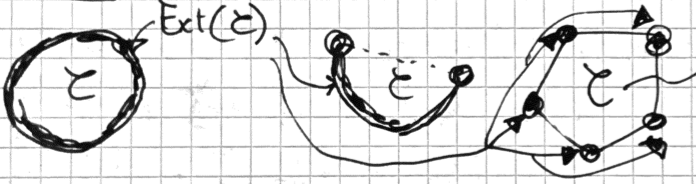
\includegraphics[width=.45\linewidth]{birkhoff/extremal-pts}&
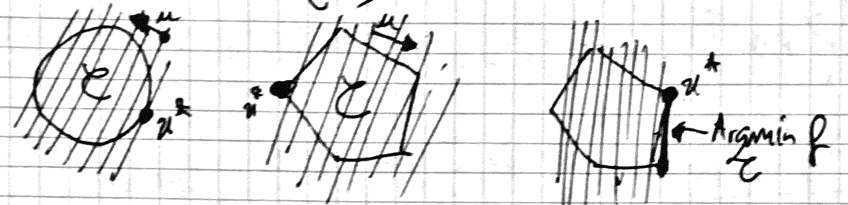
\includegraphics[width=.45\linewidth]{birkhoff/min-cvx}
\end{tabular}
\caption{\label{fig-extremal}
%
Left: extremal points of a convex set. 
Right: the solution of a convex program is a convex set. 
}
\end{figure}


\begin{prop}\label{prop-extr-optim}
	If $\Cc$ is compact, then 
	\eq{
		\text{Extr}(\Cc) \cap \pa{ \uargmin{\P \in \Cc} \dotp{\C}{\P}  } \neq \emptyset.
	}
\end{prop}
\begin{proof}
	One consider $\Ss \eqdef \uargmin{\P \in \Cc} \dotp{\C}{\P}$. 
	%	
	We first note that $\Ss$ is convex (as always for an argmin) and compact, because $\Cc$ is compact and the objective function is continuous, so that $\text{Extr}(\Ss) \neq \emptyset$.
	%
	We will show that $\text{Extr}(\Ss) \subset \text{Extr}(\Cc)$. 
	\todo{finish}
\end{proof}

The following theorem states that the extremal points of bistochastic matrices are the permutation matrices. It implies as a corollary that the cost of Monge and Kantorovitch are the same, and that they share a common solution. 


\begin{thm}[Birkhoff and von Neumann]\label{thm-birkh-vnm}
	One has $\text{Extr}(\Bb_n) = \Pp_n$.
\end{thm}
\begin{proof}
	We first show the simplest inclusion $\Pp_n \subset \text{Extr}(\Bb_n)$. Indeed it follows from the fact that $\text{Extr}([0,1]) = \{0,1\}$. Take $\P \in \Pp_n$, if $\P=(Q+R)/2$ with $Q_{i,j},R_{i,j} \in [0,1]$, since $\P_{i,j} \in \{0,1\}$ then necessarily $Q_{i,j}=R_{i,j} \in \{0,1\}$.
	
	Now we show $\text{Extr}(\Bb_n) \subset \Pp_n$ by showing that $\Pp_n^c \subset \text{Extr}(\Bb_n)^c$ where the complementary are computed inside the larger set $\Bb_n$. So picking $\P \in \Bb_n \backslash \Pp_n$, we need to split $\P = (Q+R)/2$ where $Q,R$ are distinct bistochastic matrices. 
	%
	As shown on figure~\ref{fig-extremal}, $\P$ defines a partite graph linking two sets of $n$ vertices. 
	%
	This graph is composed of isolated edge when $\P_{i,j}=1$ and connected edges corresponding to $0 < \P_{i,j} <1$.
	If $i$ is such a connected vertex on the left (similarly for $j$ on the right), because $\sum_j \P_{i,j}=1$, there is necessarily at least two edges $(i,j_1)$ and $(i,j_2)$ emating from it (similarely on the right there are at least two converging edges $(i_1,j)$ and $(i_2,j)$). This means that by following these connexions, one necessarily can extract a cycle (if not, one could alway extend it by the previous remarks) of the form
	\eq{
		(i_1,j_1,i_2,j_2,\ldots,i_p,j_p), 
		\quad \text{i.e.}\quad i_{p+1}=i_1.
	}
	We assume this cycle is the shortest one among all this (finite) ensemble of cycle. Along this cycle, the left-right and right-left edges satisfy
	\eq{
		0 < \P_{i_s,j_s}, \P_{j_s,i_{s+1}} < 1.
	}
	The $(i_s)_s$ and $(j_s)_s$ are also all distincts because the cycle is the shortest. Lets pick
	\eq{
		\epsilon \eqdef \umin{0 \leq s \leq p} \{ \P_{i_s,j_s}, \P_{j_s,i_{s+1}}, 1-\P_{i_s,j_s}, 1-P_{j_s,i_{s+1}} \}
	}
	so that $0 < \epsilon < 1$. As shown on Figure~\ref{fig-extremal}, right, we split the graph in two set of edges, left-right and right-left
	\eq{
		\Aa \eqdef \{(i_s,j_s)\}_{s=1}^p
		\qandq 
		\Bb \eqdef \{(j_s,i_{s+1})\}_{s=1}^p.
	}
	We define then two matrices as
	\eq{
		Q_{i,j} \eqdef 
		\choice{
			\P_{i,j} \qifq (i,j) \notin \Aa \cup \Bb, \\
			\P_{i,j}+\epsilon/2 \qifq (i,j) \in \Aa, \\
			\P_{i,j}-\epsilon/2 \qifq (i,j) \in \Bb, 		
		}
		\qandq
		R_{i,j} \eqdef 
		\choice{
			\P_{i,j} \qifq (i,j) \notin \Aa \cup \Bb, \\
			\P_{i,j}-\epsilon/2 \qifq (i,j) \in \Aa, \\
			\P_{i,j}+\epsilon/2 \qifq (i,j) \in \Bb, 		
		}.
	}
	Because of the choice of $\epsilon$, one has $0 \leq Q_{i,j}, R_{i,j} \leq 1$.
	Because each left-right edge in $\Aa$ is associated to a right-left edge in $\Bb$, (and the other way) the
	sum constraint on the row (and on the column) is maintain, so that $U,V \in \Bb_n$. Finally, note that $\P=(P+Q)/2$.	
\end{proof}



\begin{figure}
\centering
\begin{tabular}{@{}c@{\hspace{5mm}}c@{}}
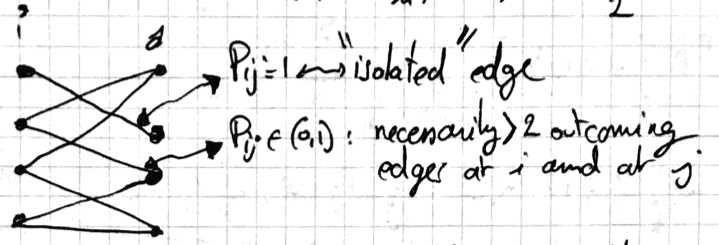
\includegraphics[width=.7\linewidth]{birkhoff/bipartite}&
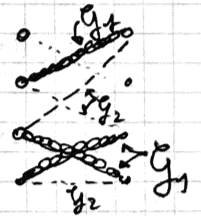
\includegraphics[width=.25\linewidth]{birkhoff/bipartite-split}
\end{tabular}
\caption{\label{fig-extremal}
%%
Left: the support of the coupling $\P$ defines a bipartite graph.
Right: splitting of this graph in two set of edges.
}
\end{figure}

By putting together Proposition~\ref{prop-extr-optim} and Theorem~\ref{thm-birkh-vnm}, one obtains that for the discrete optimal problem with empirical measures, Monge and Kantoritch problems are equivalent.

\begin{cor}[Kantorovich for matching]\label{prop-matching-kanto}
	If $m=n$ and $\a=\b=\ones_n$, then there exists an optimal solution for Problem~\eqref{eq-mk-discr} $\P_{\si^\star}$, which is a permutation matrix associated to an optimal permutation $\si^\star \in \Perm(n)$ for Problem~\eqref{eq-optimal-assignment}.	
\end{cor}

The following proposition shows that these problems result in fact in the same optimum, namely that one can always find a permutation matrix that minimizes Kantorovich's problem~\eqref{eq-mk-discr} between two uniform measures $\a=\b=\ones_n/n$, which shows that the Kantorovich relaxation is \emph{tight} when considered on assignment problems. %Note however that some computational algorithm, which are combinatorial in nature, are dedicated to the case of uniform histograms with the same number of points (see Chapter~\ref{c-algo-basics}). 
%
% Figure~\ref{fig-matching-kantorovitch} shows on the left a 2-D example of optimal matching corresponding to this special case. 

%\begin{figure}
%\centering
%\begin{tabular}{@{}c@{\hspace{5mm}}c@{}}
%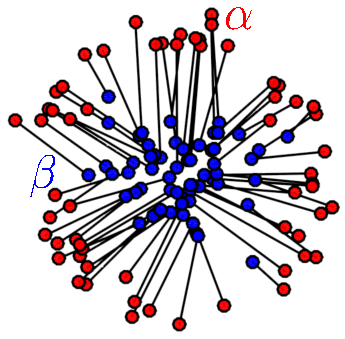
\includegraphics[width=.25\linewidth]{matching-kantorovitch/matching}&
%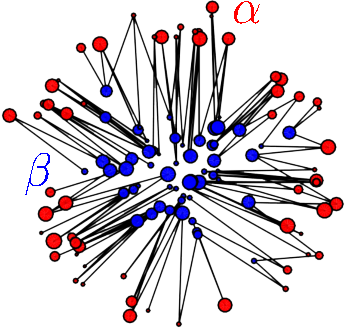
\includegraphics[width=.25\linewidth]{matching-kantorovitch/weighted}
%\end{tabular}
%\caption{\label{fig-matching-kantorovitch}
%%
%Comparison of optimal matching and generic couplings. A black segment between $x_i$ and $y_j$ indicates a non-zero element in the displayed optimal coupling $\P_{i,j}$ solving~\eqref{eq-mk-discr}.
%%
%Left: optimal matching, corresponding to the setting of Proposition~\eqref{prop-matching-kanto} (empirical measures with the same number $n=m$ of points).
%%
%Right: these two weighted point clouds cannot be matched; instead a Kantorovich coupling can be used to associate two arbitrary discrete measures.  
%}
%\end{figure}


\begin{rem}[General case] For general input measure, one does not have equivalence between Monge and Kantorovitch problems (since the Monge constraint is in general empty). But the support of the optimal coupling $\P$ still enjoys some strong regularity, in particular, it defines a cycle-free bipartite graph. This implies in particular that the resulting $\P$ matrix is sparse, for instance one can show that there are always solutions with less than $n+m-1$ non-zero elements.	
\end{rem}

%%%%%%%%%%%%%%%%%%%%%%%%%%%%%%%%%%%%%%%%%%%%%%%%%%%%%%%%%%%%%%%%%%%%%%%%%%%
\subsection{Relaxation for Arbitrary Measures}

%%%
\paragraph{Continuous couplings.}

The definition of $\MK_\c$ in~\eqref{eq-kanto-discr} is extended to arbitrary measures by considering couplings $\pi \in \Mm_+^1(\X \times \Y)$ which are joint distributions over the product space. 
%
The marginal constraint $\P\ones_m=\a, \P\ones_n=\b$ must be replaced by ``integrated'' versions, which are written $\pi_1 = \al$ and $\pi_2 = \be$, where $(\pi_1,\pi_2) \in \Mm(\Xx) \times \Mm(\Yy)$ are the two marginals. 
%
They are defined as $\pi_1 \eqdef P_{1\sharp} \pi$ and $\pi_2 \eqdef P_{2\sharp} \pi$ the two marginals of $\pi$, which are defined using push-forward by the projectors $P_1(x,y)=x$ and $P_2(x,y)=y$.

A heuristic way to understand the marginal constraint $\pi_1 = \al$ and $\pi_2 = \be$, which mimics the discrete case where one sums along the rows and columns is to write
\eq{
	\int_\Yy \d\pi(x,y) = \d\al(x)
	\qandq
	\int_\Xx \d\pi(x,y) = \d\be(y),
}
and the mathematically rigorous way to write this, which corresponds to the change of variables formula, is 
\eq{
	\foralls (f,g) \in \Cc(\Xx) \times \Cc(\Yy), \quad
	\int_{\Xx \times \Yy} f(x) \d\pi(x,y) = \int_\Xx f \d\al
	\qandq
	\int_{\Xx \times \Yy} \d\pi(x,y) = \int_\Yy g \d\be.
}	
%
Using~\eqref{eq-equiv-pushfwd}, these marginal constraints are also equivalent to imposing that $\pi(A \times \Y)=\al(A)$ and $\pi(\X \times B)=\be(B)$ for sets $A \subset \X$ and $B \subset \Y$.

Replacing continuous functions by indicator function, one can also rephrase this conservation of mass constraint as
\eq{
	\foralls (A,B) \in \X \times \Y, \quad
		\pi(A \times \Y) = \al(A)
		\qandq
		\pi(\X \times B) = \be(B). 
}

In the general case, the mass conservation constraint~\eqref{eq-discr-couplings} should thus rewritten as a marginal constraint on joint probability distributions
\eql{\label{eq-coupling-generic}
	\Couplings(\al,\be) \eqdef 
	\enscond{
		\pi \in \Mm_+^1(\X \times \Y)
	}{
		\pi_1 = \al
		\qandq
		\pi_2 = \be
	}.
} 

The discrete case, when $\al=\sum_i \a_i \de_{x_i}$, $\be=\sum_j \a_j \de_{x_j}$, the constraint $\pi_1=\al$ and $\pi_2=\be$ necessarily imposes that $\pi$ is discrete, supported on the set $\{(x_i,y_j)\}_{i,j}$, and thus has the form $\pi = \sum_{i,j} \P_{i,j} \de_{(x_i,y_j)}$. The discrete formulation is thus a special case (and not some sort of approximation) of the continuous formulation. 

The set $\Couplings(\al,\be)$ is always non-empty because it contains at least the tensor product coupling $\al \otimes \be$ defined by $\d(\al\otimes\be)(x,y)=\d\al(x)\d\be(y)$ i.e.
\eq{
	\foralls h \in \Cc(\Xx\times\Yy), \quad
	\int_{\X \times \Y} h(x,y)\d(\al\otimes\be)(x,y) = \int_\X (\int_\Y h(x,y) \d\be(y)) \d\al(x)
	=  \int_\X (\int_\Y h(x,y) \d\al(x) ) \d\be(y).
} 
Indeed, $(\al\otimes\be)_1 = \al$ since
\eq{
	\foralls f \in \Cc(\X), \quad
	\int_\X f(x) \d (\al\otimes\be)_1(x)
	= 
	\int_{\X \times \Y} f(x) d\al(x)\d\be(y)
	= \int_\X f(x) \d\al(x) \int_\Y \d\be
	= \int_\X f(x) \d\al(x)
}
because $\int_\Y \d\be=1$.

A very different (concentrated) type of coupling is defined when there exists a map $T: \X \rightarrow \Y$ such that $T_\sharp \al = \be$ (i.e. the constraint set of Monge's problem~\eqref{eq-monge-continuous} is non-empty). In this case, one has that $\pi = (\Id,T)_\sharp \al \in \Couplings(\al,\be)$. This coupling is defined though the integrated definition of push-forward as
\eq{
	\foralls h \in \Cc(\Xx\times\Yy), \quad
	\int_{\X \times \Y} h(x,y)\d\pi(x,y)
	= 
	\int_{\X} h(x,T(x))\d\al. 
} 
In particular, applying this formula to $h(x,y)=f(x)$ or $h(x,y)=g(y)$  shows that $\pi_1=\al$ and $\pi_2=\be$.



%
%
%\begin{figure}
%\centering
%\begin{tabular}{@{}c@{\hspace{5mm}}c@{\hspace{5mm}}c@{}}
%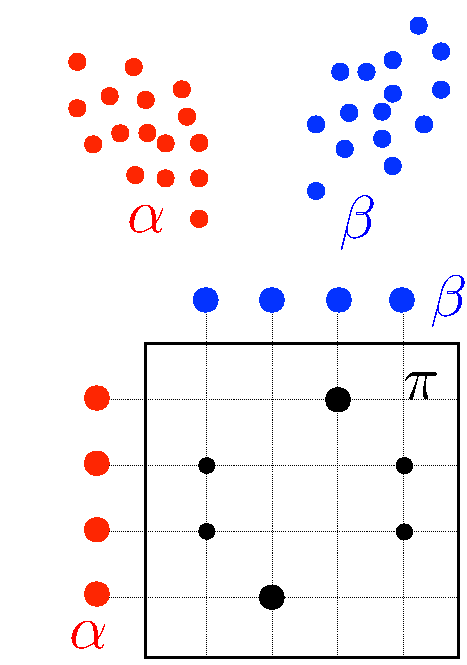
\includegraphics[width=.22\linewidth]{settings/discrete}&
%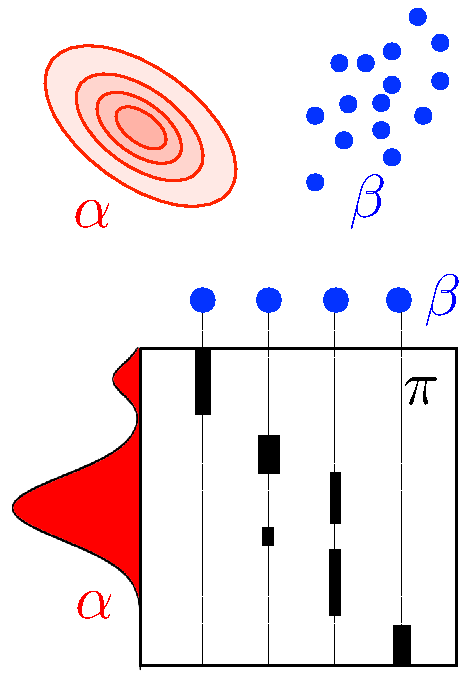
\includegraphics[width=.22\linewidth]{settings/semi-discrete}&
%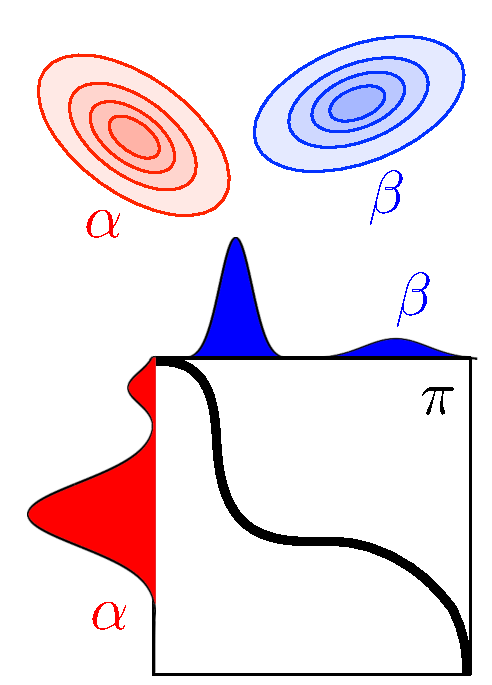
\includegraphics[width=.22\linewidth]{settings/continuous}\\
%Discrete & Semi-discrete & Continuous
%\end{tabular}
%\caption{\label{fig-settings}
%Schematic viewed of input measures $(\al,\be)$ and couplings $\Couplings(\al,\be)$ encountered in the three main scenario for Kantorovich OT. Chapter~\ref{c-algo-semidiscr} is dedicated to the semi-discrete setup.
%}
%\end{figure}


%%%
\paragraph{Continuous Kantorovitch problem.}


The Kantorovich problem~\eqref{eq-kanto-discr} is then generalized as 
\eql{\label{eq-mk-generic}
	\MK_\c(\al,\be) \eqdef 
	\umin{\pi \in \Couplings(\al,\be)}
		\int_{\X \times \Y} \c(x,y) \d\pi(x,y).
}
This is an infinite-dimensional linear program over a space of measures. 


% Figure~\ref{fig-couplings} shows examples of discrete and continuous optimal coupling solving~\eqref{eq-mk-generic}.
% Figure~\ref{fig-couplings-simple} shows other examples of optimal 1-D couplings, involving discrete and continuous marginals.

%\begin{figure}
%\centering
%\begin{tabular}{@{}c@{\hspace{10mm}}c@{}}
%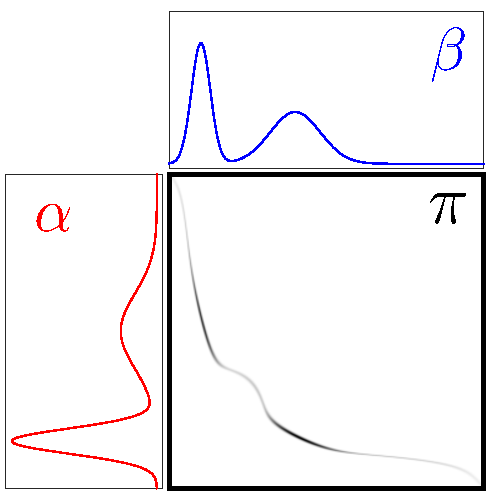
\includegraphics[width=.2\linewidth]{couplings/couplings-continuous}&
%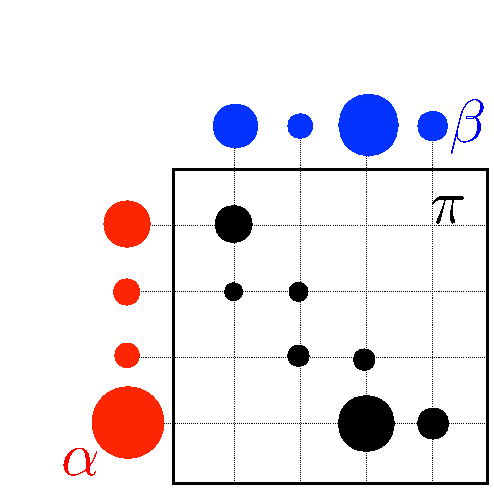
\includegraphics[width=.2\linewidth]{couplings/couplings-discr}
%\end{tabular}
%\caption{\label{fig-couplings}
%Left: ``continuous'' coupling $\pi$ solving~\eqref{eq-coupling-generic} between two 1-D measure with density. The coupling is localized along the graph of the Monge map $(x,\T(x))$ (displayed in black).  
%%
%Right: ``discrete'' coupling $\T$ solving~\eqref{eq-mk-discr} between two discrete measures of the form~\eqref{eq-pair-discr}. The non-zero entries $\T_{i,j}$  are display with a black disk at position $(i,j)$ with radius proportional to $\T_{i,j}$.
%}
%\end{figure}


%\begin{figure}
%\centering
%\begin{tabular}{@{}c@{}c@{}c@{}c@{}}
%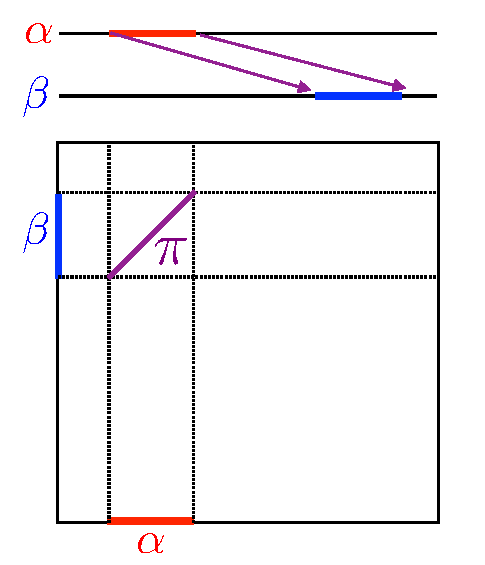
\includegraphics[width=.2\linewidth]{couplings/couplings-1}&
%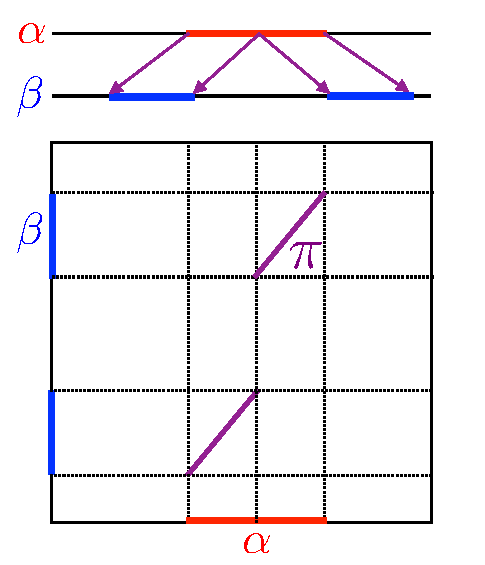
\includegraphics[width=.2\linewidth]{couplings/couplings-2}&
%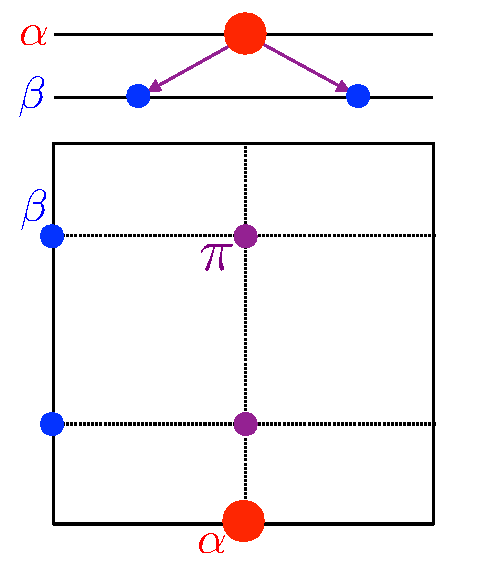
\includegraphics[width=.2\linewidth]{couplings/couplings-3}&
%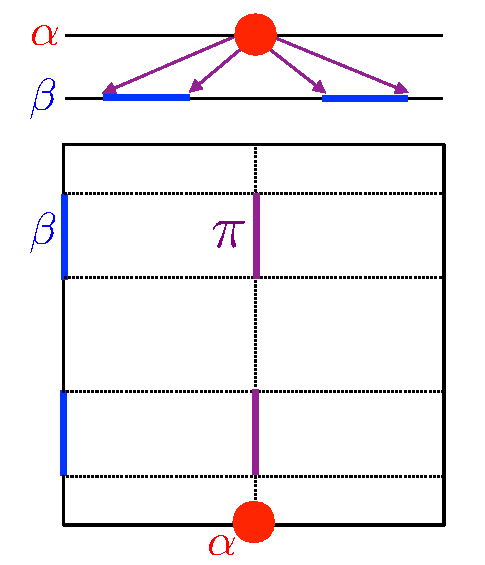
\includegraphics[width=.2\linewidth]{couplings/couplings-4}
%\end{tabular}
%\caption{\label{fig-couplings-simple}
%Four simple examples of optimal couplings between 1-D distributions, represented as maps above (arrows) and couplings below. Inspired by~\cite{Levy2017review}.
%}
%\end{figure}


On compact domain $(\Xx,\Yy)$, \eqref{eq-mk-generic} always has a solution, because using the weak-* topology (so called weak topology of measures), the set of measure is compact, and a linear function with a continuous $c(x,y)$ is weak-* continuous. And the set of constraint is non empty, taking $\al \otimes \be$. On non compact domain, one needs to impose moment condition on $\al$ and $\be$.

%%%%
\paragraph{Probabilistic interpretation.}

If we denote $X \sim \al$ the fact that the law of a random vector $X$ is the probability distribution $\al$, then the marginal constraint appearing in~\eqref{eq-mk-generic} is simply that $\pi$ is the law of a couple $(X,Y)$ and that its coordinates $X$ and $Y$ have laws $\al$ and $\be$. The coupling $\pi$ encodes the statistical dependency between $X$ and $Y$. For instance, $\pi = \al\otimes \be$ means that $X$ and $Y$ are independent, and it unlikely that such a coupling is optimal. Indeed as stated by Brenier's theorem, optimal coupling for a square Euclidean loss on contrary describe totally dependent variable, which corresponds to a coupling of the form $\pi=(\Id,T)_\sharp \al$ in which case $Y=T(X)$ where $T: \X \rightarrow \Y$ is a measurable map. 

With this remark, problem~\eqref{eq-mk-generic} reads equivalently 
\eql{\label{eq-mk-proba}
	\MK_\c(\al,\be) = 
	\umin{X \times \al, Y \sim \be} \EE(c(X,Y)).
}

%%%%
\paragraph{Monge-Kantorovitch equivalence.}

The proof of Brenier theorem~\ref{thm-brenier}  (detailed in Section~\ref{sec-c-transfo}, Remark~\ref{rem-proof-brenier}) to prove the existence of a Monge map actually studies Kantorovitch relaxation (and makes use of duality), and proves that this relaxation is tight in the sense that it has the same cost as Monge problem. 

Indeed, it shows that the support of an optimal $\pi$ is contained in the subdifferential $\partial \phi$ of a convex function $\phi$, which in general is a set-valued mapping \todo{give the example of a segment split into two equally spaced segments}.
%
When $\alpha$ does not have a density, then $\phi$ is non-smooth and non-smooth points where $\al(\{x\})>0$ leads to mass splitting, for instance moving $\de_{0}$ to $(\de_{-1}+\de{+1})/2$ can be achieved using $\phi(x)=|x|$.  


If $\al$ has a density, then this $\phi$ is differentiable $\al$-almost everywhere and we denote $\T=\nabla\phi$ the unique optimal transport (which is a valid definition almost everywhere and one can use any value at point of non differentiability), then the coupling 
\eq{
	\pi = (\Id,\T)_\sharp \al
	\quad\text{i.e.}\quad
	\foralls h \in \Cc(\Xx \times \Yy), \quad
	\int_{\Xx \times \Yy} h \d \pi = \int_{\Xx} h(x,\T(x)) \d\al(x)
}
is optimal.
In term of random vector, denoting $(X,Y)$ a random vector with law $\pi$, it means that any such optimal random vector satisfies $Y=\T(X)$ where $X \sim \al$ (and of course $\T(X) \sim \be$ by the marginal constraint). 


This key result is similar to Birkoff-von-Neumann Theorem~\ref{prop-matching-kanto} in the sense that it provides conditions ensuring the equivalence between Monge and Kantorovitch problems (note however that Birkoff-von-Neumann does not implies uniqueness). Note however that the settings are radically difference (one is fully discrete while the other requires the sources to  be ``continuous'', i.e. to have a density).


%%%%%%%%%%%%%%%%%%%%%%%%%%%%%%%%%%%%%%%%%%%%%%%%%%%%%%%%%%%%%%%%%%%%%%%%%%%
\subsection{Metric Properties}

%%%%
\paragraph{OT defines a distance.}

An important feature of OT is that it defines a distance between histograms and probability measures as soon as the cost matrix satisfies certain suitable properties. Indeed, OT can be understood as a canonical way to lift a ground distance between points to a distance between histogram or measures. 

% We first consider the case where, using a term first introduce by~\cite{RubTomGui00}, the ``ground metric'' matrix $\C$ is fixed, representing substitution costs between bins, and shared across several histograms we would like to compare. The following proposition states that OT provides a meaningful distance between histograms supported on these bins.

\begin{prop}\label{prop-metric-histo}
We suppose $n=m$, and that for some $p \geq 1$, $\C=\distD^p=(\distD_{i,j}^p)_{i,j} \in \RR^{n \times n}$ where $\distD \in \RR_+^{n \times n}$ is a distance on $\range{n}$, \emph{i.e.}
\begin{enumerate}% [label=(\roman*)]
	\item $\distD \in \RR_+^{n \times n}$ is symmetric; 
	\item $\distD_{i,j}=0$ if and only if $i=j$; 
	\item $\foralls (i,j,k) \in \range{n}^3, \distD_{i,k} \leq \distD_{i,j}+\distD_{j,k}$.
\end{enumerate}
Then 
\eql{\label{eq-wass-p-disc}
	\WassD_p(\a,\b) \eqdef \MKD_{\distD^p}(\a,\b)^{1/p}
}
(note that $\WassD_p$ depends on $\distD$) defines the $p$-Wasserstein distance on $\Si_n$, \emph{i.e.} $\WassD_p$ is symmetric, positive, $\WassD_p(\a,\b)=0$ if and only if $\a = \b$, and it satisfies the triangle inequality
\eq{
	\foralls \a,\a',\b \in \Si_n, \quad \WassD_p(\a,\b) \leq \WassD_p(\a,\a') + \WassD_p(\a',\b).
}
\end{prop}

\begin{proof}
Symmetry and definiteness of the distance are easy to prove: since $\C = \distD^p$ has a null diagonal, $\WassD_p(\a,\a)=0$, with corresponding optimal transport matrix $\P^\star=\diag(\a)$; by the positivity of all off-diagonal elements of $\distD^p$, $\WassD_p(\a,\b)>0$ whenever $\a\ne \b$ (because in this case, an admissible coupling necessarily has a non-zero element outside the diagonal); by symmetry of $\distD^p$, $\WassD_p(\a,\b)=0$ is itself a symmetric function. 


To prove the triangle inequality of Wasserstein distances for arbitrary measures, \cite[Theorem 7.3]{Villani03} uses the gluing lemma, which stresses the existence of couplings with a prescribed structure. 
% Closed forms for such couplings exist in the discrete case which we can readily use. 
In the discrete setting, the explicit constuction of this glued coupling is simple.
%
Let $\a,\b,\VectMode{c} \in\simplex_n$. Let $\P$ and $\Q$ be two optimal solutions of the transport problems between $\a$ and $\b$, and $\b$ and $\VectMode{c}$ respectively. 
%
We define $\bar\b_j \eqdef \b_j$ if $\b_j>0$ and set otherwise $\bar\b_j=1$ (or actually any other value). We then define 
\eq{
	\SS \eqdef \P \diag(1/\bar\b) \Q \in \RR_+^{n \times n}.
} 
We remark that $\SS \in \U(\a,\VectMode{c})$ because 
\eq{
	\SS \ones_n  = \P \diag(1/\bar\b) \Q \ones_n = \P (\b / \bar\b) = \P \ones_{\Supp(\b)} = \a
}
where we denoted $\ones_{\Supp(\b)}$ the indicator of the support of $\b$, and we use the fact that $\P \ones_{\Supp(\b)} = \P \ones = \b$ because necessarily $\P_{i,j} = 0$ for $j \notin \Supp(\b)$.
Similarly one verifies that $\SS^\top \ones_n = \VectMode{c}$.


The triangle inequality follows from
%   notice that $\SS_{i\cdot k}$ being therefore a matrix of $\U(\a,\b)$ we can write:
$$\begin{aligned}
\WassD_p(\a,\VectMode{c})&=\left(\min_{\P\in U(\a,\VectMode{c})}\dotp{\P}{\distD^p}\right)^{1/p} \leq \dotp{\SS}{\distD^p}^{1/p}\\
&= \left(\sum_{ik} \distD^p_{ik}\sum_{j} \frac{\P_{ij}\Q_{jk}}{\bar\b_j}\right)^{1/p} \leq \left(\sum_{ijk} \left(\distD_{ij}+\distD_{jk}\right)^p \frac{\P_{ij}\Q_{jk}}{\bar\b_j}\right)^{1/p} \\
& \leq \left(\sum_{ijk} \distD^p_{ij} \frac{\P_{ij}\Q_{jk}}{\bar\b_j}\right)^{1/p} + \left(\sum_{ijk}\distD^p_{jk} \frac{\P_{ij}\Q_{jk}}{\bar\b_j}\right)^{1/p} \\
&= \left(\sum_{ij} \distD^p_{ij}\P_{ij} \sum_k \frac{\Q_{jk}}{\bar\b_j}\right)^{1/p} + \left(\sum_{jk} \distD^p_{jk} \Q_{jk} \sum_i \frac{\P_{ij}}{\bar\b_j}\right)^{1/p}\\
&= \left(\sum_{ij} \distD^p_{ij}\P_{ij}\right)^{1/p} + \left(\sum_{jk} \distD^p_{jk} \Q_{jk}\right)^{1/p}\\ 
&= \WassD_p(\a,\b) +\WassD_p(\b,\b).
\end{aligned}
$$
%
The first inequality is due to the suboptimality of $\SS$, the second is the usual triangle inequality for elements in $\distD$, and the third comes from Minkowski's inequality.
\end{proof}

Proposition~\ref{prop-metric-histo} generalizes from histogram to arbitrary measures that need not be discrete.

\begin{prop}\label{prop-metric-measure}
We assume $\X=\Y$, and that for some $p \geq 1$, $\c(x,y)=\dist(x,y)^p$ where $\dist$ is a distance on $\X$, \emph{i.e.} \\
	\hbox{}\qquad (i) $\dist(x,y) = \dist(y,x) \geq 0$;  \\
	\hbox{}\qquad (ii)  $\dist(x,y)=0$ if and only if $x=y$;  \\
	\hbox{}\qquad (ii)  $\foralls (x,y,z) \in \X^3, \dist(x,z) \leq \dist(x,y)+\dist(y,z)$. \\
Then 
\eql{\label{eq-defn-wass-dist}
	\Wass_p(\al,\be) \eqdef \MK_{\dist^p}(\al,\be)^{1/p}
}
(note that $\Wass_p$ depends on $\dist$) defines the $p$-Wasserstein distance on $\X$, \emph{i.e.} $\Wass_p$ is symmetric, positive, $\Wass_p(\al,\be)=0$ if and only if $\al = \be$, and it satisfies the triangle inequality
\eq{
	\foralls (\al,\be,\ga) \in  \Mm_+^1(\X)^3, \quad \Wass_p(\al,\ga) \leq \Wass_p(\al,\be) + \Wass_p(\be,\ga).
}
\end{prop}

This distance $\Wass_p$ defined though Kantorovitch problem~\eqref{eq-defn-wass-dist} should be contrasted with the distance $\tilde\Wass$ obtained using Monge's problem~\eqref{eq-monge-distance}. Kantorovitch distance is always finite, while Monge's one might be infinite if the constraint set $\enscond{T}{T_\sharp \al=\be}$ is empty. In fact, one can show that as soon as this constraint set is non-empty, and even if no optimal $T$ exists, then one has $\Wass_p = \tilde\Wass_p$, which is a non-trivial result. Kantorovitch distance should thus be seen as a (convex) relaxation of Monge's distance, which behave in a much nicer way, as we will explore next (it is continuous with respect to the convergence in law topology.


%%%%
\paragraph{Convergence in law topology.}

Let us first note that on a compact space, all $W_p$ distance defines the same topology (although they are not equivalent, the notion of converging sequence is the same).

\begin{prop}\label{prop-comp-wass-p}
	On a compact space $\Xx$, one has for $p \leq q$
	\eq{
		W_p( \al,\be ) \leq W_q(\al,\be) \leq \text{\upshape diam}(\Xx)^{\frac{q-p}{q}} W_p(\al,\be)^{\frac{q}{p}}
	}
\end{prop}
\begin{proof}
	The left inequality follows from Jensen inequality, $\phi(\int c(x,y) \d\pi(x,y)) \leq \int \phi(c(x,y)) \d\pi(x,y)$, applied to any probability distribution $\pi$ and to the convex function $\phi(r)=r^{q/p}$ to $c(x,y)=\norm{x-y}^p$, so that one gets
	\eq{
		\pa{\int \norm{x-y}^{p} \d\pi(x,y)}^{\frac{q}{p}} \leq \int \norm{x-y}^{q} \d\pi(x,y).
	} 	
	The right inequality follows from
	\eq{
		\norm{x-y}^q \leq \text{diam}(\Xx)^{q-p} \norm{x-y}^p.
	}
\end{proof}

The Wasserstein distance $\Wass_p$ has many important properties, the most important one being that it is a weak distance, \emph{i.e.} it allows to compare singular distributions (for instance discrete ones) and to quantify spatial shift between the supports of the distributions. This corresponds to the notion of weak$^*$ convergence.

\begin{defn}[Weak$^*$ topology]\label{dfn-weak-conv}
	$(\al_k)_k$ converges weakly$^*$ to $\al$ in $\Mm_+^1(\Xx)$ (denoted $\al_k \rightharpoonup \al$) if and only if for any continuous function $f \in \Cc(\Xx)$, $\int_\Xx f \d\al_k \rightarrow \int_\Xx f \d\al$.
\end{defn}

In term of random vectors, if $X_n \sim \al_n$ and $X \sim \al$ (not necessarily defined on the same probability space), the weak$^*$ convergence corresponds to the convergence in law of $X_n$ toward $X$.

\begin{defn}[Strong topology]
The simplest distance on Radon measures is the total variation norm, which is the dual norm of the $L^\infty$ norm on $\Cc(\Xx)$ and whose topology is often called the ``strong'' topology
\eq{
	\norm{\al-\be}_{TV} \eqdef \usup{\norm{f}_\infty \leq 1} \int f \d(\al-\be)
	 = |\al-\be|(\Xx)
}
where $|\al-\be|(\Xx)$ is the mass of the absolute value of the difference measure. When $\al-\be=\rho \d x$ has a density, then $\norm{\al-\be}_{TV}=\int |\rho(x)| \d x=\norm{\rho}_{L^1(\d x)}$ is the $L^1$ norm associated to $\d x$. When $\al-\be=\sum_i u_i \de_{z_i}$ is discrete, then $\norm{\al-\be}_{TV}=\sum_i |u_i|=\norm{u}_{\ell^1}$ is the discrete $\ell^1$ norm. 
\end{defn}

In the special case of Diracs, having $\int f \d\de_{x_n} = f(x_n) \rightarrow \int f \d\de_{x} = f(x)$ for any continuous $f$ is equivalent to $x_n \rightarrow x$. One can then contrast the strong topology with the Wasserstein distance, if $x_n \neq x$, 
\eq{
	\norm{\de_{x_n}-\de_x}_{TV}=2
	\qandq
	W_p(\de_{x_n},\de_x) = d(x_n,x).
}
This shows that for the strong topology, Diracs never converge, while they do converge for the Wasserstein distance. In fact it is a powerful property of the Wasserstein distance, which is regular with respect to the weak$^*$ topology, and metrizes it.

\begin{prop}
	If $\Xx$ is compact, $\al_k \rightharpoonup \al$ if and only if $W_p(\al_k,\al) \rightarrow 0$. 
\end{prop}

The proof of this proposition requires the use of duality, and is delayed to later, see Proposition~\ref{cor-topol-wass}. 
On non-compact spaces, one needs also to impose the convergence of the moments up to order $p$.
%
Note that there exists alternative distances which also metrize weak convergence. The simplest one are Hilbertian kernel norms, which are detailed in Section~\ref{sec-dual-norms}.

Another example of such a weak convergence is the fact that on $\Xx=\RR$
\eq{
	\frac{1}{n} \sum_{k=1}^n \de_{k/n} \rightharpoonup \Uu_{[0,1]}
}
(convergence toward the uniform measure on $[0,1]$), which comes from the convergence of Riemann sums 
\eq{
	\foralls f \in \Cc(\RR), \quad
	\frac{1}{n} \sum_{k=1}^n f(k/n) \longrightarrow \int_0^1 f(x) \d x.
}
In contrary, one has that for all $n$, since the two measure are mutually singular
\eq{
	\norm{ \frac{1}{n} \sum_{k=1}^n \de_{k/n} - \Uu_{[0,1]}}_{TV} = 
	\norm{ \frac{1}{n} \sum_{k=1}^n \de_{k/n} }_{TV} +  \norm{\Uu_{[0,1]}}_{TV} = 2
}
so that there is no strong convergence. 


 
 
%%%%%
\paragraph{Applications and implications}

Applications for having a geometric distance : barycenters, shape registration loss functions, density fitting
% !TEX root = ../CourseOT.tex


%%%%%%%%%%%%%%%%%%%%%%%%%%%%%%%%%%%%%%%%%%%%%%%%%%%%%%%%%%%%%%%%%%%%%%%%%%%
%%%%%%%%%%%%%%%%%%%%%%%%%%%%%%%%%%%%%%%%%%%%%%%%%%%%%%%%%%%%%%%%%%%%%%%%%%%
%%%%%%%%%%%%%%%%%%%%%%%%%%%%%%%%%%%%%%%%%%%%%%%%%%%%%%%%%%%%%%%%%%%%%%%%%%%
\section{Sinkhorn}

%%%%%%%%%%%%%%%%%%%%%%%%%%%%%%%%%%%%%%%%%%%%%%%%%%%%%%%%%%%%%%%%%%%%%%%%%%%
\subsection{Entropic Regularization for Discrete Measures}


%%%%%
\paragraph{Relative entropy}

The Kullback-Leibler divergence is defined as
\eql{\label{eq-kl-defn}
	\KLD(\P|\Q) \eqdef \sum_{i,j}  \P_{i,j} \log\pa{\frac{\P_{i,j}}{\Q_{i,j}}} - \P_{i,j} + \Q_{i,j}.
}
with the convention $0\log(0)=0$ and $\KLD(\P|\Q)=+\infty$ if there exists some $(i,j)$ such that $\Q_{i,j}=0$ but $\P_{i,j} \neq 0$. 
%
The special case $\KLD(\P|\ones_{n \times m})$ corresponds to minus the Shannon-Boltzmann entropy
\eq{
	\HD( \P ) = -\KLD(\P|\ones_{n \times m}) = -\sum_{i,j} \P_{i,j} \log(\P_{i,j}). 
}
%
The function $\KLD(\cdot|\Q)$ is strongly convex, because its hessian is $\partial^2 \KLD(\P|\Q)=\diag(1/\P_{i,j})$ and $\P_{i,j} \leq 1$. 
%
Note that since in what follows $\P$ and $\Q$ are actually probability distributions, one has 
\eq{
	\KLD(\P|\Q) = \sum_{i,j}  \P_{i,j} \log\pa{\frac{\P_{i,j}}{\Q_{i,j}}},
} 
but considering the extra terms gives cleaner expressions, in particular $\nabla \KLD(\P|\Q) = \log(\P/\Q)$ and duality formula reads more nicely. And for later, it will be important to have this normalization when considering unbalanced OT (see Section~\ref{sec-unbalanced}).

$\KL$ is a particular instance (and actually the unique case) of both a $\phi$-divergence (as defined in Section~\ref{sec-phi-div}) and a Bregman divergence. This unique property is at the heart of the fact that this regularization leads to elegant algorithms and a tractable mathematical analysis. One thus has $\KLD(\P|\Q) \geq 0$ and  $\KLD(\P|\Q)=0$ if and only if $\P=\Q$ (see Proposition~\ref{phi-div-positive}).


%%%%%
\paragraph{Entropic Regularization for Discrete Measures.}

The idea of the entropic regularization of optimal transport is to use $\KLD$ as a regularizing function to obtain approximate solutions to the original transport problem~\eqref{eq-mk-discr}:
\eql{\label{eq-regularized-discr}
	\MKD_\C^\epsilon(\a,\b) \eqdef 
	\umin{\P \in \CouplingsD(\a,\b)}
		\dotp{\P}{\C} + \epsilon \KLD(\P|\a \otimes \b). 
} 
Here we used as a reference measure for the relative entropy $\a \otimes \b = (\a_i \b_j)_{i,j}$.
%
This choice of normalization, specially in this discrete setting, has no importance for the selection of the optimal $\P$ since it only affects the objective by a constant, as shown in the following proposition.

\begin{prop} For $\P \in \CouplingsD(\a,\b)$, one has
\eq{
	\KLD(\P|\a \otimes \b) = 
	\KLD(\P|\a' \otimes \b') - \KLD(\a|\a') - \KL(\b|\b').
} 
\end{prop}

\begin{proof}
This follows from 
\eq{
	\sum_{i,j} \P_{i,j} \log\frac{\P_{i,j}}{\a_i\b_j}
	= 
	\sum_{i,j} \P_{i,j} \log\frac{\P_{i,j}}{\a_i'\b_j'}
	+ 
	\sum_{i,j} \P_{i,j} \pa{\log\frac{\a_i'}{\a_i} + \log\frac{\b_j'}{\b_j}}.
} 
\end{proof}

In the case where $\a_i>0$ and $\b_j>0$ (full support histogram), one could thus replace the reference measure $\a \otimes \b$ by $\ones_{n \times m}$, and thus regularize using the penalty $\HD(\P)$ in place of $\KL(\P|\a \otimes \b)$, resulting in the same solution.
%
The choice of using the reference measure $\a \otimes \b$ is however important to deal with situation where the support of $\a$ and $\b$ can change (so that some coordinate of $\a$ or $\b$ might vanish), and more importantly in the following section which dealds with possibly continuous distributions. Note that it also affect the values of the cost $\MKD_\C^\epsilon(\a,\b)$.


% Figure~\ref{fig-impact-eps} illustrates the effect of the entropy to regularize a linear program over the simples $\simplex_3$ (which can thus be visualized as a triangle in 2-D). Note how the entropy pushes the original LP solution away from the boundary of the triangle. The optimal $\P_\epsilon$ progressively moves toward an ``entropic center'' of the triangle. This is further detailed in the proposition below. The convergence of the solution of that regularized problem towards an optimal solution of the original linear program has been studied by~\cite{CominettiAsympt}.


%\begin{figure}
%\centering
%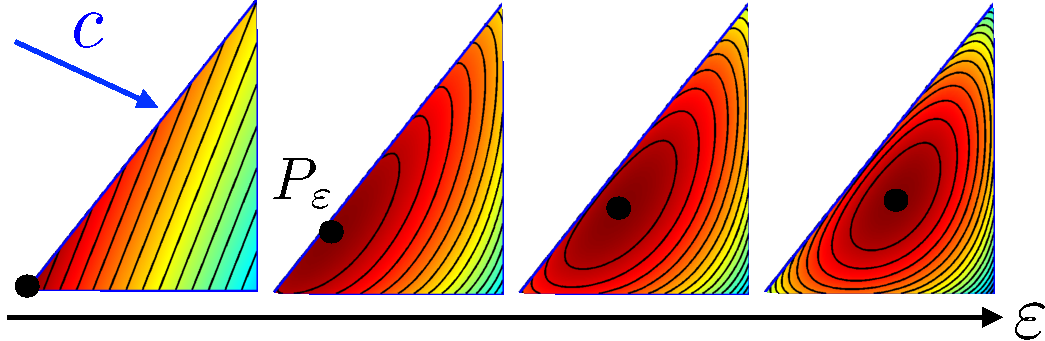
\includegraphics[width=.5\linewidth]{entropic/simplex}
%\caption{\label{fig-impact-eps}
%Impact of $\epsilon$ on the optimization of a linear function on the simplex, solving $\P_\epsilon = \argmin_{\P \in \simplex_3} \dotp{\C}{\P}-\epsilon\HD(\P)$ for a varying $\epsilon$. 
%}
%\end{figure}


%%%%%
\paragraph{Smoothing effect.}

Since the objective is a $\epsilon$-strongly convex function, problem~\ref{eq-regularized-discr} has a unique optimal solution. 
%
As studied in Section~\ref{}, this smoothing, beyond providing uniqueness, actually leads to $\MKD_\C^\epsilon(\a,\b)$ being a smooth function of $\a, \b$ and $\C$. 
%
The effect of the entropy is to act as a barrier function for the positivity constraint. As we will show next, this forces the solution $\P$ to be strictly positive on the support of $\a \otimes \b$. 

One has the following convergence property.
 
 
\begin{prop}[Convergence with $\epsilon$]\label{prop-convergence-eps}
The unique solution $\P_\epsilon$ of~\eqref{eq-regularized-discr} converges to the optimal solution with maximal entropy within the set of all optimal solutions of the Kantorovich problem, namely
\eql{\label{eq-entropy-conv-1}
	\P_\epsilon \overset{\epsilon \rightarrow 0}{\longrightarrow}
	\uargmin{\P} \enscond{ \KLD(\P|\a \otimes \b) }{
		\P \in \CouplingsD(\a,\b), \dotp{\P}{\C} = \MKD_\C(\a,\b)
	}
}
so that in particular
\eq{
	\MKD_\C^\epsilon(\a,\b) \overset{\epsilon \rightarrow 0}{\longrightarrow} \MKD_\C(\a,\b).
}
One has
\eql{\label{eq-entropy-conv-2}
	\P_\epsilon \overset{\epsilon \rightarrow \infty}{\longrightarrow}
	\a \otimes \b.
}
\end{prop}

\begin{proof}
	\textbf{Case $\epsilon \rightarrow 0$.}
	 We consider a sequence $(\epsilon_\ell)_\ell$ such that $\epsilon_\ell \rightarrow 0$ and $\epsilon_\ell > 0$.	
 	We denote $\P_\ell$ the solution of~\eqref{eq-regularized-discr} for $\epsilon=\epsilon_\ell$. 
	%
	Since $\CouplingsD(\a,\b)$ is bounded, we can extract a sequence (that we do not relabel for sake of simplicity) such that $\P_\ell \rightarrow \P^\star$. Since $\CouplingsD(\a,\b)$ is closed, $\P^\star \in \CouplingsD(\a,\b)$. We consider any $\P$ such that $\dotp{\C}{\P} = \MKD_\C(\a,\b)$. By optimality of $\P$ and $\P_\ell$ for their respective optimization problems (for $\epsilon=0$ and $\epsilon=\epsilon_\ell$), one has
 	\eql{\label{eq-proof-gamma-conv}
 		0 \leq \dotp{\C}{\P_\ell} - \dotp{\C}{\P} \leq \epsilon_\ell ( \KLD(\P_\ell|\a \otimes \b)-\KLD(\P|\a \otimes \b) ).
 	}
 	Since $\HD$ is continuous, taking the limit $\ell \rightarrow +\infty$ in this expression shows that 
 	$\dotp{\C}{\P^\star} = \dotp{\C}{\P}$ so that $\P^\star$ is a feasible point of~\eqref{eq-entropy-conv-1}. Furthermore, dividing by $\epsilon_\ell$ in~\eqref{eq-proof-gamma-conv} and taking the limit shows that 
 	$\KLD(\P|\a \otimes \b) \leq \KLD(\P^\star|\a \otimes \b)$, which shows that $\P^\star$ is a solution of~\eqref{eq-entropy-conv-1}. Since the solution $\P_0^\star$ to this program is unique by strict convexity of $\KLD(\cdot|\a \otimes \b)$, one has $\P^\star = \P_0^\star$, and the whole sequence is converging. 
	
	
	\textbf{Case $\epsilon \rightarrow +\infty$.} Evaluating at $\a \otimes \b$ the energy, one has
	\eq{
		\dotp{\C}{\P_\epsilon} + \epsilon \KLD(\P_\epsilon|\a \otimes \b) \leq \dotp{\C}{\a \otimes \b} + \epsilon \times 0
	}
	and since $\dotp{\C}{\P_\epsilon} \geq 0$, this leads to
	\eq{
		\KLD(\P_\epsilon|\a \otimes \b) \leq \epsilon^{-1} \dotp{\C}{\a \otimes \b} \leq \frac{\norm{\C}_\infty}{\epsilon}
	}
	so that $\KLD(\P_\epsilon|\a \otimes \b) \rightarrow 0$ and thus $\P_\epsilon \rightarrow \a \otimes \b$ since $\KLD$ is a valid divergence.
\end{proof}


%\begin{figure}
%\centering
%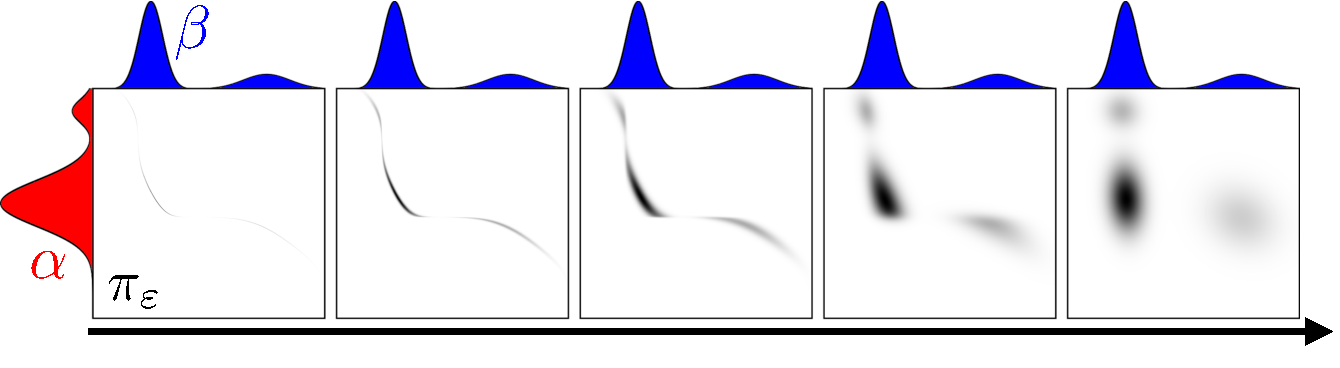
\includegraphics[width=.48\linewidth]{entropic/densities}
%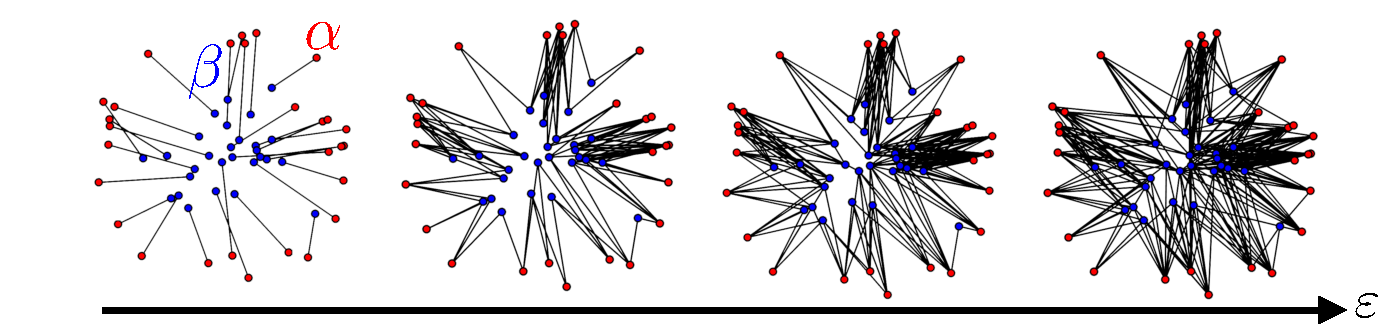
\includegraphics[width=.48\linewidth]{entropic/matching-2d}
%\caption{\label{fig-entropic}
%Impact of $\epsilon$ on coupling between densities and discrete distributions, illustrating Proposition~\ref{prop-convergence-eps}.
%%
%Left: between two 1-D densities. Right: between two 2-D discrete empirical densities with same number $n=m$ of points (only entries of the optimal $(\P_{i,j})_{i,j}$ above a small threshold are displayed as segments between $x_i$ and $y_j$).
%}
%\end{figure}




% \todo{First order expansion}


%%%%%%%%%%%%%%%%%%%%%%%%%%%%%%%%%%%%%%%%%%%%%%%%%%%%%%%%%%%%%%%%%%%%%%%%%%%
\subsection{General Formulation}

One can consider arbitrary measures by replacing the discrete entropy by the relative entropy with respect to the product measure $\d\al\otimes\d\be(x,y) \eqdef \d\al(x)\d\be(y)$, and propose a regularized counterpart to~\eqref{eq-mk-generic} using
\eql{\label{eq-entropic-generic}
	\MK_\c^\epsilon(\al,\be) \eqdef 
	\umin{\pi \in \Couplings(\al,\be)}
		\int_{X \times Y} c(x,y) \d\pi(x,y) + \epsilon \KL(\pi|\al\otimes\be)
}
where the relative entropy is a generalization of the discrete Kullback-Leibler divergence~\eqref{eq-kl-defn}
\eql{\label{eq-defn-rel-entropy}
	\KL(\pi|\xi) \eqdef \int_{\X \times \Y} \log\Big( \frac{\d \pi}{\d\xi}(x,y) \Big) \d\pi(x,y)
	  + \int_{\X \times \Y} (\d\xi(x,y)-\d\pi(x,y)), 
}
and by convention $\KL(\pi|\xi)=+\infty$ if $\pi$ does not have a density $\frac{\d \pi}{\d\xi}$ with respect to $\xi$. 
%
It is important to realize that the reference measure $\al\otimes\be$ chosen in~\eqref{eq-entropic-generic} to define the entropic regularizing term $\KL(\cdot|\al\otimes\be)$ plays no specific role, only its support matters.
%
This problem is often referred to as the ``static Schr\"odinger problem'', since $\pi$ is intended to model the most likely coupling between particules of gaz which can be only observed at two different times (it is the so-called lazy gaz model). The parameter $\epsilon$ controls the temperature of the gaz, and particules do not move in deterministic straight line as in optimal transport for the Euclidean cost, but rather according to a stochastic Brownian bridge. 

%Formula~\eqref{eq-entropic-generic} can be re-factored as a projection problem
% \eql{\label{eq-entropic-generic-proj}
%	\umin{\pi \in \Couplings(\al,\be)} \KL(\pi|\Kk)
% }
% where $\Kk$ is the Gibbs distributions $\d\Kk(x,y) \eqdef e^{-\frac{c(x,y)}{\epsilon}} \d\mu(x)\d\nu(y)$.
%
% This problem is often referred to as the ``static Schr\"odinger problem''~\cite{LeonardSchroedinger,RuschendorfThomsen}, since it was initially considered by Schr\"odinger in statistical physics~\cite{Schroedinger31}. 
%
% As $\epsilon \rightarrow 0$, the unique solution to~\eqref{eq-entropic-generic-proj} converges to the maximum entropy solution to~\eqref{eq-mk-generic}, see~\cite{leonard2012schrodinger,2017-carlier-SIMA}.
%
% ~\S\ref{sec-entropic-dynamic} details an alternate ``dynamic'' formulation of the Schr\"odinger problem over the space of paths connecting the points of two measures.

\begin{rem}[Probabilistic interpretation]
	If $(X,Y) \sim \pi$ have marginals $X \sim \al$ and $Y \sim \be$, then $\KL(\pi|\al \otimes \be) = \Ii(X,Y)$ is the mutual information of the couple, which is 0 if and only if $X$ and $Y$ are independent. The entropic problem~\eqref{eq-entropic-generic} is thus equivalent to
	\eq{
		\umin{(X,Y), X \sim \al, Y \sim \be } \EE( c(X,Y)) + \epsilon \Ii(X,Y). 
	}
	Using a large $\epsilon$ thus enforces the optimal coupling to describe independent variables, while, according to Brenier's theorem, small $\epsilon$ rather imposes a deterministic dependency between the couple according to a Monge map. 
\end{rem}

% - Probabilistic interpretation, mutual information, independence

%%%%%%%%%%%%%%%%%%%%%%%%%%%%%%%%%%%%%%%%%%%%%%%%%%%%%%%%%%%%%%%%%%%%%%%%%%%
\subsection{Sinkhorn's Algorithm}

The following proposition shows that the solution of~\eqref{eq-regularized-discr} has a specific form, which can be parameterized using $n+m$ variables. That parameterization is therefore essentially dual, in the sense that a coupling $\P$ in $\CouplingsD(\a,\b)$ has $nm$ variables but $n+m$ constraints.

\begin{prop}\label{prop-regularized-primal}
$\P$ is the unique solution to~\eqref{eq-regularized-discr} if and only if there exists  $(\uD,\vD) \in \RR_+^n \times \RR_+^m$ such that 
\eql{\label{eq-scaling-form}
	\foralls (i,j) \in \range{n} \times \range{m}, \quad \P_{i,j} = \uD_i \K_{i,j} \vD_j
	\qwhereq \K_{i,j} \eqdef e^{-\frac{-\C_{i,j}}{\epsilon}}, 
}
and $\P \in \Couplings(\a,\b)$.
\end{prop} 

\begin{proof} 
Without loss of generality, we assume $\a_i,\b_j>0$ (otherwise, we can set the corresponding $\uD_i$ or $\vD_j$ to 0).

The first thing to prove is that if $\P^\star$ is the solution (which is unique by strict convexity of the entropy) then $\P_{i,j}^\star>0$ for all $(i,j)$. Indeed, if $\P_{i,j}^\star=0$, then we can consider $\P_t = (1-t)\P^\star + t \a \otimes \b$, which satisfies the marginal constraint for $t \in [0,1]$. One then check that, denoting $\Ee(\P) \eqdef \dotp{\P}{\C}+\KLD(\P|\a \otimes \b)$ the objective function, and $f(t) \eqdef \Ee(\P_t)$, then $f'(0) = -\infty$, so that for $t$ small enough, $\Ee(\P_t)<\Ee(\P^\star)$ which is a contradiction.

We can thus ignore the positivity constraint when introducing two dual variables $\fD\in\RR^n,\gD\in\RR^m$ for each marginal constraint, so that the Lagrangian of~\eqref{eq-regularized-discr} reads
\eq{\label{eq-sinkhorn-lagrangian}
	\Lag(\P,\fD,\gD)= \dotp{\P}{\C} + \epsilon \KLD(\P|\a \otimes \b) + \dotp{\fD}{\a - \P\ones_m} + \dotp{\gD}{\b - \transp{\P}\ones_n}.
}
Considering first order conditions (where we ignore the positivity constraint, which can be made rigorous by showing the associated multiplier vanishes), we have
$$
	\frac{\partial\Lag(\P,\fD,\gD)}{\partial \P_{i,j}}= \C_{i,j} + \epsilon \log\pa{\frac{\P_{i,j}}{\a_i \b_j}} - \fD_i -\gD_j = 0.
$$
which results, for an optimal $\P$ coupling to the regularized problem, in the expression 
$\P_{i,j}=\a_i \b_j e^{\frac{\fD_i+\gD_j - \C_{i,j}}{\epsilon}}$ 
which can be rewritten in the form provided in the proposition using non-negative vectors $\uD \eqdef (\a_i e^{\fD_i/\varepsilon})_i$ and $\vD \eqdef (\b_j e^{\gD_j/\varepsilon})_j$.
\end{proof} 

The factorization of the optimal solution exhibited in Equation~\eqref{eq-scaling-form} can be conveniently rewritten in matrix form as $\P=\diag(\uD)\K\diag(\vD)$.
%
$\uD,\vD$ must therefore satisfy the following non-linear equations which correspond to the mass conservation constraints inherent to $\CouplingsD(\a,\b)$,
\eql{\label{eq-dualsinkhorn-constraints}
	\diag(\uD)\K\diag(\vD)\ones_m=\a,
	\qandq
	\diag(\vD)\K^\top \diag(\uD)\ones_n=\b,
}
These two equations can be further simplified, since $\diag(\vD)\ones_m$ is  $\vD$, and the multiplication of $\diag(\uD)$ times $\K \vD$ is 
\eql{\label{eq-dualsinkhorn-constraints2}
	\uD \odot (\K \vD) = \a
	\qandq
	\vD \odot (\transp{\K}\uD) = \b
}
where $\odot$ corresponds to entry-wise multiplication of vectors. That problem is known in the numerical analysis community as the matrix scaling problem (see~\cite{nemirovski1999complexity} and references therein).
%
An intuitive way to try to solve these equations is to solve them iteratively, by modifying first $\uD$ so that it satisfies the left-hand side of Equation~\eqref{eq-dualsinkhorn-constraints2} and then $\vD$ to satisfy its right-hand side. These two updates define Sinkhorn's algorithm
\eql{\label{eq-sinkhorn}	
	\itt{\uD} \eqdef \frac{\a}{\K \it{\vD}}
	\qandq
	\itt{\vD} \eqdef \frac{\b}{\transp{\K}\itt{\uD}},
}
initialized with an arbitrary positive vector, for instance $\init{\vD} = \ones_m$. The division operator used above between two vectors is to be understood entry-wise. Note that a different initialization will likely lead to a different solution for $\uD,\vD$, since $\uD,\vD$ are only defined up to a multiplicative constant (if $\uD,\vD$ satisfy \eqref{eq-dualsinkhorn-constraints} then so do $\lambda\uD,\vD/\lambda$ for any $\lambda>0$).
%
It turns out however that these iterations converge, as we detail next. 

\todo{Say a few word about the general probleme of scaling a matrix to a bistochastic one, and why this is non trivial for matrices with vanishing entries.}

%  (see Remark~\ref{rem-iterative-projection} for a justification using iterative projections, and Remark~\ref{rem-global-conv-sinkh} for a strict contraction result) and all result in the same optimal coupling $\diag(\uD)\K\diag(\vD)$. 
%
% Figure~\ref{fig-sinkhorn-convergence}, top row, shows the evolution of the coupling $\diag(\it{\UD})\K\diag(\it{\VD})$ computed by Sinkhorn iterations. It  evolves from the Gibbs kernel $\K$ towards the optimal coupling solving~\eqref{eq-regularized-discr} by progressively shifting the mass away from the diagonal.

%
%\begin{figure}
%\centering
%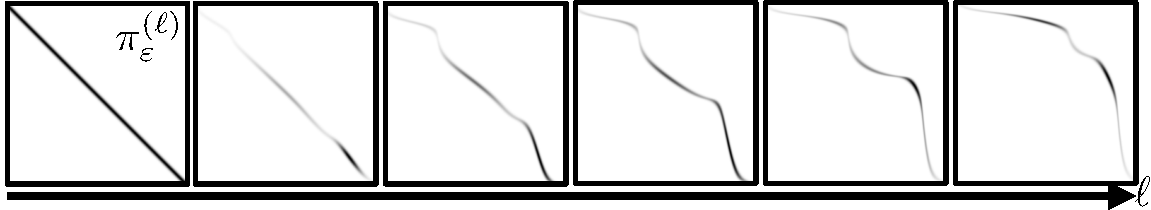
\includegraphics[width=.7\linewidth]{entropic/sinkhorn-convergence}
%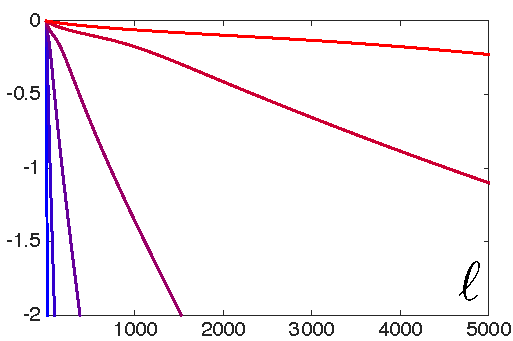
\includegraphics[width=.28\linewidth]{entropic/sinkhorn-rates}
%\caption{\label{fig-sinkhorn-convergence}
%Left: evolution of the coupling $\pi_\epsilon^\ell=\diag(\it{\UD})\K\diag(\it{\VD})$ computed at iteration $\ell$ of Sinkhorn's iterations, for 1-D densities.
%Right: impact of $\epsilon$ the convergence rate of Sinkhorn, as measured in term of marginal constraint violation $\log( \norm{\pi_\epsilon^\ell \ones_m - \b}_1 )$.
%}
%\end{figure}

A chief advantage, beside its simplicity, of Sinkhorn's algorithm is that the only computationnaly expensive step are matrix-vector multiplication by the Gibbs kernel, so that its complexity scales likes $Knm$ where $K$ is the number of Sinkhorn iteration, which can be kept polynomially in $1/\epsilon$ if one is interested in reaching an accuracy $\epsilon$ on the (unregularized) transportation cost. Note however that in many situation, one is not interested in reaching high accuracy, because targeted application success is often only remotely connected to the ability to solve an optimal transport problem (but rather only being able to compare in a geometrically faithful way distribution), so that $K$ is usually quite small.
%
This should be contrasted with interior point methods, which also operate by introducing a barrier function of the form $-\sum_i \log(\P_{i,j})$. These algorithm have typically a complexity of the order $O(n^6 \log(|\epsilon|))$ \todo{check}. 

The second crucial aspect of Sinkhorn is that matrix-vector multiplication streams extremely well on GPU. Even better, if one is interested in computing many OT problem with a fixed cost matrix $\C$, one can replace many matrix-vector multiplication by matrix-matrix multiplication, so that the computation gain is enormous. 


%%%%%%%%%%%%%%%%%%%%%%%%%%%%%%%%%%%%%%%%%%%%%%%%%%%%%%%%%%%%%%%%%%%%%%%%%%%
\subsection{Convergence}
\label{sec-convergence-init}

This section provides a first overview of convergence proof for Sinkhorn. For the sake of simplicity, this section is written for discrete measures, but the analysis caries over to general measure. This analysis is revisited in Section~\ref{} using convex duality. 

%%%%
\paragraph{Alternating $\KL$ projections.}

One has 
\eq{
	\dotp{\P}{\C} + \epsilon \KLD(\P|\a \otimes \b) = \epsilon \KLD(\P|\K) + \text{cst}, 
}
so that the unique solution $\P_\epsilon$ of~\eqref{eq-regularized-discr} is a projection onto $\CouplingsD(\a,\b)$ of the Gibbs kernel $\K$
\eql{\label{eq-kl-proj}
	\P_\epsilon = \Proj_{\CouplingsD(\a,\b)}^\KLD(\K) \eqdef \uargmin{\P \in \CouplingsD(\a,\b)} \KLD(\P|\K).
}

Denoting 
\eq{
	\Cc^1_\a \eqdef \enscond{\P}{\P\ones_m=\a}
	\qandq
	\Cc^2_\b \eqdef \enscond{\P}{\transp{\P}\ones_m=\b}
}
the rows and columns constraints, one has $\CouplingsD(\a,\b) = \Cc^1_\a \cap \Cc^2_\b$. One can use Bregman iterative projections~\cite{bregman1967relaxation}
\eql{\label{eq-kl-sinkh-proj}
	\itt{\P} \eqdef \Proj_{\Cc^1_\a}^{\KLD}(\it{\P})
	\qandq
	\ittt{\P} \eqdef \Proj_{\Cc^2_\b}^{\KLD}(\itt{\P}).
}
Since the sets $\Cc^1_\a$ and $\Cc^2_\b$ are affine, these iterations are known to converge to the solution of~\eqref{eq-kl-proj}, see~\cite{bregman1967relaxation}. 

The two projector are simple to compute since they corresponds to scaling respectively the rows and the columns
\eq{
	 \Proj_{\Cc^1_\a}^{\KLD}(\P) = \diag\pa{\frac{\a}{\P \ones_m}} \P
	 \qandq
	 \Proj_{\Cc^2_\b}^{\KLD}(\P) =  \P \diag\pa{\frac{\b}{\P^\top \ones_n}}.
}

These iterate are equivalent to Sinkhorn iterations~\eqref{eq-sinkhorn} since defining 
\eq{\label{eq-sink-matrix}\P^{(2\ell)} \eqdef \diag(\it{\uD}) \K \diag(\it{\vD}),}
one has
\begin{align*}
	\P^{(2\ell+1)} &\eqdef \diag(\itt{\uD}) \K \diag(\it{\vD}) \\
	\qandq
	\P^{(2\ell+2)} &\eqdef \diag(\itt{\uD}) \K \diag(\itt{\vD})
\end{align*}
In practice however one should prefer using~\eqref{eq-sinkhorn} which only requires manipulating scaling vectors and multiplication against a Gibbs kernel, which can often be accelerated (see below Remarks~\ref{rem-separable} and~\ref{rem-geod-heat}). 

Such a convergence analysis using Bregman projection is however of limited interested because it only works in finite dimension. For instance, the linear convergence speed one can obtain with these analyses (because the objective is strongly convex) will degrade with the dimension (and of course also with $\epsilon$). 
%
It is also possible to decay $\epsilon$ during the iterates to improve the speed and rely on multiscale strategies in low dimension.
 
% \todo{Remark on Bregman divergence, generalizatiton of projected gradient desc (mirror descent), etc.}



%%%%
\paragraph{Convergence for the Hilbert metric}

As initially explained by~\cite{franklin1989scaling}, the global convergence analysis of Sinkhorn is greatly simplified using Hilbert projective metric on $\RR_{+,*}^n$ (positive vectors), defined as
\eq{
	\foralls (\uD,\uD') \in (\RR_{+,*}^n)^2, \quad
	\Hilbert(\uD,\uD') \eqdef 
	\norm{\log(\uD)-\log(\vD)}_V
	% \log \umax{i,i'} \frac{ \uD_i \uD_{i'}' }{ \uD_{i'} \uD_{i}'  }.
}
where the variation semi-norm is
\eq{
	\norm{z}_V = \max(z)-\min(z).
}
One can show that $d_\Hh$ is a distance on the projective cone $\RR_{+,*}^n/\sim$, where $\uD \sim \uD'$ means that $\exists s>0, \uD=s\uD'$ (the vector are equal up to rescaling, hence the naming ``projective''), and that $(\RR_{+,*}^n/\sim,d_\Hh)$ is then a complete metric space.  
%
% This is a projective version of Hilbert's original distance on bounded open convex sets~\cite{hilbert1895gerade}.
%
It was introduced independently by~\cite{birkhoff1957extensions} and~\cite{samelson1957perron} to provide a quantitative proof of Perron-Frobenius theorem (convergence of iterations of positive matrices). Sinkhorn should be thought as a non-linear generalization of Perron-Frobenius. 

% , which, as explained in Remark~\ref{rem-local-conv} is linked to a local linearization of Sinkhorn's iterates. They proved the following fundamental theorem, which shows that a positive matrix is a strict contraction on the cone of positive vectors.

\begin{thm}\label{thm-birkoff}
	Let $\K \in \RR_{+,*}^{n \times m}$, then for $(\vD,\vD') \in (\RR_{+,*}^m)^2$
	\eq{
		\Hilbert(\K \vD,\K \vD') \leq \la(\K) \Hilbert(\vD,\vD')
		\text{ where }
		\choice{
			\la(\K) \eqdef \frac{ \sqrt{\eta(\K)}-1 }{ \sqrt{\eta(\K)}+1 } < 1 \\
			\eta(\K) \eqdef \umax{i,j,k,\ell} \frac{ \K_{i,k} \K_{j,\ell} }{ \K_{j,k} \K_{i,\ell} }.
		}
	}
\end{thm}

The following theorem, proved by~\cite{franklin1989scaling}, makes use of this Theorem~\ref{thm-birkoff} to show the linear convergence of Sinkhorn's iterations.

\begin{thm}
	One has $(\it{\uD},\it{\vD}) \rightarrow (\uD^\star,\vD^\star)$ and
	\eql{\label{eq-convlin-sinkh}
		\Hilbert(\it{\uD}, \uD^\star) = O(\la(\K)^{2\ell}), \quad
		\Hilbert(\it{\vD}, \vD^\star) = O(\la(\K)^{2\ell}).
	}
	One also has
	\eql{\label{eq-convsinkh-control}
		\Hilbert(\it{\uD}, \uD^\star) \leq \frac{\Hilbert( \it{\P}\ones_m,\a )}{1-\la(\K)} 
		\qandq
		\Hilbert(\it{\vD}, \vD^\star) \leq \frac{\Hilbert( \P^{(\ell),\top} \ones_n,\b )}{1-\la(\K)}, 
	}
	where we denoted $\it{\P} \eqdef \diag(\it{\uD}) \K \diag(\it{\vD})$. Lastly, one has
	\eql{\label{eq-convlin-sinkh-prim}
		\|\log(\it{\P}) - \log(\P^\star)\|_\infty \leq \Hilbert(\it{\uD}, \uD^\star) + \Hilbert(\it{\vD}, \vD^\star)
	}
	where $\P^\star$ is the unique solution of~\eqref{eq-regularized-discr}. 
\end{thm}

\begin{proof}
	One notice that for any $(\vD,\vD') \in (\RR_{+,*}^m)^2$, one has 
	\eq{	
		\Hilbert(\vD,\vD') = \Hilbert(\vD/\vD',\ones_m) = \Hilbert(\ones_m/\vD,\ones_m/\vD').
	}
	This shows that
	\begin{align*}
		\Hilbert(\itt{\uD},\uD^\star) &= \Hilbert\pa{ \frac{\a}{\K \it{\vD}}, \frac{\a}{\K \vD^\star} } 
		= \Hilbert( \K \it{\vD}, \K \vD^\star ) \leq \la(\K) \Hilbert( \it{\vD}, \vD^\star ).
	\end{align*}
	where we used Theorem~\ref{thm-birkoff}. This shows~\eqref{eq-convlin-sinkh}.  One also has, using the triangular inequality
	\begin{align*}
		\Hilbert(\it{\uD},\uD^\star) &\leq \Hilbert(\itt{\uD},\it{\uD}) + \Hilbert(\itt{\uD},\uD^\star) 
		\leq \Hilbert\pa{ \frac{\a}{\K \it{\vD}},\it{\uD} } + \la(\K) \Hilbert(\it{\uD},\uD^\star) \\
		&= \Hilbert\pa{ \a,\it{\uD} \odot  ( \K \it{\vD} ) } + \la(\K) \Hilbert(\it{\uD},\uD^\star), 
	\end{align*}
	which gives the first part of~\eqref{eq-convsinkh-control} since 
	$\it{\uD} \odot  ( \K \it{\vD} ) = \it{\P}\ones_m$ (the second one being similar).
	%
	The proof of~\eqref{eq-convlin-sinkh-prim} follows from~\cite[Lemma 3]{franklin1989scaling}
\end{proof}
 
The bound~\eqref{eq-convsinkh-control} shows that some error measures on the marginal constraints violation, for instance $\| \it{\P} \ones_m - \a \|_1$ and $\|\transp{\it{\P}} \ones_n - \b \|_1$, are useful stopping criteria to monitor the convergence. 
%
This theorem shows that Sinkhorn algorithm converges linearly, but the rates becomes exponentially bad as $\epsilon \rightarrow 0$, since it scales like $e^{-1/\epsilon}$. In practice, one eventually observes a linear rate after enough iteration, because the local linear rate is much better, usually of the order $1-\epsilon$. 

% Figure~\ref{fig-sinkhorn-convergence}, bottom row, highlights this linear rate on the constraint violation, and shows how this rate degrades as $\epsilon\rightarrow 0$. 
%
% These results are proved in~\cite{franklin1989scaling} and are tightly connected to nonlinear Perron-Frobenius Theory~\cite{lemmens2012nonlinear}. Perron-Frobenius theory corresponds to the linearization of the iterations, see~\eqref{eq-linearized-sinkh}. This convergence analysis is extended in~\cite{linial1998deterministic}, who shows that each iteration of Sinkhorn increases the permanent of the scaled coupling matrix. 


% !TEX root = ../CourseOT.tex

%%%%%%%%%%%%%%%%%%%%%%%%%%%%%%%%%%%%%%%%%%%%%%%%%%%%%%%%%%%%%%%%%%%%%%%%%%%
%%%%%%%%%%%%%%%%%%%%%%%%%%%%%%%%%%%%%%%%%%%%%%%%%%%%%%%%%%%%%%%%%%%%%%%%%%%
%%%%%%%%%%%%%%%%%%%%%%%%%%%%%%%%%%%%%%%%%%%%%%%%%%%%%%%%%%%%%%%%%%%%%%%%%%%
\section{Dual Problem}

%%%%%%%%%%%%%%%%%%%%%%%%%%%%%%%%%%%%%%%%%%%%%%%%%%%%%%%%%%%%%%%%%%%%%%%%%%%
\subsection{Discrete dual}

% - Dual pbm discrete, dual of linear programming
% - Mention auction and eps-scaling

The Kantorovich problem~\eqref{eq-mk-discr} is a linear program, so that one can equivalently compute its value by solving a dual linear program. 

% a constrained convex minimization problem, and as such, it can be naturally paired with a so-called dual problem, which is a constrained concave maximization problem. The following fundamental proposition, which is a special case of Fenchel-Rockafellar duality theory, explains the relationship between the primal and dual problems.

\begin{prop}\label{prop-duality-discr}
One has
\eql{\label{eq-dual}
	\MKD_\C(\a,\b) = 
	\umax{(\fD,\gD) \in \PotentialsD(\a,\b)} \dotp{\fD}{\a} + \dotp{\gD}{\b} 
}
where the set of admissible potentials is
\eql{\label{eq-feasible-potential}
	\PotentialsD(\a,\b) \eqdef \enscond{
		(\fD,\gD) \in \RR^n \times \RR^m
	}{ \foralls (i,j) \in \range{n} \times \range{m}, \fD \oplus \gD \leq \C }
}
\end{prop}

\begin{proof}
% This result is a direct consequence of the more general result on the strong duality for linear programs~\cite[p.148,Theo.4.4]{bertsimas1997introduction}. The easier part of that result, namely that the right-hand side of Equation~\eqref{eq-dual} is a lower bound on $\MKD_\C(\a,\b)$ is discussed in~\ref{rem-duality}.
%
For the sake of completeness, let us derive this dual problem with the use of Lagrangian duality. The Lagangian associate to~\eqref{eq-mk-discr} reads
\eql{\label{eq-mk-lagr}
	\umin{\P \geq 0} \umax{ (\fD,\gD) \in \RR^n \times \RR^m }
		\dotp{\C}{\P} + \dotp{\a - \P\ones_m}{\fD} + \dotp{\b - \P^\top \ones_n}{\gD}. 
}
For linear program, if the primal set of constraint is non-empty, one can always exchange the min and the max and get the same value of the linear program, and one thus consider
\eq{
	\umax{ (\fD,\gD) \in \RR^n \times \RR^m } 
	\dotp{\a}{\fD} + \dotp{\b}{\gD}
	+ \umin{\P \geq 0} 
		\dotp{\C - \fD\ones_m^\top - \ones_n \g^\top}{\P}.
}
We conclude by remarking that 
\eq{
	\umin{\P \geq 0} \dotp{\Q}{\P} = 
	\choice{
		0 \qifq \Q \geq 0\\
		-\infty \quad \text{otherwise}
	}
}
so that the constraint reads $\C - \fD\ones_m^\top - \ones_n \gD^\top = \C-\fD\oplus \gD \geq 0$.
\end{proof}

The primal-dual optimality relation for the Lagrangian~\eqref{eq-mk-lagr} allows to locate the support of the optimal transport plan
\eql{\label{eq-mk-pd-rel}
	\Supp(\P) \subset \enscond{(i,j) \in \range{n} \times \range{m}}{ \fD_i+\gD_j=\C_{i,j} }.
} 

The formulation~\eqref{eq-dual} shows that $(\a,\b) \mapsto \MKD_\C(\a,\b)$ is a convex function (as a supremum of linear functions). From the primal problem~\eqref{eq-mk-discr}, one also sees that $\C \mapsto \MKD_\C(\a,\b)$ is concave. 


% \todo{$W_c$ is convex in (mu,nu)  (--> density fitting)}
% \todo{$W_c$ is concave in c (from the primal) metric learning}
  
%%%%%%%%%%%%%%%%%%%%%%%%%%%%%%%%%%%%%%%%%%%%%%%%%%%%%%%%%%%%%%%%%%%%%%%%%%%
\subsection{General formulation}

To extend this primal-dual construction to arbitrary measures, it is important to realize that measures are naturally paired in duality with continuous functions, using the pairing $\dotp{\f}{\al} \eqdef \int f \d \al$.

%  (a measure can only be accessed through integration against continuous functions). The duality is formalized in the following proposition, which boils down to Proposition~\ref{prop-duality-discr} when dealing with discrete measures.
	
\begin{prop}
	One has
	\eql{\label{eq-dual-generic}
		\MK_\c(\al,\be) = 
		\umax{(\f,\g) \in \Potentials(\c)}
			\int_\X \f(x) \d\al(x) + \int_\Y \g(y) \d\be(y), 
	} 
	where the set of admissible dual potentials is
	\eql{\label{eq-dfn-pot-dual}
		\Potentials(\c) \eqdef \enscond{
			(\f,\g) \in \Cc(\X) \times \Cc(\Y)
		}{
			\forall (x,y), \f(x)+\g(y) \leq \c(x,y)
		}.
	}
	Here, $(\f,\g)$ is a pair of continuous functions, and are often called ``Kantorovich potentials''.
\end{prop}

The discrete case~\eqref{eq-dual} corresponds to the dual vectors being samples of the continuous potentials, \emph{i.e.} $(\fD_i,\gD_j)=(\f(x_i),\g(y_j))$. 
	%
	The primal-dual optimality conditions allow to track the support of optimal plan, and~\eqref{eq-mk-pd-rel} is generalized as 
	\eql{\label{eq-mk-pd-rel-cont}
		\Supp(\pi) \subset \enscond{(x,y) \in \X \times \Y}{ \f(x)+\g(y)=\c(x,y) }.
	} 
	
	Note that in contrast to the primal problem~\eqref{eq-mk-generic}, showing the existence of solutions to~\eqref{eq-dual-generic} is non-trivial, because the constraint set $\Potentials(\c)$ is not compact and the function to minimize non-coercive.
	%
	Using the machinery of $c$-transform detailed in Section~\ref{s-c-transform}, one can however show that optimal $(\f,\g)$ are necessarily Lipschitz regular, which enable to replace the constraint by a compact one. 



%%%%%%%%%%%%%%%%%%%%%%%%%%%%%%%%%%%%%%%%%%%%%%%%%%%%%%%%%%%%%%%%%%%%%%%%%%%
\subsection{$c$-transforms}
\label{sec-c-transfo}

%%%%
\paragraph{Definition.}

Keeping a dual potential $\g$ fixed, one can try to minimize in closed form the dual problem~\eqref{eq-dual-generic}, which leads to consider
\eq{
	\usup{\g \in \Cc(\Yy)} \enscond{
		\int g \d \be }{
			\foralls (x,y), \g(y) \leq c(x,y) - \f(x)
		}.
}
The constraint can be replaced by
\eq{
	\foralls y \in \Yy, \quad \g(y) \leq \f^\c(y)
}
where we define the $\c$-transform as 
\eql{\label{eq-c-transform}
	\foralls y \in \Y, \quad
	\f^\c(y) \eqdef \uinf{x \in \X} \c(x,y) - \f(x).
}
Since $\be$ is positive, the maximization of $\int \g \d \be$ is thus achieved at those functions such that $\g=\f^\c$ on the support of $\be$, which means $\be$-almost everywhere.

Similarly, we defined the $\bar \c$-transform, which a transform for the symetrized cost $\bar c(y,x)=c(x,y)$, i.e.
\eq{
	\foralls x \in \X, \quad
	\g^{\bar\c}(x) \eqdef \uinf{y \in \Y} \c(x,y) - \g(y), 
}
and one checks that any function $\f$ such that $\f=\g^{\bar c}$ $\al$-almost everywhere is solution to the dual problem for a fixed $g$.

The map $(\f,\g) \in \Cc(\X) \times \Cc(\Y) \mapsto (\g^{\bar\c},\f^\c) \in \Cc(\X) \times \Cc(\Y)$ replaces dual potentials by ``better'' ones (improving the dual objective $\Ee$). Functions that can be written in the form $\f^\c$ and $\g^{\bar\c}$ are called $c$-concave and $\bar c$-concave functions. 

Note that these partial minimizations define maximizers on the support of respectively $\al$ and $\be$, while the definitions~\eqref{eq-c-transform} actually define functions on the whole spaces $\X$ and $\Y$. This is thus a way to extend in a canonical way solutions of~\eqref{eq-dual-generic} on the whole spaces.

Furthermore, if $c$ is Lipschitz, then $f^c$ and $g^c$ are also Lipschitz functions, as we now show. This property is crucial to show existence of solution to the dual problem. Indeed, since one can impose this Lipschitz on the dual problems, the constraint set is compact via Ascoli theorem. 

\begin{prop}
	If $\c$ is $L$-Lipschitz with respect to the second variable, then $f^\c$ is $L$-Lipschitz.
\end{prop}
\begin{proof}
	We apply to $F_x = c(x,\cdot)-f(x)$ the fact that if all the $F_x$ are $L$-Lipschitz, then the Lipschitz constant of $F=\min_x F_x$ is $L$. Indeed, using the fact that $|\inf(A)-\inf(B)| \leq \sup |A-B|$ for two function $A$ and $B$, then 
	\eq{
		|F(y)-F(y')| = |\inf_x(F_x(y)) - \inf_x(F_x(y'))| \leq \sup_x |F_x(y)-F_x(y')| \leq \sup_x L d(y,y') = Ld(y,y'). 
	}
\end{proof}


%%%%
\paragraph{Euclidean case.}

The special case $\c(x,y)=-\dotp{x}{y}$ in $\X=\Y=\RR^d$ is of utmost importance because it allows one to study the $W_2$ problem, since for any $\pi \in \Couplings(\al,\be)$
\eq{
	\int \norm{x-y}^2 \d\pi(x,y) = \text{cst} - 2 \int \dotp{x}{y} \d\pi(x,y)
	\qwhereq
	\text{cst} = \int \norm{x}^2 \d\al(x) + \int \norm{y}^2 \d\be(y). 
}
For this special choice of cost, one has $f^c = -(-f)^*$ where $h^*$ is the Fenchel-Legendre transform
\eq{
	h^*(y) \eqdef \usup{x} \dotp{x}{y}-h(y).
}
One has that $h^*$ is always convex, so that $f^c$ is always concave. For a general cost, one thus denotes functions of the form $f^c$ as being $c$-concave.

\begin{rem}[Proof of Brenier's theorem]\label{rem-proof-brenier}
	In the case $c(x,y)=\norm{x-y}^2$, using instead $c(x,y)=-\dotp{x}{y}$, the primal-dual relation ship, together with the fact that one can replace $(f,g)$ by $(f^{cc},f^{ccc}=f^c)$ one sees that 
	\eq{
		\supp(\pi) \subset \enscond{(x,y)}{\phi(x)+\phi^*(y) = \dotp{x}{y}}
	}
	where we have denoted $\phi=-f^{cc}$ which is a convex function and $-g=\phi^*$. 
	%
	One always have $\phi(x)+\phi^*(y) \leq \dotp{x}{y}$ from the definition of the Legendre transform, and the set of $y$ such that this equality holds is precisely the sub-differential $\partial\phi(x)$.
	%
	In the special case where $\al$ has a density, since a convex function is differentiable Lebesgue-almost everywhere, it is also $\al$-everywhere differentiable, so it is legit to use $T=\nabla\phi$ as an optimal transport plan.
\end{rem}



%%%%
\paragraph{The failure of alternate optimization.}

A crucial property of the Legendre transform is that $f^{***}=f^*$, and that $f^{**}$ is the convex enveloppe of $f$ (the largest convex function bellow $f$). These properties carries over for the more general setting of $c$-transforms.

\begin{prop}
The following identities, in which the inequality sign between vectors should be understood elementwise, hold, denoting $\f^{c\bar c} \eqdef (\f^{c})^{\bar c}$:
	\begin{itemize}
	\item[(i)] $f \leq f' \Rightarrow f^{c}\geq f'^{c}$, 
	\item[(ii)] $f^{\c\bar{\c}} \geq f$, 
	\item [(iii)] $g^{\bar{\c}\c} \geq g$, 
	\item[(iv)] $\f^{\c\bar{\c}\c}=\f^{\c}.$
	\end{itemize}	
\end{prop}

\begin{proof} The first inequality (i) follows from the definition of $\c$-transforms. To prove (ii), expanding the definition of $\f^{\c\bar{\c}}$ we have
\eq{
	\left(\f^{\c\bar{\c}}\right)(x)= \min_{y} \c(x,y)-\f^{\c}(y) 
		= \min_{y} \c(x,y) - \min_{x'}( \c(x',y) - \f(x') ).}
Now, since $-\min_{x'} \c(x',y) - \f(x') \geq -(\c(x,y)-\f(x))$, we recover 
\eq{
	(\f^{\c\bar{\c}})(x) \geq \min_{y} \c(x,y) - \c(x,y)+\f(x) = \f(x).
}
The relation $\g^{\bar{\c}\c} \geq \g$ is obtained in the same way. 
%
Now, to prove (iv), we first apply (ii) and then (i) with $f'=f^{c\bar c}$ to have $f^c \geq f^{c \bar c}$.
Then we apply (iii) to $g=f^c$ to obtain $f^c \leq f^{c\bar c c}$. 
%we apply (ii) to $\g=\f^{\c}$ to obtain 
% set $\g=\f^{\c}$. Then, using (ii), $\g^{\bar{\c}}=\f^{\c\bar{\c}}\geq \f$. Therefore, using result (i) we have $\f^{\c\bar{\c}\c}\leq \f^{\c}$. Result (ii) yields $\f^{\c\bar{\c}\c}\geq \f^{\c}$, proving the equality.
\end{proof}

This invariance property shows that one can ``improve'' only once the dual potential this way. Indeed, starting from any pair $(f,g)$, one obtains the following iterates by alternating maximization
\eql{\label{eq-iter-c-trans}
	(f,g) \mapsto (f,f^c) \mapsto (f^{cc},f^c) \mapsto (f^{cc},f^{ccc}) =  (f^{cc},f^c) \ldots
}
so that one reaches a stationary point. 
%
This failure is the classical behavior of alternating maximization on a non-smooth problem, where the non-smooth part of the functional (here the constraint) mixes the two variables. 
% 
The workaround is to introduce a smoothing, which is the classical method of augmented Lagrangian, and that we will develop here using entropic regularization, and corresponds to Sinkhorn's algorithm. 

% Alternatively, this means that alternate maximization does not converge (it immediately enters a cycle), which is classical for functionals involving a nonsmooth (a constraint) coupling of the optimized variables. This is in sharp contrast with entropic regularization of OT as shown in Chapter~\ref{c-entropic}. 

  
  
% !TEX root = ../CourseOT.tex

%%%%%%%%%%%%%%%%%%%%%%%%%%%%%%%%%%%%%%%%%%%%%%%%%%%%%%%%%%%%%%%%%%%%%%%%%%%
%%%%%%%%%%%%%%%%%%%%%%%%%%%%%%%%%%%%%%%%%%%%%%%%%%%%%%%%%%%%%%%%%%%%%%%%%%%
%%%%%%%%%%%%%%%%%%%%%%%%%%%%%%%%%%%%%%%%%%%%%%%%%%%%%%%%%%%%%%%%%%%%%%%%%%%
\section{Semi-discrete and $W_1$}

%%%%%%%%%%%%%%%%%%%%%%%%%%%%%%%%%%%%%%%%%%%%%%%%%%%%%%%%%%%%%%%%%%%%%%%%%%%
\subsection{Semi-discrete}

A case of particular interest is when $\be = \sum_j \b_j \de_{y_j}$ is discrete (of course the same construction applies if $\al$ is discrete by exchanging the role of $\al,\be$).
%
One can adapt the definition of the $\bar c$ transform~\eqref{eq-c-transform} to this setting by restricting the minimization to the support $(y_j)_j$ of $\be$,
\eql{\label{eq-disc-c-transfo}
	\foralls \gD \in \RR^m, \;
	\foralls x \in \Xx, \quad
	\gD^{\bar \c}(x) \eqdef \umin{j \in \range{m}} \c(x,y_j) - \gD_j.
}
This transform maps a vector $\gD$ to a continuous function $\gD^{\bar \c} \in \Cc(\Xx)$.
%
Note that this definition coincides with~\eqref{eq-c-transform} when imposing that the space $\X$ is equal to the support of $\be$.

Crucially, using the discrete $\bar c$-transform, when $\be$ is a discrete measure, yields a finite-dimensional optimization, 
\eql{\label{eq-semi-dual-discr}
	\MK_\c(\al,\be) = 
		\umax{\gD \in \RR^m}
			\Ee(\gD) \eqdef 
			\int_\X \gD^{\bar \c}(x) \d\al(x) + \sum_j \gD_j \b_j.
}

The Laguerre cells associated to the dual weights $\gD$
\eq{
	\Laguerre_{j}(\gD) \eqdef \enscond{x \in \X}{ \foralls j' \neq j, \c(x,y_j) - \gD_j \leq \c(x,y_{j'}) - \gD_{j'} }
}
induce a disjoint decomposition of $\X = \bigcup_j \Laguerre_{j}(\gD)$. When $\gD$ is constant, the Laguerre cells decomposition corresponds to the Voronoi diagram partition of the space. 
%
% Figure~\ref{fig-c-transform-discrete}, bottom row, shows examples of Laguerre cells segmentations in two dimensions. 

This allows one to conveniently rewrite the minimized energy as
\eql{\label{eq-semi-disc-energy}
	\Ee(\gD) = \sum_{j=1}^m \int_{\Laguerre_{j}(\gD)} \pa{ c(x,y_j) - \gD_j } \d\al(x) + \dotp{\gD}{\b}.
}
The following proposition provides a formula for the gradient of this convex function.

\begin{prop}
If $\al$ has a density with respect to Lebesgue measure and if $c$ is smooth away from the diagonal, then $\Ee$ is differentiable and
\eq{
	\foralls j \in \range{m}, \quad
	\nabla\Ee(\gD)_j = \b_j - \int_{\Laguerre_{j}(\gD)} \d\al.
}
\end{prop}
\begin{proof} 
	One has
	\eq{
		\Ee(\gD+\epsilon\de_j) - \Ee(\gD) - \epsilon \pa{ \b_j - \int_{\Laguerre_{j}(\gD)} \d\al }
		=
		\sum_k \int_{\Laguerre_{k}(\gD+\epsilon\de_j)} c(x,x_k) \d \al(x) - \int_{\Laguerre_{k}(\gD)} c(x,x_k) \d \al(x).
	}
	Most of the terms in the right hand side vanish (because most the Laguerre cells associated to $\gD+\epsilon\de_j$ are equal to those of $\gD$) and the only terms remaining correspond to neighboring cells $(j,k)$ such that 
	$\Laguerre_{j}(\gD) \cap \Laguerre_{k}(\gD) \neq \emptyset$ (for the cost $\norm{x-y}^2$ and $\gD=0$ this forms the Delaunay triangulation).
	%
	On these pairs, the right integral differs on a volume of the order of $\epsilon$ (since $\al$ has a density) and the function being integrated only varies on the order of $\epsilon$ (since the cost is smooth). So the right hand side is of the order of $\epsilon^2$.
\end{proof}

The first order optimality condition shows that in order to solve the dual semi discrete problem, one needs to select the weights $\gD$ in order to drive the Laguerre cell in a configuration such that $\int_{\Laguerre_{j}(\gD)} \d\al = \b_j$, i.e. each cell should capture the correct amount of mass. In this case, the optimal transport $T$ such that $T_\sharp \al=\be$ (which exists and is unique according to Brenier's theorem if $\al$ has a density) is piecewise constant and map $x \in \Laguerre_{j}(\gD)$ to $y_j$.  

In the special case $\c(x,y)=\norm{x-y}^2$, the decomposition in Laguerre cells is also known as a ``power diagram''.  
%
In this case, the cells are polyhedral and can be computed efficiently using computational geometry algorithms; see~\cite{aurenhammer1987power}. 
%
The most widely used algorithm relies on the fact that the power diagram of points in $\RR^d$ is equal to the projection on $\RR^d$ of the convex hull of the set of points $( (y_j,\norm{y_j}^2 - \gD_j) )_{j=1}^m \subset \RR^{d+1}$. There are numerous algorithms to compute convex hulls; for instance, that of~\cite{chan1996optimal} in two and three dimensions has complexity $O(m\log(Q))$, where $Q$ is the number of vertices of the convex hull.


%%%
\paragraph{Stochastic optimization.}

The semidiscrete formulation~\eqref{eq-semi-disc-energy} is also appealing because the energies to be minimized are written as an expectation with respect to the probability distribution $\al$,
\eq{
	\Ee(\gD) = \int_\X E(\gD,x) \d\al(x) = \EE_X(  E(\gD,X) )
	\qwhereq
	 E(\gD,x) \eqdef 
	\gD^{\bar\c}(x) - \dotp{\gD}{\b},
}
and $X$ denotes a random vector distributed on $\X$ according to $\al$.
%
Note that the gradient of each of the involved functional reads
\eq{
	\nabla_{\gD} E(x,\gD) = (  \ones_{\Laguerre_{j}(\gD)}(x) - \b_j )_{j=1}^m \in \RR^m
}
where $\ones_{\Laguerre_{j}(\gD)}$ is the indicator function of the Laguerre cell. 
%
One can thus use stochastic optimization methods to perform the maximization, as proposed in~\cite{genevay2016stochastic}.
%
This allows us to obtain provably convergent algorithms without the need to resort to an arbitrary discretization of $\al$ (either approximating $\al$ using sums of Diracs or using quadrature formula for the integrals).
%
The measure $\al$ is used as a black box from which one can draw independent samples, which is a natural computational setup for many high-dimensional applications in statistics and machine learning. 

Initializing $\gD^{(0)} = \zeros_{m}$, the stochastic gradient descent algorithm (SGD; used here as a maximization method) draws at step $\ell$ a point $x_\ell \in \X$ according to distribution $\al$ (independently from all past and future samples $(x_\ell)_\ell$) to form the update
\eql{\label{eq-sgd}
	\itt{\gD} \eqdef \it{\gD} + \tau_\ell  \nabla_{\gD} E(\it{\gD},x_\ell).
} 
The step size $\tau_\ell$ should decay fast enough to zero in order to ensure that the ``noise'' created by using  $\nabla_{\gD} E(x_\ell,\gD)$ as a proxy for the true gradient $\nabla \Ee(\gD)$ is canceled in the limit. 
%
A typical choice of schedule is 
\eql{\label{eq-step-size-sgd} 
	\tau_\ell \eqdef \frac{\tau_0}{1 + \ell/\ell_0}, 
}
where $\ell_0$ indicates roughly the number of iterations serving as a warmup phase.
%
One can prove the convergence result
\eq{ 
	\Ee(\gD^\star) - \EE( \Ee(\it{\gD}) ) = O\pa{ \frac{1}{\sqrt{\ell}} }, 
}
where $\gD^\star$ is a solution of~\eqref{eq-semi-disc-energy-entropy} and where $\EE$ indicates an expectation with respect to the i.i.d. sampling of $(x_\ell)_\ell$ performed at each iteration.
%
% Figure~\ref{fig-semi-discrete-sgd} shows the evolution of the algorithm on a simple 2-D example, where $\al$ is the uniform distribution on $[0,1]^2$. 


%%%
\paragraph{Optimal quantization.}

The optimal quantization problem of some measure $\al$ corresponds to the resolution of
\eq{
	\Qq_m(\al) = \umin{ Y=(y_j)_{j=1}^m, (\b_j)_{j=1}^m } W_p( \al, \sum_j b_j \de_{y_j} ). 
}
This problem is at the heart of the computation of efficient vector quantizer in information theory and compression, and is also the basic problem to solve for clustering in unsupervised learning.
%
The asymptotic behavior of $\Qq_m$ is of fundamental importance, and its precise behavior is in general unknown. For a measure with a density in Euclidean space, it scales like $O(1/n^{1/d})$, so that quantization generally suffers from the curse of dimensionality.

This optimal quantization problem is convex with respect to $\b$, but is unfortunately non-convex with respect to $Y=(y_j)_j$. Its resolution is in general NP-hard.
%
The only setting where this problem is simple is the 1-D case, in which case the optimal sampling is simply $y_j = \Cc_\al^{-1}(j/m)$. \todo{see where this is proved}

 
Solving explicitly for the minimization over $\b$ in the formula~\eqref{eq-semi-dual-discr} (exchanging the role of the min and the max) shows that necessarily, at optimality, one has $\gD=0$, so that the optimal transport maps the Voronoi cells $\Laguerre_{j}(\gD=0)$, which we denote $\VV_j(Y)$ to highlight the dependency on the quantization points $Y=(y_j)_j$
\eq{
	\VV_j(Y) = \enscond{x}{ \foralls j', c(x,y_{j'}) \leq c(x,y_j) }.
}
This also shows that the quantization energy can be rewritten in a more intuitive way, which accounts for the average quantization error induced by replacing a point $x$ by its nearest centroid
\eq{
	\Qq_m(\al) = \umin{Y} \Ff(Y) \eqdef \int_\Xx \umin{1 \leq j\leq m} c(x,y_j) \d\al(x).
}
At any local minimizer (at least if $\al$ has a density so that this function is differentiable) of this energy over $Y$, one sees that each $y_j$ should be a centroid of its associated Voronoi region, 
\eq{
	y_j \in \uargmin{y} \int_{\VV_j(Y)} c(x,y) \d \al(x). 
}
For instance, when $c(x,y)=\norm{x-y}^2$, one sees that any local minimizer should satisfy the fixed point equation
\eq{
	y_j = \frac{  \int_{\VV_j(Y)} x \d \al(x) }{ \int_{\VV_j(Y)} \d \al }.
}
The celebrated $k$-means algorithm, also known as Lloyd algorithm, iteratively apply this fixed point. It is not guaranteed to converge (it could in theory cycle) but in practice it always converge to a local minimum. 
%
A practical issue to obtain a good local minimizer is to seed a good initial configuration. The intuitive way to achieve this is to spread them as much as possible, and a well known algorithm to do so is the $k$-means++ methods, which achieve without even any iteration a quantization cost which is of the order of $\log(m) \Qq_m(\al)$.  
 
% \todo{ optimal quantization,  solution in 1D via quantile function kmeans }

%%%%%%%%%%%%%%%%%%%%%%%%%%%%%%%%%%%%%%%%%%%%%%%%%%%%%%%%%%%%%%%%%%%%%%%%%%%
\subsection{$W_1$}

%%%
\paragraph{$\c$-transform for $W_1$.}

Here we assume that $d$ is a distance on $\Xx=\Yy$, and we solve the OT problem with the ground cost $c(x,y)=d(x,y)$. The following proposition highlights key properties of the $c$-transform~\eqref{eq-c-transform} in this setup. In the following, we denote the Lipschitz constant of a function $f \in \Cc(\Xx)$ as
\eq{
	\Lip(f) \eqdef \sup \enscond{ \frac{|\f(x)-\f(y)|}{d(x,y)} }{ (x,y) \in \X^2, x \neq y }.
}
% We define Lipschitz functions to be those functions $f$ satisfying $\Lip(f) < +\infty$; they form a convex subset of $\Cc(\X)$.

\begin{prop}Suppose $\X=\Y$ and $c(x,y)=d(x,y)$. 
Then, there exists $g$ such that $\f = g^c$ if and only $\Lip(f) \leq 1$. 
Furthermore, if $\Lip(f)\leq1$, then $f^c=-f$.
\end{prop}

\begin{proof}
First, suppose $f=g^c$ for some $g$.  Then, for $x,y\in \X$,
\begin{align*}
|f(x)-f(y)|&=\left|\inf_{z\in\X} d(x,z)-g(z) \;\; - \;\;\inf_{z\in \X} d(y,z)-g(z) \right|\\
&\leq \sup_{z\in\X} |d(x,z)-d(y,z)|\leq d(x,y).
\end{align*}
The first equality follows from the definition of $g^c$, the next inequality from the identity $|\inf f-\inf g|\leq\sup|f-g|$, and the last from the triangle inequality. This shows that $\Lip(f)\leq1$.

If $f$ is 1-Lipschitz, for all $x,y\in\X$, $f(y)-d(x,y)\leq f(x)\leq f(y)+d(x,y)$, which shows that 
\begin{align*}
f^c(y)&=\inf_{x\in\X}\left[ d(x,y) - f(x) \right]
\geq\inf_{x\in \X} \left[  d(x,y)-f(y)-d(x,y)\right]=-f(y),\\
f^c(y)&=\inf_{x\in\X}\left[ d(x,y) - f(x) \right]
\leq \inf_{x\in\X}\left[ d(x,y) - f(y)+d(x,y) \right]=-f(y), 
\end{align*}
and thus $f^c=-f$. 

Applying this property to $-f$ which is also $1$-Lipschitz shows that $(-f)^c = f$ so that $f$ is indeed $c$-concave (i.e. it is the $c$-transform of a function). 
%Now, suppose $\Lip(f)\leq1$, and define $g\eqdef -f$. By the Lipschitz property, for all $x,y\in\X$,
%$f(y)-d(x,y)\leq f(x)\leq f(y)+d(x,y)$.
%Applying these inequalities,
%\begin{align*}
%g^c(y)&=\inf_{x\in\X}\left[ d(x,y) + f(x) \right]
%\geq\inf_{x\in \X} \left[  d(x,y)+f(y)-d(x,y)\right]=f(y),\\
%g^c(y)&=\inf_{x\in\X}\left[ d(x,y) + f(x) \right]
%\leq \inf_{x\in\X}\left[ d(x,y) + f(y)+d(x,y) \right]=f(y).
%\end{align*}
%Hence, $f=g^c$ with $g=-f$.  Using the same inequalities shows
%\begin{align*}
%f^c(y)&=\inf_{x\in\X}\left[ d(x,y) - f(x) \right]
%\geq\inf_{x\in \X} \left[  d(x,y)-f(y)-d(x,y)\right]=-f(y),\\
%f^c(y)&=\inf_{x\in\X}\left[ d(x,y) - f(x) \right]
%\leq \inf_{x\in\X}\left[ d(x,y) - f(y)+d(x,y) \right]=-f(y).
%\end{align*}
%This shows $f^c=-f$.
\end{proof}

Using the iterative $c$-transform scheme~\eqref{eq-iter-c-trans}, one can replace the dual variable $(f,g)$ by $(f^{cc},f^{c})=(-f^c,f^{c})$, or equivalently by any pair $(f,-f)$ where $f$ is $1$-Lipschitz. 
%
This leads to the following alternative expression for the $\Wass_1$ distance
%Plugging the relationship $f^c=-f$ into~\eqref{eq-semi-dual-cont} shows
\eql{\label{eq-w1-metric}
	\Wass_1(\al,\be) = 
	\umax{f} \enscond{ \int_{\Xx} f \d(\al-\be) }{ \Lip(f) \leq 1 }.
}
This expression shows that $\Wass_1$ is actually a norm, \ie $\Wass_1(\al,\be) = \norm{\al-\be}_{\Wass_1}$, and that it is still valid for any measures (not necessary positive) as long as $\int_{\Xx} \al=\int_{\Xx} \be$. This norm is often called the Kantorovich-Rubinstein norm~\cite{kantorovich1958space}.

For discrete measures of the form~\eqref{eq-discr-meas}, writing $\al-\be = \sum_{k} \VectMode{m}_k \de_{z_k}$ with $z_k \in \Xx$ and $\sum_k \VectMode{m}_k=0$, the optimization~\eqref{eq-w1-metric} can be rewritten as
\eql{\label{eq-w1-discr}	
	\Wass_1(\al,\be) = 
	\umax{ (\fD_k)_k } \enscond{ \sum_k \fD_k \VectMode{m}_k }{ \foralls (k,\ell), 
		\abs{\fD_k-\fD_\ell} \leq d(z_k,z_\ell), }
}
which is a finite-dimensional convex program with quadratic-cone constraints.  It can be solved using interior point methods or, as we detail next for a similar problem, using proximal methods. 

When using $d(x,y)=|x-y|$ with $\X=\RR$, we can reduce the number of constraints by ordering the $z_k$'s via $z_1 \leq z_2 \leq \ldots$.  In this case, we only have to solve
\eq{	
	\Wass_1(\al,\be) = 
	\umax{ (\fD_k)_k } \enscond{ \sum_k \fD_k \VectMode{m}_k }{ \foralls k, \abs{\fD_{k+1}-\fD_k} \leq z_{k+1}-z_k }, 
}
which is a linear program. 
%
Note that furthermore, in this 1-D case, a closed form expression for $\Wass_1$ using cumulative functions is given in~\eqref{eq-w1-1d}.

%%%
\paragraph{$W_1$ on Euclidean spaces}

In the special case of Euclidean spaces $\X=\Y=\RR^\dim$, using $\c(x,y) = \norm{x-y}$, the global Lipschitz constraint appearing in~\eqref{eq-w1-metric} can be made local as a uniform bound on the gradient of $f$, 
\eql{\label{eq-w1-cont}
	\Wass_1(\al,\be) = 
	\usup{f} \enscond{ \int_{\RR^\dim} \f (\d\al-\d\be) }{ \norm{\nabla \f}_\infty \leq 1 }.
}
Here the constraint $\norm{\nabla \f}_\infty \leq 1$ signifies that the norm of the gradient of $\f$ at any point $x$ is upper bounded by $1$, $\norm{\nabla \f(x)}_2 \leq 1$ for any $x$.

Considering the dual problem to~\eqref{eq-w1-cont}, denoting $\xi \eqdef \al-\be$, and using that
\eq{
	\iota_{\norm{\cdot}_{\RR^d} \leq 1}(u) = \umax{v} \dotp{u}{v} - \norm{v}_{\RR^d}
}
one has a maximization on flow vector fields $\flow :  \RR^d \rightarrow \RR^d$ 
\begin{align*}
	\Wass_1(\al,\be) &= 
	\usup{f} \uinf{\flow(x) \in \RR^d} \int_{\RR^\dim} \f \d\xi - \int \dotp{\nabla f(x)}{\flow(x)} \d x + \int \norm{\flow(x)}_{\RR^d} \d x \\
	&= 
	\uinf{\flow(x) \in \RR^d} \int \norm{\flow(x)} \d x
		+ \usup{f} \int f(x) ( \d \xi - \diverg(\flow) \d x) 
\end{align*}
one obtains an optimization problem under fixed divergence constraint
\eql{\label{eq-w1-cont-div}
	\Wass_1(\al,\be) = 
	\uinf{\flow} \enscond{ \int_{\RR^\dim} \norm{\flow(x)}_{\RR^d} \d x }{  \diverg(\flow)=\al-\be }, 
}
which is often called the Beckmann formulation~\cite{Beckmann52}.
%
Here the vectorial function $\flow(x) \in \RR^2$ can be interpreted as a flow field, describing locally the movement of mass. Outside the support of the two input measures, $\diverg(\flow)=0$, which is the conservation of mass constraint. 
%
Once properly discretized using finite elements, Problems~\eqref{eq-w1-cont} and~\eqref{eq-w1-cont-div} become a nonsmooth convex optimization problems. 

The previous formulations~\eqref{eq-w1-cont} and~\eqref{eq-w1-cont-div} of $\Wass_1$ can be generalized to the setting where $\X$ is a Riemannian  manifold, i.e. $\c(x,y)=\dist(x,y)$ where $\dist$ is the associated geodesic distance (and then for smooth manifolds, the gradient and divergence should be understood as the differential operators on manifold). In a similar way it can be extended on a graph (where the geodesic distance is the length of the shortest path), in this case, the gradient and divergence are the corresponding finite difference operations operating along the edges of the graph. In this setting, the corresponding linear program can be solved using a min-cost flow simplex in complexity $O(n^2 \log(n))$ for sparse graph (e.g. grids). 


%%%%%%%%%%%%%%%%%%%%%%%%%%%%%%%%%%%%%%%%%%%%%%%%%%%%%%%%%%%%%%%%%%%%%%%%
\subsection{Dual norms (Integral Probability Metrics)}
\label{sec-dual-norms}

Formulation~\eqref{eq-w1-cont} is a special case of a dual norm. A dual norm is a convenient way to design ``weak'' norms that can deal with arbitrary measures. For a symmetric convex set $B$ of measurable functions, one defines 
\eql{\label{eq-dual-norm-cont}
	\norm{\al}_B \eqdef 
	\usup{\f} \enscond{ \int_{\X} \f(x) \d\al(x) }{ \f \in B}.
}
These dual norms are often called ``integral probability metrics''; see~\cite{sriperumbudur2012empirical}.


\begin{example}[Total variation]
The total variation norm (Example~\ref{exmp-tv}) is a dual norm associated to the whole space of continuous functions
\eq{
	B = \enscond{f \in \Cc(\X)}{\norm{f}_\infty \leq 1}.
}
The total variation distance is the only nontrivial divergence that is also a dual norm; see~\cite{sriperumbudur2009integral}. 
\end{example}

\begin{example}[$\Wass_1$ norm]
$\Wass_1$ as defined in~\eqref{eq-w1-cont}, is a special case of dual norm~\eqref{eq-dual-norm-cont}, using
\eq{ 
	B = \enscond{f}{\Lip(f) \leq 1}
} 
the set of 1-Lipschitz functions.
\end{example}

\begin{example}[Flat norm and Dudley metric]
If the set $B$ is bounded, then $\norm{\cdot}_B$ is a norm on the whole space $\Mm(\Xx)$ of measures.
%
This is not the case of $\Wass_1$, which is only defined for $\al$ such that $\int_\X \d\al=0$ (otherwise $\norm{\al}_B=+\infty$). 
%
This can be alleviated by imposing a bound on the value of the potential $\f$, in order to define for instance the flat norm, 
 
\eql{\label{eq-set-flatnorm}
	B=\enscond{f}{\Lip(f) \leq 1 \qandq \norm{\f}_\infty \leq 1}.
}
It metrizes the weak convergence on the whole space $\Mm(\X)$.
% 
Formula~\eqref{eq-w1-discr} is extended to compute the flat norm by adding the constraint $\abs{\fD_k} \leq 1$.
%
The flat norm is sometimes called the ``Kantorovich--Rubinstein'' norm~\cite{hanin1992kantorovich} and has been used as a fidelity term for inverse problems in imaging~\cite{lellmann2014imaging}.
%
The flat norm is  similar to the Dudley metric, which uses
\eq{\label{eq-set-dudley}
	B=\enscond{f}{\norm{\nabla \f}_\infty + \norm{\f}_\infty \leq 1}.
}
\end{example}

The following proposition shows that to metrize the weak convergence, the dual ball $B$ should not be too large (because otherwise one obtain a strong norm), namely one needs $\Cc(\Xx) \subset \overline{\Span(B)}$.

\begin{prop}\label{prop-metrization}
	(i) If $\Cc(\Xx) \subset \overline{\Span(B)}$ (i.e. if the span of $B$ is dense in continuous functions for the sup-norm $\norm{\cdot}_\infty$), then $\norm{\al_k-\al}_B \rightarrow 0$ implies $\al_k \rightharpoonup \al$.  \\
	%
	(ii) If $B \subset \Cc(\Xx)$ is compact for  $\norm{\cdot}_\infty$ then $\al_k \rightharpoonup \al$ implies $\norm{\al_k-\al}_B \rightarrow 0$.
	% $\overline{\Span(B)} \subset \Cc(\Xx)$ then $\al_k \rightharpoonup \al$ implies $\norm{\al_k-\al}_B \rightarrow 0$.
\end{prop}
\begin{proof} 
% \todo{prove me, see~\cite[para. 5.1]{ambrosio2006gradient}}
(i) If  $\norm{\al_k-\al}_B \rightarrow 0$, then by duality, for any $f \in B$, 
 since $\dotp{f}{\al_k - \al} \leq \norm{\al_k-\al}_B$ then $\dotp{f}{\al_k} \rightarrow \dotp{f}{\al}$. By linearity, this property extends to $\Span(B)$. 
%
By density, this extends to $\overline{\Span(B)}$, indeed $|\dotp{f}{\al_k} - \dotp{f'}{\al_k}| \leq \norm{f-f'}_\infty$. \\
%%%% 
(ii) We assume $\al_k \rightharpoonup \al$ and we consider a sub-sequence $\al_{n_k}$ such that 
\eq{
	\norm{\al_{n_k}-\al}_B \longrightarrow \lim\sup_k \norm{\al_{k}-\al}_B
}
Since $B$ is compact, the maximum appearing in the definition of $\norm{\al_{n_k}-\al}_B$ is reached, so that there exists some 1-Lipschitz function $f_{n_k}$ so that $\dotp{\al_{n_k}-\al}{f_{n_k}} = \norm{\al_{n_k}-\al}_B$. Once again, by Ascoli-Arzel\`a theorem, we can extract from $(f_{n_k})_k$ a (not relabelled for simplicity) subsequence converging to some $f \in B$. One has $\norm{\al_{n_k}-\al}_{B} = \dotp{\al_{n_k}-\al}{f_{n_k}}$, and this quantity converges to 0 because one can decompose it as
\eq{
	\dotp{\al_{n_k}-\al}{f_{n_k}} =
	\dotp{\al_{n_k}-\al}{f} + \dotp{\al_{n_k}}{f_{n_k} - f} - \dotp{\al}{f_{n_k} - f}
}
and these three terms goes to zero because $\al_{n_k}-\al \rightharpoonup 0$ (first term)
and $\norm{f_{n_k} - f}_\infty \rightarrow 0$ (two others, recall that $|\dotp{\al_{n_k}}{f_{n_k} - f}| \leq \norm{f_{n_k} - f}_\infty$).
\end{proof}


\begin{cor}\label{cor-topol-wass}
	On a compact space, the Wasserstein-$p$ distance metrizes the weak convergence. 
\end{cor}
\begin{proof}
	Denoting $B=\enscond{f}{\text{Lip}(f) \leq 1}$.
	
	For (i), one has that  then $\Span(B)$ is the space of Lipschitz functions.
	%
	The adherence of Lipschitz functions for $\norm{\cdot}_\infty$ is the space of continuous functions.
	%
	For (ii), for probability distributions, without loss of generality, functions $f$ in $B$ can be taken up to an additive constant, so that we can impose $f(x_0)=0$ for some fixed $x_0 \in \Xx$, and since $\Xx$ is compact, $\norm{f}_\infty \leq \text{diam}(\Xx)$ so that we can consider in placed of $B$ another ball of equicontinuous bounded functions. By Ascoli-Arzel\`a theorem, it is hence compact. 	
	%
	Proposition~\ref{prop-comp-wass-p} shows that $W_p$ has the same topology as $W_1$ so that it is also the topology of convergence in law. 
\end{proof}


% Figure~\ref{fig-dual-norms} displays a comparison of several such dual norms, which we now detail.



%%%%
\paragraph{Dual RKHS Norms and Maximum Mean Discrepancies.}

It is also possible to define ``Euclidean'' norms (built using quadratic functionals) on measures using the machinery of kernel methods and more specifically reproducing kernel Hilbert spaces (RKHS; see~\cite{scholkopf2002learning} for a survey of their applications in data sciences), of which we recall first some basic definitions.

\begin{defn}\label{def-negativedefinitekernel}
A symmetric function $k$ defined on $\X \times \X$ is said to be positive definite if for any $n\geq0$, for any family $x_1,\dots,x_n\in\Z$ the matrix $(k(x_i,x_j))_{i,j}$ is positive (i.e. has positive eigenvalues), i.e.  for all $r \in \RR^n$
\eql{\label{eq-dual-kern}
	\sum_{i,j=1}^n r_i r_j k(x_i,x_j)\geq 0, 
}
The kernel is said to be conditionally positive if positivity only holds in~\eqref{eq-dual-kern} for zero mean vectors $r$ (i.e. such that $\dotp{r}{\ones_n}=0$).  
\end{defn}

One of the most popular kernels is the Gaussian one $\Krkhs(x,y) = e^{-\frac{\norm{x-y}^2}{2 \si^2}}$, which is a positive universal kernel on $\Xx=\RR^d$. 
%
Another type of kernels are energy distances, which are more global (scale free) and are studied in Section~\ref{sec-sinkhorn-div}.


\if 0 %%%% REMOVED 
Using a positive definite kernel $k$, one can now define a Hilbertian norm $\norm{\cdot}_\Krkhs$ on functions 
\eq{
	\norm{f}_\Krkhs^2 \eqdef \int_{\X \times \X} \Krkhs(x,y) f(x) f(y) \d \rho(x) \d \rho(y)
}
where $\rho$ is some reference measure, typically Lebesgue's measure on $\X=\RR^\dim$. This norm can then be used to define a subset $B$ of functions with bounded RKHS norm,
\eql{\label{eq-dual-rkhs}
	B = \enscond{\f}{ \norm{\f}_\Krkhs \leq 1}
}
%
that is plugged into notation~\eqref{eq-dual-norm-cont}. The dual RKHS norm for measures that results from this construction is often referred to as the ``maximum mean discrepancy'' (MMD) (see~\cite{gretton2007kernel}), and can be revisited through the prism of Kernel Mean Embeddings (see~\cite{muandet2017kernel} for a review). 
\fi 


If $k$ is conditionally positive, one defines the following norm for $\xi=\al-\be$ being a signed measure  
\eql{\label{eq-kernel-dual}
	\norm{\xi}^2_{\Krkhs} \eqdef \int_{\X \times \X} \Krkhs(x,y) \d \xi(x) \d \xi(y). 
}
These norms are often referred to as ``maximum mean discrepancy'' (MMD) (see~\cite{gretton2007kernel}) and have also been called ``kernel norms'' in shape analysis~\cite{glaunes2004diffeomorphic}.
%
This expression~\eqref{eq-kernel-dual} can be rephrased, introducing two independent random vectors $(X,X')$ on $\X$ distributed with law $\al$, as
\eq{
	\norm{\al}^2_{\Krkhs} = \EE_{X,X'}( \Krkhs(X,X') ). 
}
One can show that $\norm{\cdot}^2_{\Krkhs}$ is the dual norm in the sense of~\eqref{eq-dual-norm-cont} associated to the unit ball $B$ of the RKHS associated to $k$. We refer to~\cite{berlinet03reproducing,Hofmann2008,scholkopf2002learning} for more details on RKHS functional spaces.  

\begin{rem}[Universal kernels]
According to Proposition~\ref{prop-metrization}, the MMD norm $\norm{\cdot}_k$ metrizes the weak convergence if the span of the dual ball $B$ is dense in the space of continuous functions $\Cc(\Xx)$. This means that finite sums of the form $\sum_{i=1}^n a_i k(x_i,\cdot)$ (for arbitrary choice of $n$ and points $(x_i)_i$) are dense in $\Cc(\Xx)$ for the uniform norm $\norm{\cdot}_\infty$.  For translation-invariant kernels over $\X=\RR^d$, $\Krkhs(x,y)=\Krkhs_0(x-y)$, this is equivalent to having a nonvanishing Fourier transform, $\hat \Krkhs_0(\om) >0$.
\end{rem}

In the special case where $\al$ is a discrete measure of the form~\eqref{eq-pair-discr}, one thus has the simple expression
\eq{
	\norm{\al}_{\Krkhs}^2 = \sum_{i=1}^n \sum_{i'=1}^n \a_i\a_{i'} \KrkhsD_{i,i'}  = \dotp{\KrkhsD\a}{\a}
	\qwhereq
	\KrkhsD_{i,i'} \eqdef \Krkhs(x_i,x_{i'}).
}
In particular, when $\al=\sum_{i=1}^n \a_i \de_{x_i}$ and $\be=\sum_{i=1}^n \b_i \de_{x_i}$ are supported on the same set of points, $\norm{\al-\be}_{\Krkhs}^2 = \dotp{\KrkhsD(\a-\b)}{\a-\b}$, so that $\norm{\cdot}_{\Krkhs}$ is a Euclidean norm (proper if $\KrkhsD$ is positive definite, degenerate otherwise if $\KrkhsD$ is semidefinite) on the simplex $\simplex_n$.
%
To compute the discrepancy between two discrete measures of the form~\eqref{eq-pair-discr}, one can use
\eql{\label{eq-mmd-discr}
	\norm{\al-\be}_{\Krkhs}^2 = 
		\sum_{i,i'} \a_i \a_{i'} \Krkhs(x_i,x_{i'})	+
		\sum_{j,j'} \b_j \b_{j'} \Krkhs(y_j,y_{j'}) - 2
		\sum_{i,j} \a_i \b_j \Krkhs(x_i,y_j). 
}





%\begin{example}[Gaussian RKHS]\label{exmp-gaussian-kernel}
%An attractive feature of the Gaussian kernel is that it is separable as a product of 1-D kernels, which facilitates computations when working on regular grids (see also Remark~\ref{rem-separable}).
%However, an important issue that arises when using the Gaussian kernel is that one needs to select the bandwidth parameter $\si$. This bandwidth should match the ``typical scale'' between observations in the measures to be compared. If the measures have multiscale features (some regions may be very dense, others very sparsely populated), a Gaussian kernel is thus not well adapted, and one should consider a ``scale-free'' kernel as we detail next. An issue with such scale-free kernels is that they are global (have slow polynomial decay), which makes them typically computationally more expensive, since no compact support approximation is possible.
%%
%% Figure~\ref{fig-rkhs} shows a comparison between several kernels. 
%\end{example}




%\begin{example}[$H^{-1}(\RR^\dim)$]\label{exp-sobolev-neg1}
%Another important dual norm is $H^{-1}(\RR^\dim)$, the dual (over distributions) of the Sobolev space $H^1(\RR^\dim)$ of functions having derivatives in $L^2(\RR^\dim)$.
%%
%It is defined using the primal RKHS norm $\norm{\nabla \f}_{L^2(\RR^\dim)}^2$. It is not defined for singular measures (\emph{e.g.} Diracs) unless $\dim=1$ because functions in the Sobolev space $H^1(\RR^\dim)$ are in general not continuous.
%%
%This $H^{-1}$ norm (defined on the space of zero mean measures with densities) can also be formulated in divergence form,
%\eql{\label{eq-dual-sobolev-div}
%	\norm{\al-\be}_{H^{-1}(\RR^\dim)}^2 = 
%	\umin{\flow} \enscond{ \int_{\RR^\dim} \norm{\flow(x)}_2^2 \d x }{  \diverg(\flow)=\al-\be },
%}
%which should be contrasted with~\eqref{eq-w1-cont-div}, where an $L^1$ norm of the vector field $\flow$ was used in place of the $L^2$ norm used here.
%%
%The ``weighted'' version of this Sobolev dual norm,
%\eq{
%	\norm{\rho}_{H^{-1}(\al)}^2 = 
%	\umin{\diverg(\flow)=\rho} \int_{\RR^\dim} \norm{\flow(x)}_2^2 \d \al(x),
%}
%can be interpreted as the natural ``linearization'' of the Wasserstein $\Wass_2$ norm, in the sense that the Benamou--Brenier dynamic formulation can be interpreted infinitesimally as 
%\eql{\label{eq-wass-asymp-sob}
%	\Wass_2(\al,\al+\varepsilon \rho) = \varepsilon \norm{\rho}_{H^{-1}(\al)} + o(\varepsilon).
%}
%The functionals $\Wass_2(\al,\be)$ and $\norm{\al-\be}_{H^{-1}(\al)}$ can be shown to be equivalent~\cite{peyre2011comparison}.
%%
%The issue is that $\norm{\al-\be}_{H^{-1}(\al)}$ is not a norm (because of the weighting by $\al$), and one cannot in general replace it by $\norm{\al-\be}_{H^{-1}(\RR^\dim)}$ unless $(\al,\be)$ have densities. 
%%
%In this case, if $\al$ and $\be$ have densities on the same support bounded from below by $a>0$ and from above by $b<+\infty$, then 
%\eql{\label{eq-compar-w2-sob}
%	b^{-1/2} \norm{\al-\be}_{H^{-1}(\RR^\dim)} \leq W_2(\al,\be) \leq a^{-1/2} \norm{\al-\be}_{H^{-1}(\RR^\dim)};
%}
%see~\cite[Theo. 5.34]{SantambrogioBook}, and see~\cite{peyre2011comparison} for sharp constants. 
%%
%% Note however $H^{-1}(\al)$ and $\Wass_2(\al,\be)$ are related when comparing close enough distribution, they have very different behaviors.
%\end{example}
%
%\begin{example}[Negative Sobolev spaces]\label{exp-sobolev-neg}
%	One can generalize this construction by considering the Sobolev space $H^{-r}(\RR^\dim)$ of arbitrary negative index, which is the dual of the functional Sobolev space $H^{r}(\RR^\dim)$ of functions having $r$ derivatives (in the sense of distributions) in $L^2(\RR^\dim)$.
%	%
%	In order to metrize the weak convergence, one needs functions in $H^{r}(\RR^\dim)$  to be continuous, which is the case when $r>\dim/2$. As the dimension $\dim$ increases, one thus needs to consider higher regularity.
%	%
%	For arbitrary $\al$ (not necessarily integers), these spaces are defined using the Fourier transform, and for a measure $\al$ with Fourier transform $\hat \al(\om)$ (written here as a density with respect to the Lebesgue measure $\d\om$)
%	\eq{
%		\norm{\al}_{H^{-r}(\RR^\dim)}^2 \eqdef \int_{\RR^\dim} \norm{\om}^{-2r} |\hat \al(\om)|^{2}\d\om.
%	}
%	This corresponds to a dual RKHS norm with a convolutive kernel $k(x,y)=k_0(x-y)$ with $\hat k_0(\om) = \pm \norm{\om}^{-2r}$. Taking the inverse Fourier transform, one sees that (up to constant) one has
%	 \eql{\label{eq-sob-kern}
%	 	\foralls x \in \RR^\dim, \quad  
%		k_0(x) = 
%		\choice{
%			\frac{1}{\norm{x}^{d-2r}} \qifq r < d/2,  \\
%			-\norm{x}^{2r-d} \qifq r>d/2. 
%		}
%	}
%\end{example}







%%%%%%%%%%%%%%%%%%%%%%%%%%%%%%%%%%%%%%%%%%%%%%%%%%%%%%%%%%%%%%%%%%%%%%%%
\subsection{$\phi$-divergences}
\label{sec-phi-div}

We now consider a radically different class of methods to compare distributions, which are simpler to compute ($O(n)$ for discrete distributions) but never metrize the weak$^*$ convergence. 
%
Note that yet another way is possible, using Bregman divergence, which might metrize the weak$^*$ convergence in the case where the associated entropy function is weak$^*$ regular.

\begin{defn}[Entropy function]
\label{def_entropy}
A function $\phi : \RR \to \RR \cup \{\infty\}$ is an entropy function if it is lower semicontinuous, convex, $\dom \phi\subset [0,\infty[$, and satisfies the following feasibility condition:  $\dom \phi \; \cap\;  ]0, \infty[\; \neq \emptyset$. The speed of growth of $\phi$ at $\infty$ is described by %its recession (or horizon) function
\eq{
\phi'_\infty = \lim_{x\rightarrow +\infty} \varphi(x)/x \in \RR \cup \{\infty\} \, .
}
\end{defn}

If $\phi'_\infty = \infty$, then $\phi$ grows faster than any linear function and $\phi$ is said \emph{superlinear}. Any entropy function $\phi$ induces a $\phi$-divergence (also known as Cisz\'ar divergence~\cite{ciszar1967information,ali1966general} or $f$-divergence) as follows.

\begin{defn}[$\phi$-Divergences]
\label{def_divergence}
Let $\phi$ be an entropy function.
For $\al,\be \in \Mm(\X)$, let $\frac{\d \al}{\d \be} \be + \al^{\perp}$ be the Lebesgue decomposition\footnote{The Lebesgue decomposition theorem asserts that, given $\be$, $\al$ admits a unique decomposition as the sum of two measures $\al^s + \al^\perp$ such that $\al^s$ is absolutely continuous with respect to $\be$ and $\al^\perp$ and $\be$ are singular.} of $\al$ with respect to $\be$. The divergence $\Divergm_\phi$ is defined by
\eql{\label{eq-phi-div}
	\Divergm_\phi (\al|\be) \eqdef \int_\X \phi\left(\frac{\d \al}{\d \be} \right) \d \be 
+ \phi'_\infty \al^{\perp}(\X)
}
if $\al,\be$ are nonnegative and $\infty$ otherwise.
\end{defn}%

The additional term $\phi'_\infty \al^{\perp}(\X)$ in~\eqref{eq-phi-div} is important to ensure that $\Divergm_\phi$ defines a continuous functional (for the weak topology of measures) even if $\phi$ has a linear growth at infinity, as this is, for instance, the case for the absolute value~\eqref{eq-tv-entropy} defining the TV norm. If $\phi$ as a superlinear growth, \eg the usual entropy~\eqref{eq-shannon-entropy}, then $\phi'_\infty=+\infty$ so that $\Divergm_\phi (\al|\be) = +\infty$ if $\al$ does not have a density with respect to $\be$. 

In the discrete setting, assuming 
\eql{\label{eq-div-disc-meas}
	\al=\sum_i \a_i \de_{x_i}
	\qandq \be=\sum_i \b_i \de_{x_i}
} 
are supported on the same set of $n$ points $(x_i)_{i=1}^n \subset \X$,~\eqref{eq-phi-div} defines a divergence on $\simplex_n$
\eql{\label{eq-discr-diverg}
	\DivergmD_\phi(\a|\b) = \sum_{i \in \Supp(\b)} \phi\pa{ \frac{\a_i}{\b_i} } \b_i + \phi'_\infty \sum_{i \notin \Supp(\b)} \a_i,
}
where $\Supp(\b) \eqdef \enscond{i \in \range{n}}{ b_i \neq 0 }$.


\begin{proposition}
If $\phi$ is an entropy function, then $\Divergm_\phi$ is jointly $1$-homogeneous, convex and weakly* lower semicontinuous in $(\al,\be)$.
\end{proposition}

\begin{proof} 
	One defines the associated perspective function 
	\eq{	
		\foralls (u,v) \in (\RR_+)^2, \quad
		\psi(u,v) = \choice{
			\phi(u/v) v \qifq v \neq 0, \\
			u \phi_\infty \qifq v=0
		}
	}
	so that (we only do the proof in discrete for simplicity)
	\eq{
		\DivergmD_\phi(\a|\b) = \sum_{i} \psi(\a_i,\b_j), 
	}
	and we will show that it is convex on $(\RR_+)^2$. We will show this convexity on $\RR_+ \times \RR_+^*$ and this convexity extends to $(\RR_+)^2$ by taking the limit $v \rightarrow 0$.
	%
	Indeed, for any $\la \in [0,1]$,  $\tau=1-\la$
	\begin{align*}
		\phi\pa{ \frac{\tau u_1 + \la u_2}{\tau v_1 + \la v_2} }
		(\tau v_1 + \la v_2) 
		= 
		\phi\pa{ 
			 	\frac{\tau u_1 }{\tau v_1 + \la v_2} \frac{u_1}{v_1}+
				\frac{\la u_2 }{\tau v_1 + \la v_2} \frac{u_2}{v_2}		
		}
		(\tau v_1 + \la v_2)
		\leq 
		\tau \phi\pa{\frac{u_1}{v_1}} v_1 
		+ 
		\la \phi\pa{\frac{u_2}{v_2}} v_2 .
	\end{align*}
	% For a smooth function $\phi$, one can indeed compute its hessian for $v>0$, since $\partial^2 \psi(u,v) = \diag(\phi''(u/v), $
\end{proof} 

The following proposition shows that $\Divergm_\phi$ is a ``distance-like'' function.

\begin{proposition}\label{phi-div-positive}
For probability distribution $(\al,\be) \in \Mm_+^1(\Xx)$, then $\Divergm_\phi(\al,\be) \geq 0$. Assuming $\phi$ to be strictly convex and $\phi(1)=0$, then one has $\Divergm_\phi(\al,\be)=0$ if and only if $\al=\be$.
%
This property extends to arbitrary distribution $(\al,\be) \in \Mm_+(\Xx)$ if one furthermore imposes that $\phi \geq 0$. 
\end{proposition}

\begin{proof} 
	For probability measure, this follows from Jensen inequality, since
	\eq{
		\int \phi\pa{ \frac{\d\al}{\d\be}  } \d \be \geq
		\phi\pa{ \int \frac{\d\al}{\d\be} \d \be } = \phi(1) = 0
	}
	and the case of equality for a strictly convex function is only when $\frac{\d\al}{\d\be}$ is constant (and thus equal to 1).
	%
	In the general case, if $\phi \geq 0$ then the divergence is positive by construction. 
\end{proof} 

\begin{example}[Kullback--Leibler divergence]
\label{ex_KLdiv}
The Kullback--Leibler divergence $\KL \eqdef \Divergm_{\phi_{\KL}}$, also known as the relative entropy, was already introduced in~\eqref{eq-defn-rel-entropy} and~\eqref{eq-kl-defn}. It is the divergence associated to the Shannon--Boltzman entropy function $\phi_{\KL}$, given by
\eql{\label{eq-shannon-entropy}
	\phi_{\KL}(s)= \begin{cases}
		s\log(s)-s+1 & \textnormal{for } s>0 , \\
		1 & \textnormal{for } s=0 , \\
		+\infty & \textnormal{otherwise.}
		\end{cases}
}
%\todo{Explain a bit Hyperbolic geometry of KL
%\eq{
%		\KL( \Nn(m+\de_m,(\si+\de_\si)^2) | \Nn(m,\si^2) ) = \frac{1}{\si^2}\pa{
%			\frac{1}{2}\de_m^2 + \de_\si^2
%		} + 
%		o( \de_m^2,\de_\si^2 ).
%	}
%To be contrasted with the Euclidean geometry of OT on 1-D Gaussians. 
%}
\end{example}


\begin{example}[Total variation]\label{exmp-tv}
The total variation distance $\TV \eqdef \Divergm_{\phi_{\TV}}$ is the divergence associated to
\eql{\label{eq-tv-entropy}
	\phi_{\TV}(s)= \begin{cases}
		|s-1| & \textnormal{for } s\geq0 , \\
		+\infty & \textnormal{otherwise.}
		\end{cases}
}
It actually defines a norm on the full space of measure $\Mm(\X)$ where
\eql{\label{eq-defn-tv}
	\TV(\al|\be) = \norm{\al-\be}_{\TV},
	\qwhereq
	\norm{\al}_{\TV} = |\al|(\X) = \int_\X \d|\al|(x).
}
If $\al$ has a density $\density{\al}$ on $\X=\RR^\dim$, then the TV norm is the $L^1$ norm on functions, $\norm{\al}_{\TV} = \int_\X |\density{\al}(x)| \d x = \norm{\density{\al}}_{L^1}$.
%
If $\al$ is discrete as in~\eqref{eq-div-disc-meas}, then the TV norm is the $\ell^1$ norm of vectors in $\RR^n$, $\norm{\al}_{\TV}=\sum_i |\a_i| = \norm{\a}_{\ell^1}$.
\end{example}

\begin{rem}[Strong vs. weak topology]
	The total variation norm~\eqref{eq-defn-tv} defines the so-called ``strong'' topology on the space of measure. 
	%
	On a compact domain $\X$ of radius $R$, one has 
	\eq{
		\Wass_1(\al,\be) \leq R \norm{\al-\be}_{\TV}
	}
	so that this strong notion of convergence implies the weak convergence metrized by Wasserstein distances. 
	%
	The converse is, however, not true, since $\de_x$ does not converge strongly to $\de_y$ if $x \rightarrow y$ (note that
	$\norm{\de_x-\de_y}_{\TV}=2$ if $x \neq y$). 
	%
	A chief advantage is that $\Mm_+^1(\Xx)$ (once again on a compact ground space $\X$) is compact for the weak topology, so that from any sequence of probability measures $(\al_k)_k$, one can always extract a converging subsequence, which makes it a suitable space for several optimization problems, such as those considered in Chapter~\ref{c-variational}.
\end{rem}

%
%\begin{example}[Hellinger]\label{exmp-hellinger}
%	The Hellinger distance $\Hellinger \eqdef \Divergm_{\phi_{H}}^{1/2}$ is the square root of the divergence associated to
%	\eq{
%		\phi_{H}(s)= \begin{cases}
%			|\sqrt{s}-1|^2 & \textnormal{for } s\geq0 , \\
%			+\infty & \textnormal{otherwise.}
%			\end{cases}
%	}
%	As its name suggests, $\Hellinger$ is a distance on $\Mm_+(\X)$, which metrizes the strong topology as $\norm{\cdot}_{\TV}$. 
%	%
%	If $(\al,\be)$ have densities $(\density{\al},\density{\be})$ on $\X=\RR^\dim$, then $\Hellinger(\al,\be) = \norm{\sqrt{\density{\al}}-\sqrt{\density{\be}}}_{L^2}$.
%	%
%	If $(\al,\be)$ are discrete as in~\eqref{eq-div-disc-meas}, then $\Hellinger(\al,\be) = \norm{\sqrt{\a}-\sqrt{\b}}$.	
%	%
%	Considering $\phi_{L^p}(s)=|s^{1/p}-1|^p$ generalizes the Hellinger ($p=2$) and total variation ($p=1$) distances
%	and $\Divergm_{\phi_{L^p}}^{1/p}$ is a distance which metrizes the strong convergence for $0<p<+\infty$. 
%\end{example}
%
%
%\begin{example}[Jensen--Shannon distance]
%	The KL divergence is not symmetric and, while being a Bregman divergence (which are locally quadratic norms), it is not the square of a distance. On the other hand, the Jensen--Shannon distance $\text{JS}(\al,\be)$, defined as
%	\eq{
%		\text{JS}(\al,\be)^2 \eqdef \frac{1}{2}\pa{
%			\KL(\al|\xi) + \KL(\be|\xi)
%		}
%		\qwhereq
%		\xi = \frac{\al+\be}{2}, 
%	}
%	is a distance~\cite{endres2003new,osterreicher2003new}. 
%	% 
%	$\text{JS}^2$ can be shown to be a $\phi$-divergence for $\phi(s) = t\log(t)-(t+1)\log(t+1)$.
%	%
%	In sharp contrast with $\KL$, $\text{JS}(\al,\be)$ is always bounded; more precisely, it satisfies $0 \leq \text{JS}(\al,\be)^2 \leq \ln(2)$. 
%	%
%	Similarly to the TV norm and the Hellinger distance, it metrizes the strong convergence. 
%\end{example}
%
%\begin{example}[$\chi^2$]\label{exmp-chisquare}
%	The $\chi^2$-divergence $\chi^2 \eqdef \Divergm_{\phi_{\chi^2}}$ is the divergence associated to
%	\eq{
%		\phi_{\chi^2}(s)= \begin{cases}
%			|s-1|^2 & \textnormal{for } s\geq0 , \\
%			+\infty & \textnormal{otherwise.}
%			\end{cases}
%	}
%	If $(\al,\be)$ are discrete as in~\eqref{eq-div-disc-meas} and have the same support, then 
%	\eq{
%		\chi^2(\al|\be) = \sum_i \frac{(\a_i-\b_i)^2}{\b_i}.
%	}	
%\end{example}


\begin{proposition}[Dual expression]
	A $\phi$-divergence can be expressed using the Legendre transform 
	\eq{
		\phi^{*,\geq 0}(s) \eqdef \usup{t \in \RR^+} st - \phi(t)
	}
	(notice that we restrict the function to the positive real)
	of $\phi$ as % (see also~\eqref{eq-legendre})
	\eql{\label{eq-dual}
		\Divergm_\phi(\al|\be) = \usup{f: \X \rightarrow \RR} \int_\X f(x) \d\al(x) - \int_\X \phi^{*,\geq 0}(f(x)) \d\be(x). 
	}
	which equivalently reads that the Legendre transform of $\Divergm_\phi(\cdot|\be)$ reads
	\eql{\label{eq-legendre}
		\foralls f \in \Cc(\Xx), \quad
		\Divergm_\phi^*(f|\be)  = \int_\X \phi^{*,\geq 0}(f(x)) \d\be(x).
	} 
\end{proposition}

\begin{proof} 
	For simplicity, we consider super-linear entropy so that $\phi_\infty'=+\infty$, and thus this impose $\Dd_\phi(\al|\be)=+\infty$ if $\al$ does not has a density $\rho \geq 0$ with respect to $\be$, $\d\al=\rho \d\be$. Thus the Legendre-Fenchel transform of $\Dd_\phi(\cdot|\be)$
	reads
	\begin{align*}
		\Dd_\phi^*(f|\be) &= \usup{\rho \geq 0} \int_\Xx f(x) \rho(x)\d\be(x) - \int_\Xx \phi(\rho(x)) \d\be(x)\\
		&=  \int_\Xx \usup{\rho(x) \geq 0} \pa{  f(x) \rho(x) -\phi(\rho(x))  }\d\be(x) 
		= \int_\Xx \phi^{*,\geq 0}(f(x)) \d\be(x).
	\end{align*}
	The proposed formula intuitively corresponds to using the idempotence property  $\Dd_\phi^{**}(\cdot|\be)=\Dd_\phi(\cdot|\be)$.
\end{proof} 


%%%%%%%%%%%%%%%%%%%%%%%%%%%%%%%%%%%%%%%%%%%%%%%%%%%%%%%%%%%%%%%
\subsection{GANs via Duality}

The goal is to fit a generative parametric model $\al_\th = g_{\th,\sharp} \zeta$ to empirical data $\be = \frac{1}{m}\sum_{j} \de_{y_j}$, where $\zeta \in \Mm_+^1(\Zz)$ is a fixed density over the latent space and $g_\th : \Zz \rightarrow \Xx$ is the generator, often a neural network. We consider first a dual norm~\eqref{eq-dual-norm-cont} minimization, in which case one aim at solving a min-max saddle point problem
\eq{
	\umin{\th} \norm{\al_\th - \be}_B 
	= \umin{\th}
	\usup{\f \in B} \int_{\X} \f(x) \d(\al_\th-\be)(x)
	= \umin{\th}
	\usup{\f \in B} \int_{\Zz} \f( g_\th(z)) \d\zeta - \frac{1}{m} \sum_j f(y_j).
}
Instead of a dual norm, one can consider any convex function and represent is as a maximization,  for instance a $\phi$-divergence, which, thanks to the dual formula~\eqref{eq-dual}, leads to
\eq{
	\umin{\th} \Divergm_\phi(\al_\th|\be) 
	= \umin{\th} \usup{\f} \int_\Xx f(x) \d\al_\th(x) - \Divergm_\phi^*(f|\be)
	= \umin{\th} \usup{\f} \int_\Xx f(g_\th(z)) \d\zeta(z) - 
	\frac{1}{m}\sum_j \phi^*(f(y_j)).
}
The GAN's idea corresponds to replacing $\f$ by a parameterized network $\f=\f_\xi$ and doing the maximization over the parameter $\xi$. For instance, Wasserstein GAN consider weight clipping by constraining $\norm{\xi}_\infty \leq 1$ in order to ensure $\f_\xi \in B = \enscond{f}{\Lip(f) \leq 1}$. This set of network is both in practice smaller and non-convex so that no theoretical analysis of this method currently exists.

% !TEX root = ../CourseOT.tex

%%%%%%%%%%%%%%%%%%%%%%%%%%%%%%%%%%%%%%%%%%%%%%%%%%%%%%%%%%%%%%%%%%%%%%%%%%%
%%%%%%%%%%%%%%%%%%%%%%%%%%%%%%%%%%%%%%%%%%%%%%%%%%%%%%%%%%%%%%%%%%%%%%%%%%%
%%%%%%%%%%%%%%%%%%%%%%%%%%%%%%%%%%%%%%%%%%%%%%%%%%%%%%%%%%%%%%%%%%%%%%%%%%%
\section{Sinkhorn Divergences}

%%%%%%%%%%%%%%%%%%%%%%%%%%%%%%%%%%%%%%%%%%%%%%%%%%%%%%%%%%%%%%%%%%%%%%%%%%%
\subsection{Dual of Sinkhorn}

%%%
\paragraph{Discrete dual.}

The following proposition details the dual problem associated to~\eqref{eq-regularized-discr}.

\begin{prop}
One has
\eql{\label{eq-dual-formulation}
	\MKD_\C^\epsilon(\a,\b) = \umax{\fD \in \RR^n,\gD \in \RR^m}
		 \dotp{\fD}{\a} + \dotp{\gD}{\b} 
		% - \epsilon\sum_{i,j} e^{ \frac{\fD_i+\gD_j-\C_{i,j}}{\epsilon} }.
%		- \epsilon \dotp{e^{\fD/\epsilon} }{ \K e^{\gD/\epsilon}}.
	- \epsilon \sum_{i,j} \exp\pa{
		\frac{\fD_i+\gD_j-\C_{i,j}}{\epsilon}
	} \a_i \b_j + \epsilon.
} 
%
The optimal $(\fD,\gD)$ are linked to scalings $(\uD,\vD)$ appearing in~\eqref{eq-scaling-form} through 
\eql{\label{eq-entropy-pd}
	(\uD,\vD)=(\a_i e^{\fD/\epsilon},\b_j e^{\gD/\epsilon}).
}
\end{prop}

\begin{proof}
We introduce Lagrange multiplier and consider
\eq{
	\umin{\P \geq 0} \umax{\fD,\gD} \dotp{\C}{\P} + \epsilon \KLD(\P|\a \otimes \b) + \dotp{\a-\P\ones}{\fD} + \dotp{\b-\P^\top\ones}{\gD}.
}
One can check that strong duality holds since the function is continuous and that one can exchange the min with the max to get
\eq{ 
	 \umax{\fD,\gD}  \dotp{\fD}{\a} + \dotp{\gD}{\b}
	 -	 
	 \epsilon \umin{\P \geq 0}
	 	\dotp{\frac{\fD\oplus\gD-\C}{\epsilon}}{\P} - \KLD(\P|\a \otimes \b)
		= 
		\dotp{\fD}{\a} + \dotp{\gD}{\b} - \epsilon \KLD^*\pa{ \frac{\fD\oplus\gD-\C}{\epsilon}|\a \otimes \b }.
}
One concludes by using~\eqref{eq-legendre} for $\phi(r)=r \log(r)-r+1$
\eq{
	\KLD^*(H|\a \otimes \b) = \sum_{i,j} \phi^*(e^{H_{i,j}}) \a_i \b_j.
}
and we have after simple computation that $\phi^*(s)=e^s-1$.
\end{proof}

%%%
\paragraph{Discrete soft $c$-transforms.}

Since the dual problem~\eqref{eq-dual-formulation} is smooth, one can consider an alternating minimization. For a fixed $\gD$, one can minimize with respect to $\fD$, which leads to the following equation to be solved when zeroing the derivative with respect to $\fD$ 
\eq{
	\a_i - e^{\frac{\fD_i}{\epsilon}} \a_i \sum_j \exp\pa{
		\frac{\gD_j-\C_{i,j}}{\epsilon}
	} \b_j = 0
}
which leads to the explicit solution 
\eq{
	\fD_i = -\epsilon \log \sum_j \exp\pa{ \frac{\gD_j-\C_{i,j}}{\epsilon} } \b_j.
}
We conveniently introduce the soft-min operator of some vector $h \in \RR^m$
\eq{
	{\min}_{\b}^\epsilon(h) \eqdef -\epsilon \log \sum_j e^{-h_j/\epsilon} \b_j
}
which is a smooth approximation of the minimum operator, and the optimal $\fD$ for a fixed $\gD$ is computed by a soft version of the $c$-transform
\eql{\label{eq-soft-c-1}
	\fD_i = {\min}_{\b}^\epsilon( \C_{i,\cdot} - \gD ).
} 
In a similar way, the optimal $\gD$ for a fixed $\fD$ is
\eql{\label{eq-soft-c-2}
	\gD_j = {\min}_{\a}^\epsilon( \C_{\cdot,j} - \fD ).
} 
Exponentiating these iterations, one retrieves exactly Sinkhorn algorithm. These iterations are however unstable for small $\epsilon$. To be able to apply the algorithm in this regime, one needs to stabilize it using the celebrated log-sum-exp trick. It follows from noticing that similarly to the minimum operator, one has 
\eq{
	{\min}_{\b}^\epsilon(h-\text{cst})={\min}_{\b}^\epsilon(h)-\text{cst}
}
and to replace the computation of ${\min}_{\b}^\epsilon(h)$ by its stabilized version (equal when using infinite precision computation) ${\min}_{\b}^\epsilon(h-\min(h)) +  \min(h)$. 

%%%
\paragraph{Continuous dual and soft-transforms.}

For generic (non-necessarily discrete) input measures $(\al,\be)$, the dual problem~\eqref{eq-dual-formulation} reads
\eql{\label{eq-dual-sinkh-cont}
	\usup{\f,\g \in \Cc(\X)\times\Cc(\Y)} \int_\X \f(x)\d\al(x) + \int_\Y \g(x)\d\be(x) 
		 - \epsilon \int_{\X\times\Y} \pa{e^{ \frac{f\oplus g-c}{\epsilon} }-1} \d\al \otimes \d\be
}
This corresponds to a smoothing of the constraint $\Potentials(\c)$ appearing in the original problem~\eqref{eq-dual-generic}, which is retrieved in the limit $\epsilon \rightarrow 0$.

The corresponding soft $c$-transform, which minimize this dual problem with respect to either $f$ or $g$ reads 
\begin{align*}
	\foralls y \in \Y, \quad
	\f^{\c,\epsilon}(y) &\eqdef - \epsilon \log\pa{ 
			\int_{\X} e^{\frac{-\c(x,y) + \f(x)}{\epsilon}} \d\al(x)
	},\\
	\foralls x \in \X, \quad
	\g^{\bar\c,\epsilon}(x) &\eqdef - \epsilon \log\pa{ 
			\int_{\Y} e^{\frac{-\c(x,y) + \g(y)}{\epsilon}} \d\be(y)
	}.
\end{align*}
In the case of discrete measures, on retrieves the formula~\eqref{eq-soft-c-1} and~\eqref{eq-soft-c-2}.

We omit the details, but similarly to the unregularized case, one can define an entropic semi-discrete problem and develop stochastic optimization method to solve it. 

The soft $c$-transform, beside being useful to define Sinkhorn's algorithm, is also important to show existence of dual solutions. 

\begin{prop}
	The dual problem~\eqref{eq-dual-sinkh-cont} has solutions, and the set of solutions is of the form 
	$(f^\star+\la,g^\star-\la)$ for $\la \in \RR$. 
\end{prop}
\begin{proof}
	There are several proof strategies showing the existence of solution, including (i) using the contractance of Sinkhorn for the Hilbert metric (see bellow), (ii) using the Lipschitz smoothness of the $c$-transforms which implies one can consider a compact set of continuous functions, (iii) using the fact that $f \mapsto f^{c,\epsilon}$ is a monotone map. 
	%
	Uniqueness follows from strict convexity of $H \mapsto \int e^{\frac{H}{\epsilon}} \d \a\otimes\be$ on the space of functions defined up to an additive constant, and that the kernel of the linear map $(f,g) \mapsto H = f \oplus g-c$ are constant functions of the form $f(x)=-g(x)=\la$. 
\end{proof}


%
%Proving existence (\emph{i.e.} the sup is actually a max) of these Kantorovich potentials $(\f,\g)$ in the case of entropic transport is less easy than for classical OT (because one cannot use $c$-transform and potentials are not automatically Lipschitz). Proof of existence can be done using the convergence of Sinkhorn iterations, see~\cite{2016-chizat-sinkhorn} for more details.

\begin{rem}[Convexity properties]
	The $\log \int \exp$ operator behaves similarly to the max operator, and in particular it preserves convexity.
	%
	Similarly to the unregularized case studied in Remark~\ref{rem-proof-brenier}, in the particular case $c(x,y)=-\dotp{x}{y}$, one thus has that $\f^{\c,\epsilon}$ is always a concave function, so that when $c(x,y)=\norm{x-y}^2/2$, one has that the optimal potentials are of the form $f^\star(x)=\norm{x}^2-\phi^\star(x)$ where $\phi^\star$ is a convex function.
\end{rem}


\begin{rem}[Gaussian marginals]
	Another remarkable properties of these soft $c$-transform in the case $c(x,y)=\norm{x-y}^2$ and $(\al,\be)$ are Gaussians is that it preserves quadratique functions, since product and convolution of Gaussian functions are Gaussians.
	%
	This implies that for Gaussian marginal, the optimal potentials $(f^\star,g^\star)$ are quadratic, and that the optimal entropic-regularized coupling $\pi^\star$ is a Gaussian.
\end{rem}
  

%%%%%%%%%%%%%%%%%%%%%%%%%%%%%%%%%%%%%%%%%%%%%%%%%%%%%%%%%%%%%%%%%%%%%%%%%%%
\subsection{Convergence Analysis}
\label{sec-convergence-dual}


This section revisits the convergence analysis of Section~\ref{sec-convergence-init}

%%%
\paragraph{Bregman sub-linear convergence.}

One can show the following KL conservation during the iterations.

\begin{proposition}
	Denoting $(f_k,g_k)$ the dual variable generated by Sinkhorn's algorithm and $\pi_k = \exp(\frac{c-f \oplus g}{\epsilon}) \al \otimes \be$ the associated primal variable. The dual cost is $D(f,g)$ while the primal one is
	$\KL(\pi_{k+1}|\xi)$ where $\xi \eqdef e^{-c/\epsilon} \al \otimes \be$ is the Gibbs kernel. One has
	\eq{
		D(f_{k+1},g_{k+1}) - D(f_{k},g_{k})  = 
		\epsilon\KL(\pi^\star|\pi_{k}) - \epsilon\KL(\pi^\star|\pi_{k+1}) = 
		\epsilon\KL(\al|\pi_{k,1}) + \epsilon\KL(\be|\pi_{k,2})
		> 0. 
	}
\end{proposition}

\begin{proof}
	TODO. 
\end{proof}

One sees that for even index $k$, $\KL(\be|\pi_{k,2})=0$ while for even $k$, $\KL(\al|\pi_{k,1})=0$ (Sinkhorn corresponds to alternating projection on the constraints).

This lemma shows the strict decay of the dual and primal energies.
It implies that (assuming $D(f_0,g_0)=0$, using $f_0=g_0=0$)
\eq{
	\epsilon \sum_k \KL(\al|\pi_{k,1}) + \KL(\be|\pi_{k,2}) = D(f^\star,g^\star)
}
so that necessarily $\KL(\al|\pi_{k,1})$ and $\KL(\be|\pi_{k,2})$ are converging to zero. One cannot deduce from this a rate on the last iterate (since it is not clear $\KL(\al|\pi_1^k)$ is decaying), but at least 
\eq{
	\umin{\ell \leq k} \KL(\al|\pi_{k,1}) \leq \frac{D(f^\star,g^\star)}{\epsilon k} = \frac{\KL(\pi^\star|\xi)}{k}.
} 
where $\xi \eqdef \al\otimes\be e^{-\frac{c}{\epsilon}}$ is the Gibbs kernel.

%%%
\paragraph{Hilbert-metric linear convergence.}

The Hilbert metric convergence results is equivalent to convergence on the dual potentials $(f,g)$ according to the variational norms. For bounded cost $c$ (e.g. on compact spaces), 
\eq{
	\norm{f_k-f^\star}_V = O(\la^k)
	\qandq
	\norm{g_k-f^\star}_V = O(\la^k)
} 
\eq{
	\norm{ \log \frac{\d\pi_k}{\d\pi^\star} }_\infty
	=
	\norm{ (f_k-f^\star) \oplus (g_k-g^\star) }_\infty
	\leq 
	\norm{f_k-f^\star}_V + \norm{g_k-g^\star}_V
}
where the contraction ratio only depends on the radius $R \eqdef \sup_{x,y} c(x,y)$ of the cost, $\la=\frac{\sqrt{\eta}-1}{\sqrt{\eta}+1} \leq \text{tanh}(R/(2\epsilon)) < 1$. One also have the following bounds
\eq{
	\norm{f_k-f^\star}_V \leq \frac{ \norm{\log\frac{\d \pi_{k,1}}{\d\al}}_\infty }{1-\la}
}
which can be used to provide a posterior estimate on the rate of convergence and serves a stopping criterion.

%%%%%%%%%%%%%%%%%%%%%%%%%%%%%%%%%%%%%%%%%%%%%%%%%%%%%%%%%%%%%%%%%%%%%%%%%%%
\subsection{Sinkhorn Divergences}
\label{sec-sinkhorn-div}


%%%
\paragraph{Entropic bias.}

A major issue of the value of Sinkhorn problem~\eqref{eq-entropic-generic} is that $\MK_\c^\epsilon(\al,\be)>0$. So in particular, 
\eq{
	\al_\epsilon = \uargmin{\be} \MK_\c^\epsilon(\al,\be)
}
does not satisfy $\al_\epsilon=\al$ unless $\epsilon=0$. The following proposition shows that the bias induced by this entropic regularization has a catastrophic influence in the large $\epsilon$ limit.

\begin{prop}
	One has $\MK_\c^\epsilon(\al,\be) \rightarrow \int c \d\al \otimes \be$ as $\epsilon \rightarrow +\infty$.
\end{prop}
\begin{proof}	
	The intuition of the proof follows from the fact that the optimal coupling converges to $\al \otimes \be$. 
\end{proof}

So in the large $\epsilon$ limit, $\MK_\c^\epsilon$ behaves like an inner product and not like a norm. For instance, in the case 
\eq{
	\al_\epsilon \rightarrow \umin{\be} \dotp{ \int c(x,\cdot) \d\al(x)}{\be} = \de_{y^\star(\al)}
	\qwhereq
	 y^\star(\al) = \uargmin{y} \int c(x,y) \d\al(x).
}
For instance, when $c(x,y)=\norm{x-y}^2$ then $\al_\epsilon$ collapses towards a Dirac located at the mean $\int x \d\al(x)$ of $\al$.

%%%
\paragraph{Sinkhorn divergences.}

The usual way to go from an inner product to a norm is to use the polarization formula, we thus also consider for the Sinkhorn cost, in order to define the debiased Sinkhorn divergence
\eq{
	\bar\MK_\c^\epsilon(\al,\be) \eqdef 
	\MK_\c^\epsilon(\al,\be) - \frac{1}{2} \MK_\c^\epsilon(\al,\al) - \frac{1}{2}\MK_\c^\epsilon(\al,\be).
}
It is not (yet) at all clear why this quantity should be positive. 

Before going on, we prove a fundamental lemma which states that the dual cost has a simple form where the regularization vanish at a solution (and actually it vanishes also during Sinkhorn's iteration by the same proof).

\begin{lem}
	Denoting $(f_{\al,\be},g_{\al,\be})$ optimal dual potentials (which can be shown to be unique up to an additive constant), one has
	\eql{\label{eq-formula-cost-dual}
		\MK_\c^\epsilon(\al,\be) = \dotp{f_{\al,\be}}{\al} + \dotp{g_{\al,\be}}{\be}.
	}
\end{lem}
\begin{proof}
	We first notice that at optimality, the relation 
	\eq{
		f_{\al,\be} = -\epsilon\log\int_\Yy e^{\frac{g_{\al,\be}(y)-c(x,y)}{\epsilon}} \d\be(y)
	}
	after taking the exponential, equivalently reads
	\eq{
		1 = \int_\Yy e^{\frac{f_{\al,\be}(x) + g_{\al,\be}(y)-c(x,y)}{\epsilon}} \d\be(y)
		\qarrq
		\int_{\Xx\times\Yy} \pa{ e^{\frac{f_{\al,\be} \oplus g_{\al,\be}-c}{\epsilon}} -1  } \d\al \otimes \be = 0.
	}
	Plugging this in formula~\eqref{eq-dual-sinkh-cont}, one obtains the result.
\end{proof}


%
Let us first show that its asymptotic makes sense.

\begin{prop}
	One has $\bar\MK_\c^\epsilon(\al,\be) \rightarrow \MK_\c(\al,\be)$ when $\epsilon\rightarrow 0$ and
	\eq{
		\bar\MK_\c^\epsilon(\al,\be) \rightarrow 
		\frac{1}{2}\int -c \d(\al-\be) \otimes \d(\al-\be)
		\qwhenq
		\epsilon \rightarrow +\infty.
	}	
\end{prop}
\begin{proof}For discrete measures, the convergence is already proved in Proposition~\eqref{eq-entropy-conv-2}, we now give a general treatment.
	\textbf{Case $\epsilon \rightarrow 0$.} 
	\todo{Do the proof of $\epsilon \rightarrow 0$ on non-discrete spaces}
	\textbf{Case $\epsilon \rightarrow +\infty$.} We denote $(f_\epsilon,g_\epsilon)$ optimal dual potential. Optimality condition on $f_\epsilon$ (equivalently Sinkhorn fixed point on $f_\epsilon$) reads
	\begin{align*}
		f_\epsilon &= -\epsilon \log \int \exp\pa{ \frac{g_\epsilon(y) - c(\cdot,y)}{\epsilon} } \d \be(y)
		=	-\epsilon \log \int \pa{ 1 + \frac{g_\epsilon(y) - c(\cdot,y)}{\epsilon} + o(1/\epsilon) } \d \be(y) \\		
		&=	-\epsilon \int \pa{ \frac{g_\epsilon(y) - c(\cdot,y)}{\epsilon} + o(1/\epsilon) } \d \be(y)
		= - \int g_\epsilon \d\be + \int c(\cdot,y) \d \be(y) + o(1).  
	\end{align*}
	Plugging this relation in the dual expression~\eqref{eq-formula-cost-dual}
	\eq{
		\MK_\c^\epsilon(\al,\be) = \int f_\epsilon \d\al + \int g_\epsilon \d \be = 
		- \iint c(x,y) \d\al(x)\d\be(y) + o(1). 
	}
\end{proof}

In the case where $-c$ defines a conditionnaly positive definite kernel, then $\bar\MK_\c^\epsilon(\al,\be)$ converges to the square of an Hilbertian kernel norm. A typical example is when $c(x,y)=\norm{x-y}^p$ for $0 < p < 2$, which corresponds to the so-called Energy distance kernel. This kernel norm is the dual of a homogeneous Sobolev norm.

We now show that this debiased Sinkhorn divergence is positive.

\begin{prop}
	If $k(x,y)=e^{-c(x,y)/\epsilon}$ is positive definite, then $\bar\MK_\c^\epsilon(\al,\be) \geq 0$ and is zero if and only if $\al=\be$.
\end{prop}

\begin{proof}	
	In the following, we denote $(f_{\al,\be},g_{\al,\be})$ optimal dual potential for the 
	dual Schrodinger problem between $\al$ and $\be$.
	We denote $f_{\al,\al}=g_{\al,\al}$ (one can assume they are equal by symmetry) the solution for the problem between $\al$ and itself. 
	%
	Using the suboptimal function $(f_{\al,\al},g_{\be,\be})$ in the dual maximization problem, and using relation~\eqref{eq-formula-cost-dual} for the simplified expression of the dual cost, on obtains
	\eq{
		\MK_\c^\epsilon(\al,\be) \geq \dotp{f_{\al,\al}}{\al} + \dotp{g_{\be,\be}}{\be}
			 - \epsilon \dotp{ e^{\frac{f_{\al,\be} \oplus g_{\al,\be}-c}{\epsilon}} -1 }{\al \otimes \be}
	}
	But one has $\dotp{f_{\al,\al}}{\al} = \frac{1}{2}\MK_\c^\epsilon(\al,\al)$ and same for $\be$, so that the previous inequality equivalently reads
	\eq{
		\frac{1}{\epsilon} \bar \MK_\c^\epsilon(\al,\be) 
			\geq 	1 - \dotp{ e^{\frac{f_{\al,\be} \oplus g_{\al,\be}-c}{\epsilon}} }{\al \otimes \be}
			= 1 - \dotp{\tilde\al}{\tilde\be}_{k}
	}
	where $\tilde\al=e^{f_{\al,\al}} \al$, $\tilde\be=e^{f_{\be,\be}} \be$
	and we introduced the inner product (which is a valid one because $k$ is positive) 
	$\dotp{\tilde\al}{\tilde\be}_{k} \eqdef \int k(x,y) \d\tilde\al(x) \d\tilde\be(y)$.
	One note that Sinkhorn fixed point equation, once exponentiated, reads
	$e^{f_{\al,\al}} \odot [ k( \tilde \al ) ] = 1$ and hence
	\eq{
		\norm{\tilde \al}_k^2 = \dotp{k(\tilde\al)}{\tilde\al}
		= \dotp{e^{f_{\al,\al}} \odot k(\tilde\al)}{\al} = \dotp{1}{\al}=1
	}
	and similarly $\norm{\tilde \be}_k^2=1$. So by Cauchy-Schwartz, one has
	$1 - \dotp{\tilde\al}{\tilde\be}_{k} \geq 0$.
	% 
	Showing strict positivity is more involved, and is not proved here. 
\end{proof}

One can furthermore show that this debiased divergence metrizes the convergence in law. 
      

   
   

% !TEX root = ../CourseOT.tex



%%%%%%%%%%%%%%%%%%%%%%%%%%%%%%%%%%%%%%%%%%%%%%%%%%%%%%%%%%%%%%%%%%%%%%%%%%%
\section{Barycenters}

%%%%%%%%%%%%%%%%%%%%%%%%%%%%%%%%%%%%%%%%%%%%%%%%%%%%%%%%%%%%%%%%%%%%%%%%%%%
\subsection{Frechet Mean over the Wasserstein Space}

 
This barycenter problem~\eqref{eq-wass-discr} was originally introduced by~\cite{Carlier_wasserstein_barycenter} following earlier ideas of~\cite{carlierekelandmatching}. They proved in particular uniqueness of the barycenter for $c(x,y)=\norm{x-y}^2$ over $\X=\RR^d$, if one of the input measure has a density with respect to the Lebesgue measure (and more generally under the same hypothesis as the one guaranteeing the existence of a Monge map, see Remark~\ref{rem-exist-mongemap}).

Given a set of input measure $(\be_s)_s$ defined on some space $\X$, the barycenter problem becomes 
	\eql{\label{eq-barycenter-generic}
		\umin{\al \in \Mm_+^1(\X)} \sum_{s=1}^S \la_s \MK_{\c}(\al,\be_s).
	}
	In the case where $\X=\RR^d$ and $c(x,y)=\norm{x-y}^2$,~\cite{Carlier_wasserstein_barycenter} shows that if one of the input measures has a density, then this barycenter is unique. 
	%
	Problem~\eqref{eq-barycenter-generic} can be viewed as a generalization of the problem of computing barycenters of points $(x_s)_{s=1}^S \in \X^S$ to arbitrary measures. Indeed, if $\be_s=\de_{x_s}$ is a single Dirac mass, then a solution to~\eqref{eq-barycenter-generic} is $\de_{x^\star}$ where $x^\star$ is a Fr\'echet mean solving~\eqref{eq-frechet-means}.
	%
	Note that for $c(x,y)=\norm{x-y}^2$, the mean of the barycenter $\al^\star$ is necessarily the barycenter of the mean, \emph{i.e.} 
	\eq{
		\int_\Xx x \d\al^\star(x) =  \sum_s \la_s \int_\Xx x \d\al_s(x), 
	}
	and the support of $\al^\star$ is located in the convex hull of the supports of the $(\al_s)_s$.
	%
	The consistency of the approximation of the infinite dimensional optimization~\eqref{eq-barycenter-generic} when approximating the input distribution using discrete ones (and thus solving~\eqref{eq-wass-discr} in place) is studied in~\cite{Carlier-NumericsBarycenters}.
	%
	Let us also note that it is possible to re-cast~\eqref{eq-barycenter-generic} as a multi-marginal OT problem, see Remark~\ref{eq-multimarg-bary}.
	

\todo{Write me: existence, dual, Monge map}

  
  
%%%%%%%%%%%%%%%%%%%%%%%%%%%%%%%%%%%%%%%%%%%%%%%%%%%%%%%%%%%%%%%%%%%%%%%%%%%
\subsection{1-D Case}


\todo{Write me}


%%%%%%%%%%%%%%%%%%%%%%%%%%%%%%%%%%%%%%%%%%%%%%%%%%%%%%%%%%%%%%%%%%%%%%%%%%%
\subsection{Gaussians Case}

\todo{Write me}
 
 
 
%%%%%%%%%%%%%%%%%%%%%%%%%%%%%%%%%%%%%%%%%%%%%%%%%%%%%%%%%%%%%%%%%%%%%%%%%%%
\subsection{Discrete Barycenters}
   
Given input histogram $\{\b_s\}_{s=1}^S$, where $b_s \in \simplex_{n_s}$, and weights $\la \in \simplex_S$, a Wasserstein barycenter is computed by minimizing
\eql{\label{eq-wass-discr}
	\umin{\a \in \simplex_n} \sum_{s=1}^S \la_s \MKD_{\C_s}(\a,\b_s)
}
where the cost matrices $\C_s \in \RR^{n \times n_s}$ need to be specified. 
%
A typical setup is ``Eulerian'', so that all the barycenters are defined on the same grid, $n_s=n$, $\C_s=\C=\distD^p$ is set to be a distance matrix, so that one solves
\eq{
	\umin{\a \in \simplex_n} \sum_{s=1}^S \la_s \WassD_p^p(\a,\b_s). 
}


The barycenter problem for histograms~\eqref{eq-wass-discr} is in fact a linear program, since one can look for the $S$ couplings $(\P_s)_s$ between each input and the barycenter itself
\eq{
	\umin{\a \in \simplex_n, (\P_s \in \RR^{n \times n_s})_s } \enscond{
		\sum_{s=1}^S \la_s \dotp{\P_s}{\C_s}
	}{
		\foralls s, \P_s^\top \ones_{n_s}=\a, \P_s^\top \ones_{n} = \b_s
	}.
}
Although this problem is an LP, its scale forbids the use generic solvers for medium scale problems. One can therefore resort to using first order methods such as subgradient descent on the dual~\cite{Carlier-NumericsBarycenters}.

%%%%%%%%%%%%%%%%%%%%%%%%%%%%%%%%%%%%%%%%%%%%%%%%%%%%%%%%%%%%%%%%%%%%%%%%%%%
\subsection{Sinkhorn for barycenters}

\todo{Explain the key difference with the regularized OT problem: here there is no more a ``canonical'' reference measure $\al \otimes \be$ since the barycenter is unknown. }

One can use entropic smoothing and approximate the solution of~\eqref{eq-wass-discr} using 
\eql{\label{eq-entropic-bary}
	\umin{\a \in \simplex_n} \sum_{s=1}^S \la_s \MKD_{\C_s}^\epsilon(\a,\b_s)
}
for some $\epsilon>0$. 
%
This is a smooth convex minimization problem, which can be tackled using gradient descent~\cite{CuturiBarycenter}. An alternative is to use descent method (typically quasi-Newton) on the semi-dual~\cite{2016-Cuturi-siims}, which is useful to integrate additional regularizations on the barycenter (e.g. to impose some smoothness).
%
A simple but effective approach, as remarked in~\cite{2015-benamou-cisc} is to rewrite~\eqref{eq-entropic-bary} as a (weighted) KL projection problem
\eql{\label{eq-bary-entropy-couplings}
	\umin{ (\P_s)_s } \enscond{ \sum_{s} \la_s \KLD( \P_s|\K_s ) }{
		\foralls s, \transp{\P_s}\ones_m = \b_s, \:
		\P_1\ones_1 =  \ldots = \P_S\ones_S
	}
}
where we denoted $\K_s \eqdef e^{-\C_s/\epsilon}$. Here, the barycenter $\a$ is implicitly encoded in the row marginals of all the couplings $\P_s \in \RR^{n \times n_s}$ as $\a = \P_1\ones_1 =  \ldots = \P_S\ones_S$.
%
As detailed in~\cite{2015-benamou-cisc}, one can generalize Sinkhorn to this problem, which also corresponds to iterative projection. This can also be seen as a special case of the generalized Sinkhorn detailed in Section~\ref{sec-generalized}.
%
The optimal couplings $(\P_s)_s$ solving~\eqref{eq-bary-entropy-couplings} are computed in scaling form as 
\eql{\label{eq-bary-opt}
	\P_s=\diag(\uD_s)\K\diag(\vD_s), 
}
and the scalings are sequentially updated as
\begin{align}\label{eq-sinkhorn-bary}
	\foralls s \in \range{1,S}, \quad \itt{\vD}_s &\eqdef \frac{\b_s}{\transp{\K}_s \it{\uD}_s}, \\
	\foralls s \in \range{1,S}, \quad  \itt{\uD}_s &\eqdef \frac{\itt{\a}}{\K_s \itt{\vD}_s}, \label{eq-sinkhorn-bary-2}\\
		\qwhereq
		\itt{\a} &\eqdef \prod_s (  \K_s \itt{\vD}_s )^{\la_s}. \label{eq-sinkhorn-bary-3}
\end{align}
An alternative way to derive these iterations is to perform alternate minimization on the variables of a dual problem, which detailed in the following proposition.

\begin{prop}
	The optimal $(\uD_s,\vD_s)$ appearing in~\eqref{eq-bary-opt} can be written as $(\uD_s,\vD_s) = ( e^{\fD_s/\epsilon},e^{\gD_s/\epsilon} )$ where $( \fD_s,\gD_s )_s$ are the solutions of the following program (whose value matches the one of \eqref{eq-entropic-bary})
	\eql{\label{eq-dual-bary-entropy}
		\umax{ ( \fD_s,\gD_s )_s } \enscond{
		\sum_s \la_s \pa{
			\dotp{\gD_s}{\b_s} - \epsilon \dotp{\K_s e^{\gD_s/\epsilon}}{e^{\fD_s/\epsilon}}
		}
		}{
			\sum_s \la_s \fD_s = 0
		}.
	}
\end{prop}

\begin{proof}
	Introducing Lagrange multipliers in~\eqref{eq-bary-entropy-couplings} leads to
	\begin{align*}
		\umin{ (\P_s)_s, \a } 
		\umax{ ( \fD_s,\gD_s )_s }
		\sum_{s} \la_s \Big(
			\epsilon \KLD( \P_s|\K_s )
			+ 
			\dotp{\a - \P_s\ones_m}{ \fD_s } \\
		\qquad\qquad	+			
			\dotp{\b_s - \transp{\P_s}\ones_m}{ \gD_s }
		\Big).
	\end{align*}
	Strong duality holds, so that one can exchange the min and the max, and gets
		\begin{align*}
		&\umax{ ( \fD_s,\gD_s )_s }
			\sum_s \la_s \pa{
				 \dotp{\gD_s}{\b_s}
		+ 
		\umin{\P_s} \epsilon \KLD( \P_s|\K_s ) - \dotp{\P_s}{\fD_s \oplus \gD_s }
		} \\
	&\qquad\qquad	+ \umin{\a}
			\dotp{ \sum_{s} \la_s \fD_s }{\a}.
	\end{align*}
	The explicit minimization on $\a$ gives the constraint $\sum_{s} \la_s \fD_s=0$ together with 
	\begin{align*}
		\umax{ ( \fD_s,\gD_s )_s }
			\sum_s \la_s 
				 \dotp{\gD_s}{\b_s}
		-
		\epsilon \KLD^*\pa{ \frac{\fD_s \oplus \gD_s}{\epsilon}|\K_s }
	\end{align*}
	where $\KLD^*(\cdot|\K_s)$ is the Legendre transform~\eqref{eq-legendre} of the function $\KLD^*(\cdot|\K_s)$.
	%
	This Legendre transform reads
	\eql{\label{eq-legendre-kl}
		\KLD^*(\VectMode{U}|\K) = \sum_{i,j} \K_{i,j} (e^{\VectMode{U}_{i,j}}-1), 
	}
	which shows the desired formula. 
	%
	To show~\eqref{eq-legendre-kl}, since this function is separable, one needs to compute
	\eq{
		\foralls (u,k) \in \RR_+^2, \quad
		\KLD^*(u|k) \eqdef \umax{r} ur -   \pa{ r \log(r/k) - r + k  }
	}
	whose optimality condition reads $u=\log(r/k)$, i.e. $r = k e^{u}$, hence the result.
\end{proof}

Minimizing~\eqref{eq-dual-bary-entropy} with respect to each $\gD_s$, while keeping all the other variable fixed, is obtained in closed form by~\eqref{eq-sinkhorn-bary}. 
%
Minimizing~\eqref{eq-dual-bary-entropy} with respect to all the $(\fD_s)_s$ requires to solve for $\a$ using~\eqref{eq-sinkhorn-bary-3} and leads to the expression~\eqref{eq-sinkhorn-bary-2}.

Figures~\ref{fig-barycenters-images} and~\ref{fig-bary-shapes} show applications to 2-D and 3-D shapes interpolation. Figure~\ref{fig-barycenters-surfaces} shows a computation of barycenters on a surface, where the ground cost is the square of the geodesic distance. For this figure, the computations are performed using the geodesic in heat approximation detailed in Remark~\ref{rem-geod-heat}. We refer to~\cite{2015-solomon-siggraph} for more details and other applications to computer graphics and imaging sciences.

% !TEX root = ../CourseOT.tex


%%%%%%%%%%%%%%%%%%%%%%%%%%%%%%%%%%%%%%%%%%%%%%%%%%%%%%%%%%%%%%%%%%%%%%%%%%%
%%%%%%%%%%%%%%%%%%%%%%%%%%%%%%%%%%%%%%%%%%%%%%%%%%%%%%%%%%%%%%%%%%%%%%%%%%%
%%%%%%%%%%%%%%%%%%%%%%%%%%%%%%%%%%%%%%%%%%%%%%%%%%%%%%%%%%%%%%%%%%%%%%%%%%%
\section{Wasserstein Estimation}


%%%%%%%%%%%%%%%%%%%%%%%%%%%%%%%%%%%%%%%%%%%%%%%%%%%%%%%%%%%%%%%%%%%%%%%%%
\subsection{Wasserstein Loss}

In statistics, text processing or imaging, one must usually compare a probability distribution $\be$ arising from measurements to a model, namely a parameterized family of distributions $\{\al_\th,\th\in\Theta\}$ where $\Theta$ is a subset of an Euclidean space. Such a comparison is done through a ``loss'' or a ``fidelity'' term, which, in this section, is the Wasserstein distance. 
%
In the simplest scenario, the computation of a suitable parameter $\th$ is obtained by minimizing directly
\eql{\label{eq-wloss-generic}
	\umin{\th \in \Theta} \Ee(\th) \eqdef \MK_\c(\al_\th,\be).
}
Of course, one can consider more complicated problems: for instance, the barycenter problem described in~\S\ref{sec-bary} consists in a sum of such terms. However, most of these more advanced problems can be usually solved by adapting tools defined for basic case: either using the chain rule to compute explicitly derivatives, or using automatic differentiation. %  as advocated in~\S\ref{rem-auto-diff}.

The Wasserstein distance between two histograms or two densities is convex with respect to these inputs, as shown by~\eqref{eq-dual} and~\eqref{eq-dual-generic} respectively. Therefore, when the parameter $\theta$ is itself a histogram, namely $\Theta=\simplex_n$ and $\al_\theta=\theta$, or more generally when $\theta$ describes $K$ weights in the simplex, $\Theta=\simplex_K$, and $\alpha_\theta=\sum_{i=1}^K \theta_i \alpha_i$ is a convex combination of known atoms $\alpha_1,\dots,\alpha_K$ in $\simplex_N$, Problem~\eqref{eq-wloss-generic} remains convex (the first case corresponds to the barycenter problem, the second to one iteration of the dictionary learning problem with a Wasserstein loss~\cite{pmlr-v51-rolet16}). However, for more general parameterizations $\th\mapsto \al_\th$, Problem~\eqref{eq-wloss-generic} is in general not convex. 


A practical problem of paramount importance in statistic and machine learning is density fitting. 
%
Given some discrete samples $(x_i)_{i=1}^n \subset \Xx$ from some unknown distribution, the goal is to fit a parametric model $\th \mapsto \al_\th \in \Mm(\Xx)$ to the observed empirical input measure $\be$
\eql{\label{eq-density-fitting}
	\umin{\th \in \Theta} \Ll(\al_\th,\be)
	\qwhereq
	\be = \frac{1}{n} \sum_i \de_{x_i}, 
}
where $\Ll$ is some ``loss'' function between a discrete and a ``continuous'' (arbitrary) distribution (see Figure~\ref{fig-density-fitting}). 

In the case where $\al_\th$ as a densify $\density{\th} \eqdef \density{\al_\th}$ with respect to the Lebesgue measure (or any other fixed reference measure), the maximum likelihood estimator (MLE) is obtained by solving
\eq{
	\umin{\th} \Ll_{\text{MLE}}(\al_\th,\be) \eqdef -\sum_i \log(\density{\th}(x_i)). 
}
This corresponds to using an empirical counterpart of a Kullback-Leibler loss since, assuming the $x_i$ are i.i.d. samples of some $\bar\be$, then 
\eq{
	\Ll_{\text{MLE}}(\al,\be) \overset{n \rightarrow +\infty}{\longrightarrow} \KL(\al|\bar\be)
}

\begin{figure}
\centering
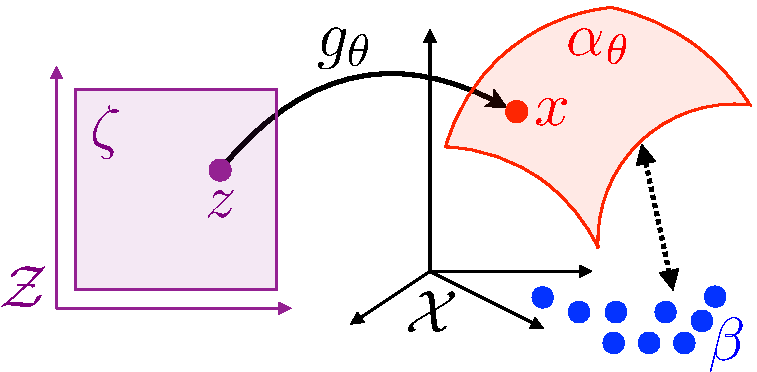
\includegraphics[width=.4\linewidth]{density-fitting/schematic-fitting}
\caption{\label{fig-density-fitting}
Schematic display of the density fitting problem~\ref{eq-density-fitting}.
}
\end{figure}


\newcommand{\fPF}{h}

This MLE approach is known to lead to optimal estimation procedures in many cases (see for instance~\cite{owen2001empirical}). However, it fails to work when estimating singular distributions, typically when the $\al_\th$ does not has a density (so that $\Ll_{\text{MLE}}(\al_\th,\be) = +\infty$) or when $(x_i)_i$ are samples from some singular $\bar\be$ (so that the $\al_\th$ should share the same support as $\be$ for $\KL(\al|\bar\be)$ to be finite, but this support is usually unknown). Another issue is that in several cases of practical interest, the density $\density{\th}$ is inaccessible (or too hard to compute).

A typical setup where both problems (singular and unknown densities) occur is for so-called generative models, where the parametric measure is written as a push-forward of a fixed reference measure $\zeta \in \Mm(\Zz)$
\eq{
	\al_\th = \fPF_{\th,\sharp} \zeta \qwhereq \fPF_\th : \Zz \rightarrow \Xx
}
where the push-forward operator is introduced in Definition~\ref{defn-pushfwd}. The space $\Zz$ is usually low-dimensional, so that the support of $\al_\th$ is localized along a low-dimensional ``manifold'' and the resulting density is highly singular (it does not have a density with respect to Lebesgue measure).
%
Furthermore, computing this density is usually intractable, while generating i.i.d. samples from $\al_\th$ is achieved by computing $x_i=\fPF_\th(z_i)$ where $(z_i)_i$ are i.i.d. samples from $\zeta$.

In order to cope with such difficult scenario, one has to use weak metrics in place of the MLE functional $\Ll_{\text{MLE}}$, which needs to be written in dual form as 
\eql{\label{eq-dual-loss}
	\Ll(\al,\be) \eqdef 
	\umax{(\f,\g) \in \Cc(\X)^2} 
	\enscond{ \int_{\X} \f(x) \d\al(x) + \int_{\X} \g(x) \d\be(x) }{ (\f,\g) \in \Potentials}.
}
Dual norms exposed in~\S\ref{sec-dual-norms} correspond to imposing $\Potentials = \enscond{(\f,-\f)}{\f \in B}$, while optimal transport~\eqref{eq-dual-generic} sets $\Potentials = \Potentials(c)$ as defined in~\eqref{eq-dfn-pot-dual}. 

For a fixed $\th$, evaluating the energy to be minimized in~\eqref{eq-density-fitting} using such a loss function corresponds to solving a semi-discrete optimal transport, which is the focus of Chapter~\ref{c-algo-semidiscr}. Minimizing the energy with respect to $\th$ is much more involved, and is typically highly non-convex.

The class of estimators obtained using $\Ll=\MK_\c$, often called ``Minimum Kantorovitch Estimators'' (MKE), was initially introduced in~\cite{bassetti2006minimum}, see also~\cite{CanasRosasco}.


%%%%%%%%%%%%%%%%%%%%%%%%%%%%%%%%%%%%%%%%%%%%%%%%%%%%%%%%%%%%%%%%%%%%%%%%%
\subsection{Wasserstein Derivatives}

\todo{Write me.}

Eulerian vs Lagrangian. 

Derivatives. 

Sinkhorn smoothing. 



%%%%%%%%%%%%%%%%%%%%%%%%%%%%%%%%%%%%%%%%%%%%%%%%%%%%%%%%%%%%%%%%%%%%%%%%%%%
\subsection{Sample Complexity}

In an applied setting, given two input measures $(\al,\be) \in \Mm_+^1(\X)^2$, an important statistical problem is to approximate the (usually unknown) divergence $D(\al,\be)$ using only samples $(x_i)_{i=1}^n$ from $\al$ and $(y_j)_{j=1}^m$ from $\be$. These samples are assumed to be independently identically distributed from their respective distributions. 
%
For both Wasserstein distances $\Wass_p$ (see~\ref{eq-defn-wass-dist}) and MMD norms (see \S\ref{sec-dual-norms}), a straightforward estimator of the unknown distance between distributions is compute it directly between the empirical measures, hoping ideally that one can control the rate of convergence of the latter to the former,
\eq{
	D(\al,\be) \approx D(\al_n,\be_m) \qwhereq
	\choice{
		\al_n \eqdef \frac{1}{n}\sum_i \de_{x_i},\\ 
		\be_m \eqdef \frac{1}{m}\sum_j \de_{y_j}.
	}
}
Note that here both $\al_n$ and $\be_m$ are random measures, so $D(\al_n,\be_m)$ is a random number. 
% 
For simplicity, we assume that $\X$ is compact (handling unbounded domain requires extra constraints on the moments of the input measures).

For such a dual distance that metrizes the weak convergence (see Definition~\ref{dfn-weak-conv}), since there is the weak convergence $\hat\al_n \rightarrow \al$, one has $D(\al_n,\be_n) \rightarrow D(\al,\be)$ as $n \rightarrow +\infty$.
%
But an important question is the speed of convergence of $D(\al_n,\be_n)$ toward $D(\al,\be)$, and this rate is often called the ``sample complexity'' of $D$. 

% Note that for $D(\al,\be) = \norm{\cdot}_{\TV}$, since the TV norm does not metrize the weak convergence, $\norm{\al_n - \be_n}_{\TV}$ is not a consistent estimator, namely it does not converge toward $\norm{\al-\be}_{\TV}$. Indeed, with probability 1, $\norm{\al_n - \be_n}_{\TV}=2$ since the support of the two discrete measures does not overlap. Similar issues arise with other $\phi$-divergences, which cannot be estimated using divergences between empirical distributions.

%%%%
\paragraph{Rates for OT.}

For $\X=\RR^\dim$ and measure supported on bounded domain, it is shown by~\cite{dudley1969speed} that for $\dim>2$, and $1 \leq p < +\infty$,  
\eq{
	\EE( |\Wass_p(\al_n,\be_n)-\Wass_p(\al,\be)| ) = O(n^{-\frac{1}{\dim}}),
}
where the expectation $\EE$ is taken with respect to the random samples $(x_i,y_i)_i$. This rate is tight in $\RR^\dim$ if one of the two measures has a density with respect to the Lebesgue measure. This result was proved for general metric spaces~\cite{dudley1969speed} using the notion of covering numbers and was later refined, in particular for $\X=\RR^d$ in~\cite{dereich2013constructive,fournier2015rate}. 
% Proof on $\Wass_1$ implies on $\Wass_p$ for $1 \leq p < +\infty$ by monotonicity in $p$.
This rate can be refined when the measures are supported on low-dimensional subdomains:~\cite{weed2017sharp} show that, indeed, the rate depends on the intrinsic dimensionality of the support. \cite{weed2017sharp} also study the nonasymptotic behavior of that convergence, such as for measures which are discretely approximated (\emph{e.g.} mixture of Gaussians with small variances).
%
It is also possible to prove concentration of $\Wass_p(\al_n,\be_n)$ around its mean $\Wass_p(\al,\be)$; see~\cite{bolley2007quantitative,boissard2011simple,weed2017sharp}.

%%%
\paragraph{Rates for MMD.}

For weak norms $\norm{\cdot}^2_{\Krkhs}$ which are dual of RKHS norms (also called MMD), as defined in~\eqref{eq-kernel-dual}, and contrary to Wasserstein distances, the sample complexity rate does not depend on the ambient dimension 
\eq{
	\EE( |\norm{\al_n-\be_n}_{\Krkhs}^2 - \norm{\al-\be}_{\Krkhs}^2 |^2 )
	= 
	O(n^{-\frac{1}{2}}), 
}
see~\cite{sriperumbudur2012empirical}. Note however that the constant appearing in this rate might depend on the dimension. 
%
This corresponds to the classical rate when using a Monte-Carlo method to estimate an integral using random samples. 
% 
For instance, one has, denoting $\xi=\al-\be$ and $\xi_n=\al_n-\be_n$
\eq{
	\EE( |\norm{\xi_n}_{\Krkhs} - \norm{\al-\be}_{\Krkhs} | ) 	= 
	\EE( |\int k \d(\xi \otimes \xi - \xi_n \otimes \xi_n)|^2 ).
}

\todo{Explain that this corresponds to the Monte-Carlo approximation of integrals using sums. Explain that the constant might depends on the dimension. Give a proof. }

%
% Figure~\ref{fig-sample-complexity} shows a numerical comparison of the sample complexity rates for Wasserstein and MMD distances.  
%
%Note, however, that $\norm{\al_n-\be_n}_{\Krkhs}^2$ is a slightly biased estimate of $\norm{\al-\be}_{\Krkhs}^2$. In order to define an unbiased estimator, and thus to be able to use, for instance, SGD when minimizing such losses, one should rather use the unbiased estimator 
%\begin{align*}
%	\text{MMD}_{\Krkhs}(\al_n,\be_n)^2 & \eqdef
%		\frac{1}{n(n-1)} \sum_{i,i'} \Krkhs(x_i,x_{i'})	+
%		\frac{1}{n(n-1)}\sum_{j,j'} \Krkhs(y_j,y_{j'}) \\
%		 & \qquad - 2
%		\frac{1}{n^2}\sum_{i,j} \Krkhs(x_i,y_j), 
%\end{align*}
%which should be compared to~\eqref{eq-mmd-discr}. It satisfies $\EE(\text{MMD}_{\Krkhs}(\al_n,\be_n)^2) = \norm{\al-\be}_{\Krkhs}^2$; see~\cite{gretton2012kernel}.



%%%
\paragraph{Rates for Sinkhorn.}

\todo{Give the intuition : smoothness of the potentials, Sobolev ball. }




\section{Gradient Flows}




%%%%%%%%%%%%%%%%%%%%%%%%%%%%%%%%%%%%%%%%%%%%%%%%%%%%%%%%%%%%%%%%%%%%%%%%%%%
\subsection{Optimization over Measures}

Example : neural net training, super-resolution, and other functional over measures.

Eulerian vs Lagrangian derivative 
   

%%%%%%%%%%%%%%%%%%%%%%%%%%%%%%%%%%%%%%%%%%%%%%%%%%%%%%%%%%%%%%%%%%%%%%%%%%%
\subsection{Particle System and Lagrangian Flows}

The intuition : at a Lagrangian OT as $\ell_2$ metric on points. OT flow is a flow on particle locations. 

Gradient descent schemes.

Study of mean field limits.

%%%%%%%%%%%%%%%%%%%%%%%%%%%%%%%%%%%%%%%%%%%%%%%%%%%%%%%%%%%%%%%%%%%%%%%%%%%
\subsection{Wasserstein Gradient Flows}

Implicit stepping. 

Fokker planck, 

Unbalanced gradient flows. 


%%%%%%%%%%%%%%%%%%%%%%%%%%%%%%%%%%%%%%%%%%%%%%%%%%%%%%%%%%%%%%%%%%%%%%%%%%%
\subsection{Langevin Flows}

1 random particles as opposed to many deterministic particles. Crucial in high dimension. 
% !TEX root = ../CourseOT.tex

%%%%%%%%%%%%%%%%%%%%%%%%%%%%%%%%%%%%%%%%%%%%%%%%%%%%%%%%%%%%%%%%%%%%%%%%%%%
%%%%%%%%%%%%%%%%%%%%%%%%%%%%%%%%%%%%%%%%%%%%%%%%%%%%%%%%%%%%%%%%%%%%%%%%%%%
%%%%%%%%%%%%%%%%%%%%%%%%%%%%%%%%%%%%%%%%%%%%%%%%%%%%%%%%%%%%%%%%%%%%%%%%%%%
\section{Extensions}

%%%%%%%%%%%%%%%%%%%%%%%%%%%%%%%%%%%%%%%%%%%%%%%%%%%%%%%%%%%%%%%%%%%%%%%%%%%
\subsection{Dynamical formulation}

%%%%%%%%%%%%%%%%%%%%%%%%%%%%%%%%%%%%%%%%%%%%%%%%%%%%%%%%%%%%%%%%%%%%%%%%%%%
\subsection{Unbalanced OT}

%%%%%%%%%%%%%%%%%%%%%%%%%%%%%%%%%%%%%%%%%%%%%%%%%%%%%%%%%%%%%%%%%%%%%%%%%%%
\subsection{Gromov Wasserstein}


Optimal transport needs a ground cost $\C$ to compare histograms $(\a,\b)$, it can thus not be used if the histograms are not defined on the same underlying space, or if one cannot pre-register these spaces to define a ground cost. 
%
To address this issue, one can instead only assume a weaker assumption, namely that one has at its disposal two matrices $\distD \in \RR^{n \times n}$ and $\distD' \in \RR^{m \times m}$ that represent some relationship between the points on which the histograms are defined. A typical scenario is when these matrices are (power of) distance matrices.
%
The Gromov-Wasserstein problem reads
\eql{\label{eq-gw-def}
	\GWD( (\a,\distD), (\b,\distD') )^2 \eqdef
	\umin{ \P \in \CouplingsD(\a,\b) } 
		\Ee_{\distD,\distD'}(\P) \eqdef 
		\sum_{i,j,i',j'} |\distD_{i,i'} - \distD'_{j,j'}|^2 \P_{i,j}\P_{i',j'}.  
}
This is a non-convex problem, which can be recast as a Quadratic Assignment Problem (QAP)~\cite{loiola-2007} and is in full generality NP-hard to solve for arbitrary inputs. 
%
It is in fact equivalent to a graph matching problem~\cite{lyzinski-2015} for a particular cost.

One can show that $\GWD$ satisfies the triangular inequality, and in fact it defines a distance between metric spaces equipped with a probability distribution (here assumed to be discrete in definition~\eqref{eq-gw-def}) up to isometries preserving the measures.
%
This distance was introduced and studied in details by Memoli in~\cite{memoli-2011}. An in-depth mathematical exposition (in particular, its geodesic structure and gradient flows) is given in~\cite{SturmGW}. See also~\cite{schmitzer2013modelling} for applications in computer vision.
%
This distance is also tightly connected with the Gromov-Hausdorff distance~\cite{gromov-2001} between metric spaces, which have been used for shape matching~\cite{memoli-2007,bronstein-2010}. 



%%%%%%%%%%%%%%%%%%%%%
\begin{rem}{Gromov-Wasserstein distance}
	The general setting corresponds to computing couplings between metric measure spaces $(\X,\dist_\X,\al_\X)$
	and $(\Y,\dist_\Y,\al_\Y)$ where $(\dist_\X,\dist_\Y)$ are distances and $(\al_\X,\al_\Y)$ are measures on their respective spaces.
	%
	One defines 
	\begin{align}
		\label{eq-gw-generic}
		\GW( (\al_\X,\dist_\X), (\al_\Y,\dist_\Y) )^2 \eqdef 
		\umin{ \pi \in \CouplingsD(\al_\X,\al_Y) } 
		\int_{\X^2 \times \Y^2}
		| \dist_\X(x,x')-\dist_\Y(y,y') |^2
		\d\pi(x,y)\d\pi(x',y').
	\end{align}
	$\GW$ defines a distance between metric measure spaces up to isometries, where one says that $(\al_\X,\dist_\X)$ and $(\al_\Y,\dist_\Y) $ are isometric if there exists $\phi : \X \rightarrow \Y$ such that $\phi_{\sharp}\al_\X=\al_\Y$ and $\dist_\Y(\phi(x),\phi(x'))=\dist_\X(x,x')$.
\end{rem}
%%%%%%%%%%%%%%%%%%%%%



%%%%%%%%%%%%%%%%%%%%%
\begin{rem}{Gromov-Wasserstein geodesics}
The space of metric spaces (up to isometries) endowed with this $\GW$ distance~\eqref{eq-gw-generic} has a geodesic structure. \cite{SturmGW} shows that the geodesic between  $(\X_0,\dist_{\X_0},\al_0)$ and $(\X_1,\dist_{\X_1},\al_1)$ can be chosen to be 
$t \in [0,1] \mapsto (\X_0 \times \X_1,\dist_t,\pi^\star)$ where $\pi^\star$ is a solution of~\eqref{eq-gw-generic} and for all $((x_0,x_1), (x_0',x_1')) \in (\X_0 \times \X_1)^2$, 
\eq{
	\dist_t((x_0,x_1), (x_0',x_1')) \eqdef
	(1-t)\dist_{\X_0}(x_0,x_0') + t\dist_{\X_1}(x_1,x_1').
}
This formula allows one to define and analyze gradient flows which minimize functionals involving metric spaces, see~\cite{SturmGW}. It is however difficult to handle numerically, because it involves computations over the product space $\X_0 \times \X_1$. 
%
A heuristic approach is used in~\cite{peyre2016gromov} to define geodesics and barycenters of metric measure spaces while imposing the cardinality of the involved spaces and making use of the entropic smoothing~\eqref{eq-gw-entropy} detailed below.
\end{rem}
%%%%%%%%%%%%%%%%%%%%%

To approximate the computation of $\GWD$, and to help convergence of minimization schemes to better minima, one can consider the entropic regularized variant
\eql{\label{eq-gw-entropy}
	\umin{ \P \in \CouplingsD(\a,\b) } 
		\Ee_{\distD,\distD'}(\P) - \epsilon \HD(\P).
}
As proposed initially in~\cite{gold-1996,rangarajan-1999}, and later revisited in~\cite{2016-solomon-gw} for applications in graphics, one can use iteratively Sinkhorn's algorithm to progressively compute a stationary point of~\eqref{eq-gw-entropy}. 
%
Indeed, successive linearizations of the objective function lead to consider the succession of updates
\eql{\label{eq-gw-sinkh}
	\itt{\P} \eqdef \umin{ \P \in \CouplingsD(\a,\b) } \dotp{\P}{\it{\C}} - \epsilon\H(\P)
		\qwhereq
}
\eq{
		\it{\C} \eqdef \nabla \Ee_{\distD,\distD'}(\it{\P}) = -\transp{\distD'} \it{\P} \distD, 
}
which can be interpreted as a mirror-descent scheme~\cite{2016-solomon-gw}. Each update can thus be solved using Sinkhorn iterations~\eqref{eq-sinkhorn} with cost $\it{\C}$. Figure~\eqref{fig-gw} illustrates the use of this entropic Gromov-Wasserstein to compute soft maps between domains. 


\begin{figure}
\centering
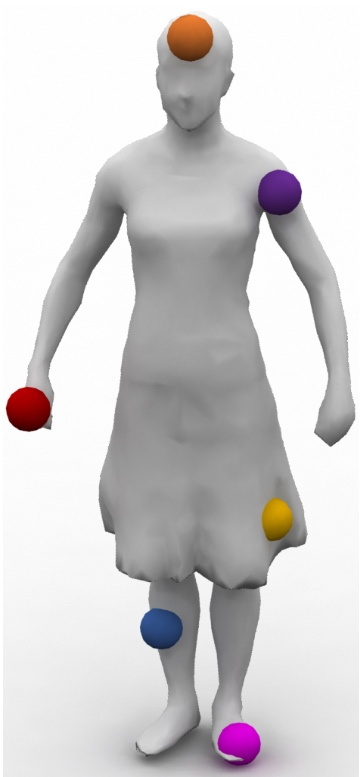
\includegraphics[height=.22\linewidth]{gw/source}
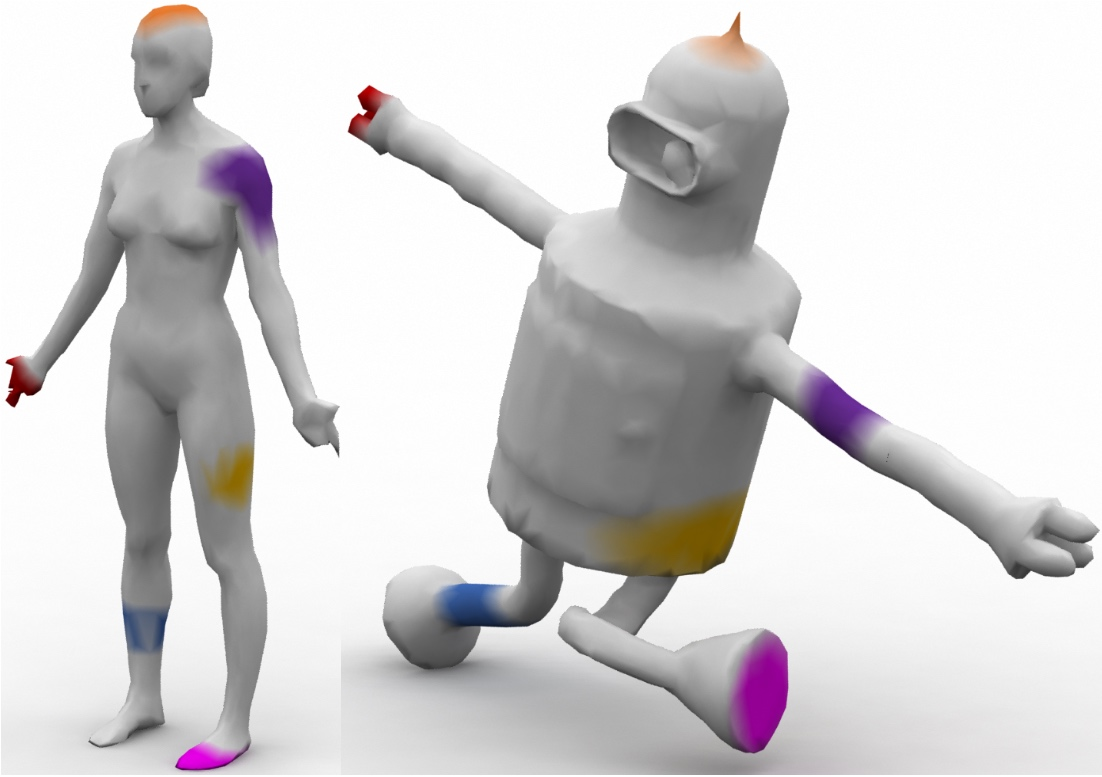
\includegraphics[height=.22\linewidth]{gw/target-surf}
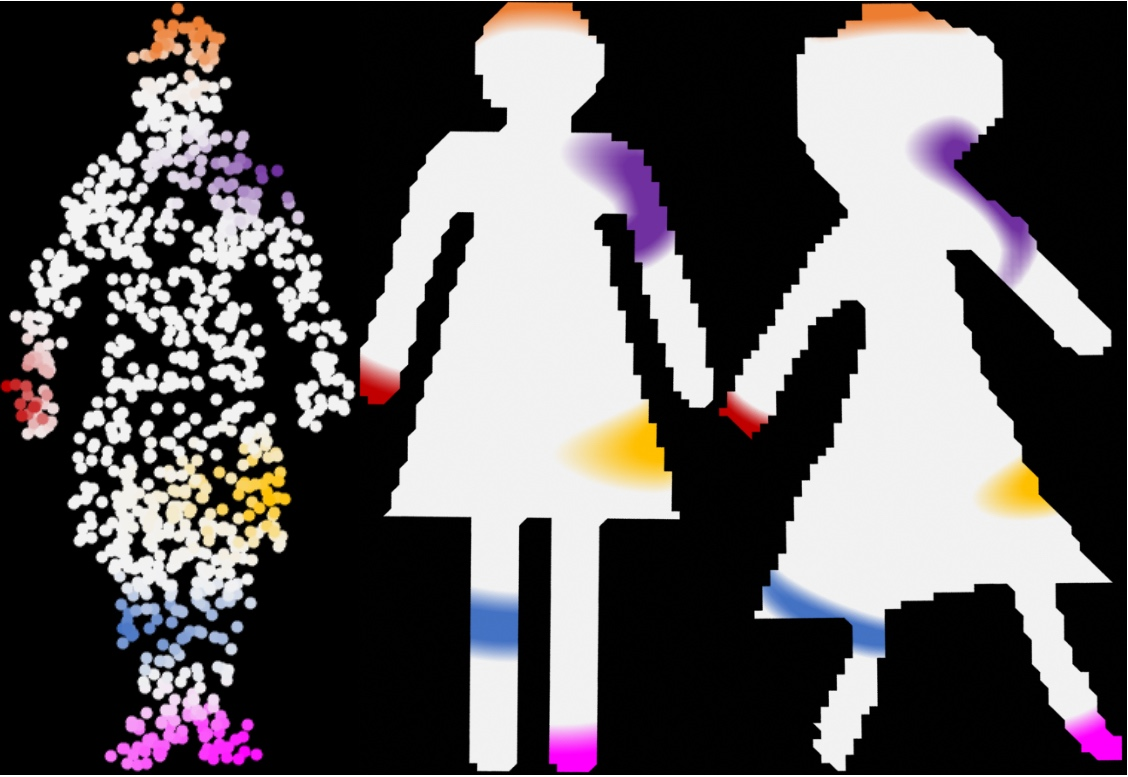
\includegraphics[height=.22\linewidth]{gw/target-2d}
\caption{\label{fig-gw}
Example of fuzzy correspondences computed by solving GW problem~\eqref{eq-gw-entropy} with Sinkhorn iterations~\eqref{eq-gw-sinkh}. Extracted from~\cite{2016-solomon-gw}.
}
\end{figure}


%%%%%%%%%%%%%%%%%%%%%%%%%%%%%%%%%%%%%%%%%%%%%%%%%%%%%%%%%%%%%%%%%%%%%%%%%%%
\subsection{Quantum OT}

Static formulation.

Gurvits algorithm, Q-sinkhorn.



% \nocite{*}

\bibliographystyle{plain}
\bibliography{all}

\end{document}
